\documentclass[pdftex,12pt,a4paper,oneside]{book}
\usepackage[australian]{babel}
\usepackage{graphicx,color}
\usepackage{epsf,verbatim}
\textheight = 257 true mm
\textwidth  = 160 true mm
\hoffset    = -12 true mm
\voffset    = -30 true mm

\usepackage[pdftex,colorlinks,plainpages=false]{hyperref}
%\usepackage[style=list,number=page]{glossary}
%\makeglossary

% \+ permits optional breaking of a word across lines without the 
% hyphen.
\newcommand{\+}{\discretionary{}{}{}}
\newcommand{\link}{\htmladdnormallink}

\begin{document}        % The beginning of the document.

%\bibliographystyle{amsplain}

\title{ESyS-Particle Tutorial and User's Guide \\ Version 2.3.1}
                                                                                
\author{D. Weatherley, W. Hancock \& V. Boros\\\small{The University of Queensland}
\\ S. Abe \\\small{Institute for Geothermal Resource Management}  
}
\date{\today}

\maketitle

\section*{Preface}
This document provides an introduction to Discrete Element Method (DEM) modelling using the ESyS-Particle Simulation Software developed by the \link{Centre for Geoscience Computing}{http://earth.uq.edu.au/centre-geoscience-computing} at \link{The University of Queensland}{http://www.uq.edu.au}. The guide is intended for new users and is written as a step-by-step tutorial on the basic principles and usage of the ESyS-Particle software. Readers are encouraged to obtain \link{a copy of the software}{https://launchpad.net/esys-particle/} and try the examples presented here. Readers are assumed to have had some experience using \link{Python}{http://www.python.org} and to be familiar with the fundamental principles of the DEM. If you have never used Python before, the \link{Python Language Tutorial}{http://docs.python.org/tut/tut.html} is an excellent starting point.


\tableofcontents

\listoffigures

%EXAMPLE FOR MAKING GLOSSARY ENTRIES
%NOAA\glossary{name=NOAA, 
%description=National Oceanographic and Atmospheric Administration,format=textbf}

%EXAMPLE FOR CITING PAPERS
%Impact of NTHMP on PTWC~\cite{McCreery2001}

\chapter[Introduction]{Introduction to the ESyS-Particle DEM simulation software}


The Discrete Element Method (DEM; Cundall and Strack~1979) is a popular numerical method for simulating the dynamics of brittle-elastic or granular materials. Materials are represented as assemblies of spherical particles, each of which may interact with neighbouring particles or other objects (such as planar walls) via simplified force-displacement interaction laws. The numerical solution involves computing the net force acting on each particle at a given time, then updating particle velocities and positions via an explicit finite difference integration scheme. Depending on the application of interest, many thousands (or even millions) of particles may be required and simulations may consist of up to millions of timesteps. The heavy computational burden of the DEM relative to other numerical methods is often the single most limiting factor determining the quality and utility of simulation results. 

ESyS-Particle is an Open Source implementation of the DEM designed for execution on multi-core Personal Computers (PCs), clusters or supercomputers running Linux-based operating systems. A modular, object-oriented DEM simulation engine written in C++ comprises the core of the software. Spatial domain decomposition is implemented using a master-slave strategy with inter-process communications using the Message Passing Interface (MPI) 1.0 standard. A verlet list neighbour search algorithm is implemented for detecting neighbouring particles and a variety of interaction laws are implemented for bonded or unbonded interactions between particles. Particles may have up to three translational and three rotational degrees of freedom as well as thermal properties. An explicit first-order finite difference time integration scheme is employed. Provision is made for file storage of both the entire model state or specific field variables during simulations.

Since the applications for the DEM are broad and varied, ESyS-Particle provides a simple Application Programming Interface (API) allowing users to design simulations via scripts written in the \link{Python}{http://www.python.org} programming language. For numerous applications, there is no need to modify the C++ simulation engine or re-compile the software. The Python API allows users to
\begin{itemize}
\item specify the initial locations and properties of particles and walls, 
\item define the types of interactions acting on these objects,
\item select the types and frequency of data output during simulations, and
\item perform user-defined computations at regular intervals via \texttt{Runnable} modules.
\end{itemize}

This User's Guide provides a tutorial-based introduction to DEM modelling using ESyS-Particle. The focus is on usage of the Python API to design and execute DEM simulations. In later chapters of the tutorial, instruction is provided on the use of post-processing tools packaged with ESyS-Particle, as well as third-party software or libraries for simulation construction and post-analysis. New users are encouraged to install ESyS-Particle on a PC and work through the following chapters consecutively. Additional features and tools are introduced gradually in the context of a number of common applications for the DEM, namely:
\begin{itemize}
\item ideal gas dynamics involving collisions between indivisible particles,
\item gravitational acceleration of individual particles or bonded groups of particles,
\item sandpiles and landslides,
\item hopper (or silo) flow, 
\item brittle failure of solids under uniaxial compression, and
\item shear of granular media within an annular shear cell apparatus.
\end{itemize}

\vskip 5mm
\begin{minipage}{5.75in}
\emph{\textbf{DISCLAIMER:} The simulation scripts described in this Guide and provided in the appendices are for instructional purposes only. These scripts are not considered production-ready for applied numerical modelling, and parameter values used may not lie in physical ranges for the application areas discussed. No warranty or guarantee is given by the authors as to the utility of these scripts for research and development purposes. It is the responsibility of the user to ensure ESyS-Particle simulations are verifiable and validated for any particular application.}
\end{minipage}
\vskip 5mm

\chapter{Simple Models}
\section{A simple simulation: collision of two particles}

This section introduces the basic features of ESyS-Particle simulation scripts via a simple example: collision of two indivisible particles. The simulation consists of two particles of differing mass whose initial velocities are selected to ensure that the particles will collide. This example serves to illustrate the main components of any ESyS-Particle simulation script, namely:

\begin{itemize}
   \item Initialisation of an ESyS-Particle simulation object
   \item Specification of the spatial domain
   \item Particle creation and initialisation
   \item Definition of inter-particle interactions
   \item Execution of time integration
\end{itemize}

The complete code-listing for this example is provided in Appendix~\ref{code:bingle}, entitled \texttt{bingle.py}\footnote{``Bingle'' is slang for a minor car crash or collision. Given our simulation setup, it seemed an appropriate name.}. It is recommended that you work through each section below, copying the code fragments as you go rather than simply copying the complete script. Code-fragments are identifiable by the \texttt{teletext font}. Shell commands will be prepended with the \$ symbol.

\subsection{Initialisation of an ESyS-Particle simulation}

In order to use the ESyS-Particle simulation libraries in Python, we must first import the modules we wish to use. For this first example, only the following two import statements are required:

\begin{verbatim}
from esys.lsm import *
from esys.lsm.util import Vec3, BoundingBox
\end{verbatim}

The first import statement loads a number of relevent classes and subroutines required for all ESyS-Particle simulations. The second statement imports the \texttt{Vec3} and \texttt{BoundingBox} classes. Objects of the \texttt{Vec3} class are 3-component vectors, useful for specifying position, velocity or acceleration vectors in 3D. \texttt{BoundingBox} objects specify a rectangular region of 3D space and typically denote the spatial extents of a domain or particle assembly.

Every ESyS-Particle simulation commences with the creation of an ESyS-Particle simulation object called \texttt{LsmMpi}. This object provides a means to define and run a simulation and can be thought of as a container to which we add simulation components such as a list of particles, walls, different types of interactions and data output components. The following code-fragment creates a simulation object:

\begin{verbatim} 
sim = LsmMpi(numWorkerProcesses=1, mpiDimList=[1,1,1])
sim.initNeighbourSearch(
   particleType="NRotSphere",
   gridSpacing=2.5,
   verletDist=0.5
)
\end{verbatim} 

The first statement creates an \texttt{LsmMpi} object and takes two arguments. The \texttt{numWorker\+Processes} argument specifies the number of MPI processes to use for calculations. In this example we choose to run a serial simulation (with only one worker process).  However we could just as easily set this argument to a larger value for a MPI-parallel simulation (if you have access to a computer with multiple processor cores/CPUs). The second argument (\texttt{mpiDimList}) specifies the manner in which the domain will be divided amongst the worker processes. The first coordinate refers to the number of subdivisions in the x-direction whilst the second and third coordinates specify the number of subdivisions in the y- and z-directions respectively. It is important that you set \texttt{numWorkerProcesses} to be equal to the total number of subdomains specified by the \texttt{mpiDimList}.

The second statement (\texttt{sim.initNeighbourSearch}) specifies the type of particles used in the simulation. The two most common particle types are \texttt{NRotSphere} and \texttt{RotSphere}. \texttt{sim.initNeighbourSearch} also sets two parameters for the contact detection algorithm. The \texttt{gridSpacing} parameter defines the size of cubic cells used to identify contacting particles. This parameter needs to be larger than the maximum particle diameter. The \texttt{verletDist} parameter determines the frequency with which the contact lists are updated. If any particle moves a distance greater than \texttt{verletDist} the lists are updated. Optimal values for these two parameters satify the inequality \texttt{gridSpacing} $>$ $2$ $\times$ \texttt{maxRadius} $+$ \texttt{verletDist}. Reducing the \texttt{verletDist} will result in more accurate force calculations (because new contacts will be detected earlier) but the lists will be updated more frequently, which is computationally expensive. In most 
cases, the \texttt{gridSpacing} should be set to approximately $2.5 \times$ the maximum particle radius and the \texttt{verletDist} should be approximately $0.2 \times$ the minimum particle radius.

These two statements result in the construction of a suitable ESyS-Particle simulation object called \texttt{sim}. The simulation object now becomes a container to which we can add particles, walls, and various types of interactions. Before we do that, we need to specify how many timesteps to compute during the simulation and the timestep increment (in seconds):

\begin{verbatim}
sim.setNumTimeSteps(10000)
sim.setTimeStepSize(0.001)
\end{verbatim}

These two statements are relatively self-explanatory. A total of $10000$ timesteps will be computed, with a time increment of $0.001$~sec between each timestep. It is usually a good idea to set the timestep increment before creating particles or interactions. In some cases, the timestep increment is needed internally to correctly initialise interactions. 

\subsection{Specification of the spatial domain}

Prior to addition of particles, the simulation object must be assigned a valid spatial domain. Any particles or walls residing outside this domain are eliminated from force calculations and time integration.  The following code-fragment specifies the spatial domain for a simulation:

\begin{verbatim}
sim.setSpatialDomain (
   BoundingBox(Vec3(-20,-20,-20), Vec3(20,20,20))
)
\end{verbatim}

\noindent
The spatial domain is defined by a rectangular \texttt{BoundingBox}. In this example the spatial domain is a cube with side length of $40.0$~metres, with the left, bottom, back corner at the position $(x,y,z) = (-20, -20, -20)$. 

\subsection{Particle creation and initialisation}

There are a number of ways to create and add assemblies of particles to a simulation object. We will encounter a few of the most common methods in subsequent tutorials. For this example, we will insert two particles individually. The following code-fragment creates a particle and initialises its linear velocity:

\begin{verbatim}
particle=NRotSphere(id=0, posn=Vec3(-5,5,-5), radius=1.0, mass=1.0)
particle.setLinearVelocity(Vec3(1.0,-1.0,1.0))
sim.createParticle(particle)
\end{verbatim}

The first statement creates a \texttt{NRotSphere} object called \texttt{particle} whose \texttt{id} will be set to $0$ with a \texttt{radius} of $1.0$ metre, a \texttt{mass} of $1.0$ kilogram, and initially centred on the point $(x,y,z) = (-5,5,-5)$. The second statement initialises the linear velocity of the particle to $(V_x,V_y,V_z) = (1.0,-1.0,1.0)$~metres/second. Finally the third statement adds the newly created particle to our simulation object.

\vskip 5mm
\noindent \textbf{\emph{EXERCISE:} Add a second particle to the simulation object with \texttt{id} of $1$, a \texttt{radius} of $1.5$~m and a \texttt{mass} of $2.0$~kg. Set the initial position of the particle to $(5,5,5)$ and its linear velocity as $(-1,-1,-1)$ (HINT: simply copy the code-fragment above and modify as necessary).}


\subsection{Definition of inter-particle interactions}

Having added two particles to our simulation object, we must now specify the type of interactions between the particles if they should come into contact (which they will due to the carefully selected initial positions and velocities above). There are a number of different types of particle-particle interactions that may be used. We will encounter most of the more common interaction types in this and subsequent tutorials. For this example we will choose the simplest type of interaction -- linear elastic repulsion between non-rotational spheres. The following code-fragment achieves this:

\begin{verbatim}
sim.createInteractionGroup(
   NRotElasticPrms(
      name = "elastic_repulsion",
      normalK = 10000.0,
      scaling = True
   )
)
\end{verbatim}

This statement creates a so-called \texttt{InteractionGroup} for our simulation object. The particular type of interaction group created depends upon the parameter set provided as an argument. In this case the \texttt{NRotElasticPrms} parameter set specifies purely elastic interactions between unbonded non-rotational spheres, with an elastic stiffness of $10000$~N/m.  When \texttt{scaling} is \texttt{True} (the default), the normal stiffness scales with particle size.  The \texttt{name} argument assigns the \texttt{InteractionGroup} a unique user-defined label which can be used to extract information about particle pairs undergoing this type of interaction. At this stage we will ignore the \texttt{name}, but we will return to this in a later tutorial.

Depending upon the parameter set provided as an argument to the \texttt{cre\+ateIn\+ter\+ac\+tionGroup} subroutine, different types of interactions may be specified including body forces (e.g. gravity), particle-wall interactions and various types of particle-particle interactions. Some of these different interaction types will also be encountered in subsequent tutorials.

\subsection{Execution of time integration}

We have now done everything necessary to set up the simulation. All that remains is to instruct Python to go ahead and do all the computations:

\begin{verbatim}
sim.run()
\end{verbatim}

\noindent
Although this statement might appear to be something of an anti-climax, it is the most important, instructing ESyS-Particle to commence the simulation and compute forces and update particle positions repeatedly until the specified number of timesteps are completed. Once this command is executed, the C++ simulation engine takes control and no subsequent Python commands will be executed until the simulation is completed. In the next tutorial, we will encounter three different ways to instruct ESyS-Particle to execute additional python commands during the simulation.

\subsection{Running an ESyS-Particle simulation from the commandline}

Using your favorite text editor copy all the code-fragments above into a text file and save it as \texttt{bingle.py}. Make sure you insert all the code-fragments in the order they appear here (and don't forget to add the second particle). Having saved the script, we can run the simulation using the following shell command:

\begin{verbatim}
$ mpirun -np 2 `which esysparticle` bingle.py
\end{verbatim}

Since ESyS-Particle is designed to run in parallel using MPI, we need this complicated commandline. If you have a multi-processor computer, you can increase the number of processes (\texttt{np}) to run the simulation in parallel. (You will also need to suitably modify the \texttt{numWorkerProcesses} and \texttt{mpiDimList} arguments in the script.) The number after \texttt{np} should always be equal to (\texttt{numWorkerProcesses} + 1). This is because ESyS-Particle uses a master-slave parallelisation strategy. \texttt{numWorkerProcesses} specifies the number of slaves to use but MPI must initialise one extra process to act as the master.

\subsection*{What's next?}

No doubt if you got this far you are somewhat disappointed that the simulation did not appear to do anything. I can assure you that (unless you got some weird error messages\footnote{If you did receive errors, carefully compare your script with the complete code-listing in Appendix~\ref{code:bingle} to identify any typographical mistakes. Also make sure you indent the code exactly as shown here because Python is particular about indentation.}) the simulation has correctly computed the trajectories of both particles for an interval of $10$~sec. During that time the particles collided then bounced off each other, changing the velocities and directions of each particle. Of course all this happened only in computer memory. We did not instruct the simulation to output any data to file or the screen.  The following tutorial will describe three different ways that data can be output during simulations. At the end of this tutorial, you will have written a re-usable module for creating snapshot images of the 
particles in motion and will know how to find out information about individual particles during a simulation.

\newpage
\section{Data output during simulations}

This tutorial extends the \texttt{bingle.py} simulation constructed in the previous tutorial. The primary aim here is to introduce three ways to output data during simulations. We will first examine the simplest way to output data -- printing particle positions to the screen. The second method involves output of data to a text file using a built-in feature called a CheckPointer. Although these techniques are often very useful for testing purposes or postprocessing of simulation data, they are certainly not as visually satisfying as producing glossy images or movies of the particles in motion. Finally we will examine how one of the ESyS-Particle visualisation modules can be used to generate images of the particle assembly. 

A secondary aim of this tutorial is to demonstrate three different approaches for including your own code in ESyS-Particle scripts. These approaches are:
\begin{itemize}
\item direct insertion in the time-integration loop,
\item writing and calling a user-defined subroutine, and 
\item use of a user-defined \texttt{Runnable} module.
\end{itemize}

\noindent
The use of \texttt{Runnable} modules is arguably the best method, even though it appears complicated at first. \texttt{Runnables} have the advantage that they can be very easily reused for other simulations with little or no modification. In this way a user can build a library of helpful utilities for analysis and visualisation of simulation data. We will explain how to prepare and import your own modules, as well as how to configure your shell environment so that Python can find your modules easily.

\subsection{Printing simulation data to screen}

This example modifies our original \texttt{bingle.py} script so that the positions of both particles can be output to screen every 100 timesteps. This represents one of the most basic of data output operations and allows us to do our first real analysis of the simulation results (e.g.\ by utilising external software to plot particle positions vs.\ time). The complete code-listing for this example is provided in Appendix~\ref{code:bingle_output}, called \texttt{bingle\_output.py}. 

Replace the last line (\texttt{sim.run()}) of \texttt{bingle.py} with the following code-fragment:

\begin{verbatim}
N_max = sim.getNumTimeSteps()
for n in range (N_max):
   sim.runTimeStep()

   if (n%100==0):
      particles = sim.getParticleList()
      p1 = particles[0].getPosn()
      p2 = particles[1].getPosn()
      print n,p1,p2

sim.exit()
\end{verbatim}

\noindent
This time, rather than simply computing all $10000$ timesteps with a single subroutine call (\texttt{sim.run()}), we explicitly implement the time integration loop (via the \texttt{for}-statement). The \texttt{sim.runTimeStep()} subroutine call instructs the simulation object to compute only one timestep of the simulation.  

After the timestep is completed, we check whether 100 timesteps have passed (via the \texttt{if}-statement). If so, we firstly obtain a \texttt{particles} list from the simulation object by calling \texttt{sim.getParticleList()}. \texttt{particles} is a Python list data structure where each member of the list is an ESyS-Particle \texttt{NRotSphere} object. \texttt{NRotSphere} objects have a number of subroutines that permit the user to obtain various information about individual particles (e.g.\ particle position, velocity, mass, radius, etc.). For more information about the available subroutines refer to the \link{\texttt{NRotSphere} class documentation}{http://esys.geocomp.uq.edu.au/esys-particle_python_doc/current/pythonapi/html/esys.lsm.LsmPy.NRotSphere-class.html}.

\vskip 5mm
\begin{minipage}{5.75in}
\emph{\textbf{WARNING:} Care should be taken when using \texttt{sim.getParticleList()} in a simulation containing a very large number of particles. For large simulations, the amount of memory required to store the list by the master process may be very large. It is usually best to avoid using \texttt{sim.getParticleList()} if possible. In the next tutorial we will encounter another method (the \texttt{CheckPointer}) to store information about particles that avoids using a large amount of memory. }
\end{minipage}
\vskip 5mm


Having obtained the \texttt{particles} list, we can extract the current positions of each particle via the \texttt{particles[\#].getPosn()} subroutine calls. These subroutine calls return a \texttt{Vec3} vector containing the x-, y- and z-coordinates of a particle's centre-of-mass. Finally we output the timestep number (\texttt{n}) and the positions of both particles to screen (via the usual Python \texttt{print} statement).

\begin{figure}
\resizebox{\textwidth}{!}{
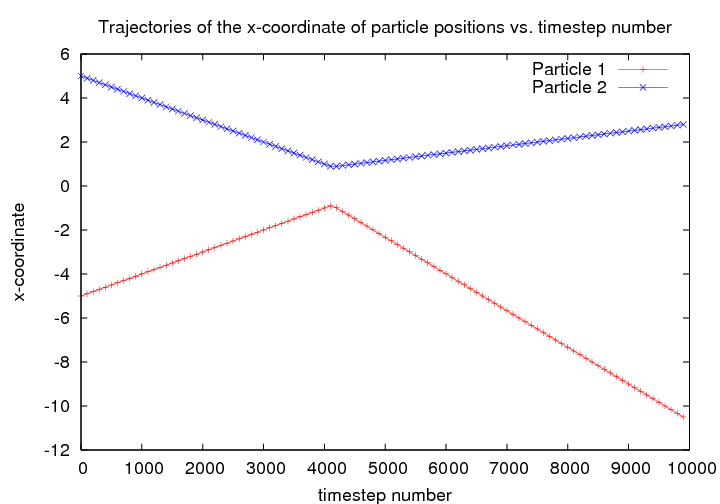
\includegraphics{bingle_output.jpg}}
\caption{A plot of particle trajectories using the text output (from \texttt{bingle\_output.py})} \label{fig:bingle_output}
\end{figure}

Save your modified script to a text file called \texttt{bingle\_output.py}, then run the simulation using the following shell command:

\begin{verbatim}
$ mpirun -np 2 `which esysparticle` bingle_output.py 
\end{verbatim}

\noindent
This shell command will run the simulation and output to screen the particle positions every 100 timesteps. An extract of 10 lines of output looks like:

\begin{verbatim}
1000 -3.999 3.999 -3.999 3.999 3.999 3.999
1100 -3.899 3.899 -3.899 3.899 3.899 3.899
1200 -3.799 3.799 -3.799 3.799 3.799 3.799
1300 -3.699 3.699 -3.699 3.699 3.699 3.699
1400 -3.599 3.599 -3.599 3.599 3.599 3.599
1500 -3.499 3.499 -3.499 3.499 3.499 3.499
1600 -3.399 3.399 -3.399 3.399 3.399 3.399
1700 -3.299 3.299 -3.299 3.299 3.299 3.299
1800 -3.199 3.199 -3.199 3.199 3.199 3.199
1900 -3.099 3.099 -3.099 3.099 3.099 3.099
\end{verbatim}

Re-run the simulation with the following shell command (typed on one line) to redirect the screen output to a text file called \texttt{simdata.csv}:

\begin{verbatim}
$ mpirun -np 2 `which esysparticle` bingle_output.py > simdata.csv
\end{verbatim}

\noindent
One can then use this text file to plot the trajectories of each particle, utilising your favourite graphing software. For example, import \texttt{simdata.csv} into a spreadsheet program and produce an XY plot of column two versus column one and column five versus column one. Your plot should be similar to Figure~\ref{fig:bingle_output}. Note that the two trajectories do not intersect although the particles are deflected in a manner consistent with collision. This is because the two particles are of finite radius and they collide only at their surfaces (whereas we are only plotting the trajectories of the centre-of-mass of the particles).

\subsection{Data output using the ESyS-Particle CheckPointer}

The simple example in the previous section is quite useful for debugging purposes, when one wishes only to monitor the movement of a few particles. In simulations involving many thousands of particles, one would prefer to output the positions, velocities and accelerations of all the particles at regular intervals so the data may be post-processed in various ways. ESyS-Particle includes a module known as a CheckPointer for this purpose. The CheckPointer is a special case of a group of modules known as FieldSavers, which we will discuss in a future tutorial. FieldSavers provide a mechanism to selectively output information on particles (such as position or kinetic energy), interactions (e.g.\ potential energy) and walls (including their position and the net force acting on a wall). 

A CheckPointer is designed to write text files at regular intervals containing the positions, velocities and accelerations of all particles. To implement a CheckPointer in a simulation is a relatively simple procedure. Return to your \texttt{bingle.py} script created in the first tutorial. Just before the \texttt{sim.run()} subroutine call, add the following code fragment:

\begin{verbatim}
sim.createCheckPointer (
   CheckPointPrms (
      fileNamePrefix = "bingle_data",
      beginTimeStep = 0,
      endTimeStep = 10000,
      timeStepIncr = 100
   )
)
\end{verbatim}

\noindent
The CheckPointer takes four parameters: 
\begin{itemize}
\item \texttt{fileNamePrefix}: specifying the filename prefix for all the output files to be written during the simulation,
\item \texttt{beginTimeStep}: the timestep number to commence saving data,
\item \texttt{endTimeStep}: the timestep number to conclude saving data, and
\item \texttt{timeStepIncr}: the number of timesteps to complete between each save.
\end{itemize}

\noindent
The example above will save simulation data every 100 timesteps, commencing at the first timestep (timestep \texttt{0}) and concluding at the last timestep (timestep \texttt{10000}). Often it is advantageous to save data for only a portion of the simulation at more regular intervals, particularly in cases where the interesting part of the simulation commences after a period of time (e.g.\ after the particles have settled under gravity). 

Append the code fragment above to \texttt{bingle.py} and save the script as \texttt{bingle\_chk.py}. Execute the simulation using the following command:

\begin{verbatim}
$ mpirun -np 2 `which esysparticle` bingle_chk.py
\end{verbatim}

Upon completion of the simulation, type \texttt{ls} at the command prompt. Failing any errors, you should have a listing similar to the following:

\begin{verbatim}
bingle_chk.py
bingle_data_t=0_0.txt
bingle_data_t=0_1.txt
bingle_data_t=10000_0.txt
bingle_data_t=10000_1.txt
bingle_data_t=1000_0.txt
bingle_data_t=1000_1.txt
bingle_data_t=100_0.txt
bingle_data_t=100_1.txt
bingle_data_t=1100_0.txt
bingle_data_t=1100_1.txt
bingle_data_t=1200_0.txt
bingle_data_t=1200_1.txt
...
\end{verbatim}

\noindent
You should notice there are two files generated at each designated save time: \texttt{bin\+gle\_\+da\+ta\_\+t=N\_0.txt} and \texttt{bingle\_data\_t=N\_1.txt}, where \texttt{N} denotes the timestep number when the file was saved. The first (ending with \texttt{\_0.txt}) is a header file containing information about the format of the corresponding data file (ending with \texttt{\_1.txt}). Depending upon the type of particles used, whether or not you have mesh walls etc., the format of the checkpoint files changes so that all relevant information about the simulation is saved at the specified times. 

Let's examine one of the output files from our simulation. Type \texttt{cat bin\+gle\_\+da\+ta\_\+t=0\_1.txt} at the command prompt. The result should look like this:

\begin{verbatim}
2
-5 5 -5 1 0 -1 1 -5 5 -5 -5 5 -5 1 -1 1 0 0 0 0 0 0
5 5 5 1.5 0 -1 2 5 5 5 5 5 5 -1 -1 -1 0 0 0 0 0 0
0
TMIG 0
\end{verbatim}

\noindent
The first line of the file specifies the number of particles in the simulation (only 2 in our case). The following 2 lines provide data on each of the particles, with one line per particle. We will examine the meaning of each number on these lines in a moment. After listing the data for each particle, the next line specifies the number of triangle mesh walls and the last line specifies the number of triangle mesh wall interaction groups. In our example we have no mesh walls or mesh wall interaction groups, hence the \texttt{0} on each line. We will revisit mesh walls in a later tutorial on hopper flow simulation.

Returning to the lines providing data on each particle, for simulations using \texttt{NRot\+Sphere} particles (as we are using here), the fields in each data line correspond to the following:
\begin{itemize}
\item fields 1, 2 \& 3: the X, Y and Z-coordinates of the \emph{current} particle position
\item field 4: the particle radius
\item field 5: the particle ID
\item field 6: the particle tag (more on tags later)
\item field 7: the particle mass (recall that we set the mass of the second particle to be \texttt{2.0})
\item fields 8, 9 \& 10: the X, Y and Z-coordinates of the \emph{initial} particle position
\item fields 11, 12 \& 13: the X, Y and Z-coordinates of the \emph{previous} particle position
\item fields 14, 15 \& 16: the X, Y and Z-components of the particle velocity
\item fields 17, 18 \& 19: the X, Y and Z-components of the net force acting on the particle
\item fields 20, 21 \& 22: (used with circular or periodic boundaries) specifies the circular shift to be added in the X, Y and Z-directions 
\end{itemize}

Your first impression may be that this is a lot of information to output for each particle when you may only be interested in, say, the velocities of each particle. The CheckPointer is designed to be a multi-purpose data output mechanism which records every piece of information on the current state of particles in the simulation. It is an ideal mechanism for outputing data when you intend to perform a number of different post-processing operations on your simulation data. The downside is that the CheckPointer can use a lot of disk space. To circumvent this problem, FieldSavers provide a mechanism to selectively output only certain data to disk. One needs to exercise caution when using FieldSavers because if you forget to store important information, you need to re-run the entire simulation. We will examine how to set up FieldSavers in a later tutorial on uniaxial compression of elastic-brittle material.

\subsection{Generation of particle snapshots (via subroutine calls)}

The previous two examples illustrated simple ways to output data from ESyS-Particle simulations. In this example we will introduce a way to generate beautiful snapshots of the particle assembly at various times during a simulation. This is achieved using the ESyS-Particle \texttt{esys.lsm.vis.povray} module and an external package called \link{POVray}{http://www.povray.org} that is ideal for generating images of 3D objects or scenes\footnote{Take a break for the moment and enjoy the amazing computer-generated images in the \link{POVray Hall of Fame}{http://hof.povray.org/}!}. The ESyS-Particle \texttt{povray} module provides a relatively simple interface between particle simulations and POVray. 

This part of the tutorial involves implementation of a Python subroutine. If you are not already familiar with writing subroutines in Python, I recommend you first study \link{Chapter 4 of the Python Language Tutorial}{http://docs.python.org/tut/node6.html}.  We will modify \texttt{bingle\_output.py} for this example.  The complete code-listing is available in Appendix~\ref{code:bingle_vis} entitled \texttt{bingle\_vis.py}.

Since we will be making use of the ESyS-Particle \texttt{povray} module, we need to add a third import statement to the top of our script: 

\begin{verbatim}
from esys.lsm.vis import povray
\end{verbatim}

\noindent
ESyS-Particle currently has two visualisation modules -- \texttt{povray} and \texttt{vtk}. Both utilise external libraries for rendering images of simulation data (\link{POVray}{http://www.povray.org} and \link{VTK}{http://www.vtk.org} respectively). The ESyS-Particle visualisation modules are designed to provide a common interface to these two rendering engines (so that either package may be used with minimal changes to your Python script). Each module has both advantages and disadvantages. \texttt{povray} produces very beautiful images of particle assemblies with the possibility of rendering particles with various textures and special effects, but it lacks tools specifically designed for scientific visualisation of datasets (e.g.\ for generating isosurfaces or contours). \texttt{vtk} is the opposite, providing great scientific visualisation tools and an interactive graphical interface but lacking strong support for rendering particles nicely. 

Having imported the \texttt{povray} module, we now implement a Python subroutine called \texttt{snapshot()} designed to render an image of the particle assembly and store it as a file. The code-fragment for implementing this subroutine is as follows:

\begin{verbatim}
def snapshot(particles=None, index=0):
   pkg = povray

   scene = pkg.Scene()

   for pp in particles:
      povsphere = pkg.Sphere(pp.getPosn(), pp.getRadius())
      povsphere.apply(pkg.Colors.Red)
      scene.add(povsphere)

   camera = scene.getCamera()
   camera.setLookAt(Vec3(0,0,0))
   camera.setPosn(Vec3(0,0,20))
   camera.setZoom(0.1)

   scene.render(
      offScreen=True, 
      interactive=False, 
      fileName="snap_%.4d.png" % (index), 
      size=[800,600]
   )
   return
\end{verbatim}

\noindent
The first line of this code-fragment defines the name of the subroutine (\texttt{snapshot}) and specifies that it accept two keyword arguments: 
\begin{itemize}
\item \texttt{particles} -- a pointer to a list of particles (e.g.\ obtained from the \texttt{sim.getPar\+tic\+leList()} subroutine), and
\item \texttt{index} -- a unique identifier used to specify the name of the file in which to store the rendered image. 
\end{itemize}

Within the subroutine, we firstly specify that the visualisation package (\texttt{pkg}) will be \texttt{povray}. We could just as easily have replaced \texttt{povray} with \texttt{vtk} to use the other renderer. Having selected the package, we then construct a \texttt{Scene} object via the \texttt{scene = pkg.Scene()} subroutine call. \texttt{Scene} objects are containers for \emph{actors}, a \emph{camera} and (optionally) a \emph{light-source}. \emph{Actors} can be any three-dimensional object we wish to see in the Scene. When defining actors, we specify the geometrical shape of the actor, its colour or surface texture, and its position and orientation in the Scene. 

ESyS-Particle visualisation modules provide support for a number of different primitive shapes that we can use as actors in our scene (e.g.\ spheres, cones, cylinders and boxes). In this tutorial we will stick with simple spheres to represent the particles in our simulation. To specify how our scene will look, we need to add spheres to the scene via the code-fragment:

\begin{verbatim}
   for pp in particles:
      povsphere = pkg.Sphere(pp.getPosn(), pp.getRadius())
      povsphere.apply(pkg.Colors.Red)
      scene.add(povsphere)
\end{verbatim}

\noindent
This code-fragment loops over each particle in the list provided by the \texttt{particles} argument. For each particle in the list, we create a sphere via the \texttt{pkg.Sphere(..)} subroutine, specify the colour of the sphere using \texttt{Sphere.apply(..)} then add the sphere to the scene using \texttt{scene.add(..)}. The \texttt{pkg.Sphere(..)} subroutine takes two mandatory arguments -- the position of the sphere (as a \texttt{Vec3} vector) and the radius of the sphere. In most cases we can simply use the original coordinate system and sizes of particles from our simulation. 

Next we must initialise the camera we will use to take a picture of our scene. This is an important step: if we do not initialise the camera correctly our rendered image may be empty or we may only see a portion of the scene. Typically you will need to experiment with the camera settings to achieve the desired result. In this case I have selected reasonable values for visualising our \texttt{bingle.py} simulation. The appropriate camera setup code-fragment is:

\begin{verbatim}
   camera = scene.getCamera()
   camera.setLookAt(Vec3(0,0,0))
   camera.setPosn(Vec3(0,0,20))
   camera.setZoom(0.1)
\end{verbatim}

\noindent
The first statement returns a pointer to our scene's camera which we call \texttt{camera}. Next we specify the point in 3D space we would like to be the focus of the camera (via the \texttt{camera.setLookAt(..)} subroutine). We also specify the position of the camera itself (\texttt{camera.setPosn(..)}) and finally we choose the zoom factor (\texttt{camera.setZoom(..)}). Changing the zoom factor is a good starting point if your rendered image is empty or doesn't look the way you desire.

Finally, we can instruct the \texttt{Scene} object to create an image of the scene we have just constructed:

\begin{verbatim}
   scene.render(
      offScreen=True,
      interactive=False,
      fileName="snap_%.4d.png" % (index),
      size=[800,600]
   )
\end{verbatim}

\noindent
This subroutine call instructs ESyS-Particle to communicate with the renderer library (either via a temporary script or directly via a socket interface) to generate an image of the scene. A number of optional keyword arguments may be provided to control various aspects of the final image:
\begin{itemize}
\item \texttt{offScreen} -- a Boolean variable that determines whether the image will appear in a window onscreen or be rendered offscreen (in the background). 
\item \texttt{interactive} -- a Boolean variable specifying whether the user is permitted to interact with the rendered image. If this argument is set to \texttt{True} and \texttt{offScreen=False}, a window will appear and the user will be able to pan and zoom the image using the mouse or keyboard. Only the \texttt{vtk} package provides interactive features.
\item \texttt{filename} -- a text string specifying the name of the file in which to save the image. The filename extension determines the image format. Both \texttt{povray} and \texttt{vtk} support a large range of common image formats. 
\item \texttt{size} -- a tuple specifying the pixel resolution of the final image. Changing the aspect ratio of this tuple can help you render the extremities of a particle assembly that is not 4:3 aspect ratio.
\end{itemize}

\noindent
Notice that the filename argument above uses Python string formatting syntax to construct a filename of the form \texttt{snap\_000\#.png} where \texttt{\#} is the index provided as the second argument of our \texttt{snapshot} subroutine. This naming convention is very handy for producing a sequence of images that can later be combined into a movie of the simulation.

In a copy of \texttt{bingle\_output.py} append the import statement and subroutine definition above directly after the two existing import statements. Having done this, all that remains is to replace the \texttt{if}-statement in the time integration loop with the following:

\begin{verbatim}
   if (n%100==0):
      particles = sim.getParticleList()
      snapshot(particles=particles, index=n)
\end{verbatim}

\noindent
Notice that we no longer \texttt{print} the particle positions to screen. Instead we call our new \texttt{snapshot()} subroutine providing, as arguments, the current list of particles returned by \texttt{sim.getParticleList()} and the current timestep number (\texttt{n}) as the index for naming the image file rendered when the subroutine is called.

Save the resulting script to a text file called \texttt{bingle\_vis.py} and run the simulation from the shell using a similar command as before. All being well, your simulation should now produce a sequence of 100 image files named \texttt{snap\_0000.png} through to \texttt{snap\_9900.png}. Figure~\ref{fig:bingle_vis} contains a few of these snapshots from various times during the simulation. The approach, collision and rebound of the particles is now clearly evident.

\begin{figure}
\begin{center}
\resizebox{5in}{!}{
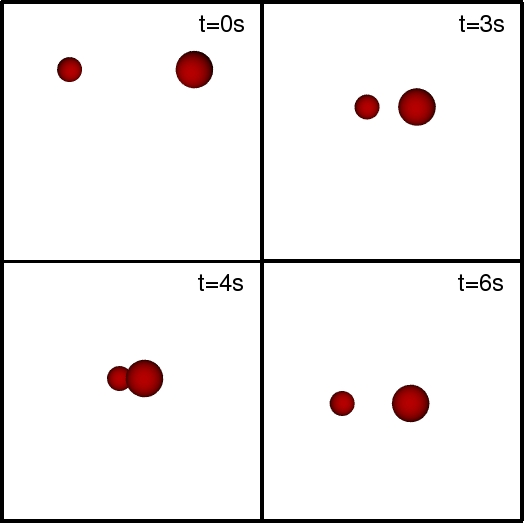
\includegraphics{bingle_vis_snaps_2.jpg}}
\end{center}
\caption{A sequence of snapshots (from \texttt{bingle\_vis.py})} \label{fig:bingle_vis}
\end{figure}

This tutorial example illustrates only very basic visualisation. However the \texttt{povray} package can be used to produce much more attractive images by using some of its more advanced features. In the next example we will describe how to write your own module for producing image snapshots that you can reuse for subsequent simulations with relatively minor additions to your simulation script.

\subsection{A \texttt{Runnable} module for generating snapshots}

Thus far in our data output examples we have had to make use of an explicit time-integration loop (instead of the simple and elegant \texttt{sim.run()} call), used a \texttt{CheckPointer} to store particle data and, in the previous example, have added an additional subroutine to our simulation script. This has resulted in a rather lengthy script. To compound the issue, we would need to do this for every simulation script we write, resulting in many large scripts containing much duplicate code. From a design and implementation perspective this is unwieldy and multiplies the possibility for errors in the code. 

ESyS-Particle provides a mechanism to resolve many of these issues in the form of a \texttt{Runnable} class. A \texttt{Runnable} is a user-defined class that can be called by a simulation object once per timestep either before or after the force computations and time-integration. \texttt{Runnable} classes can be implemented as modules that can be reused in subsequent simulations simply by adding an import statement and some lines of initialisation code to your simulation script. This is a powerful feature of ESyS-Particle, offering the user the possibility to develop runtime data analysis and visualisation utilities that can be reused whenever they are needed with little or no modification to the \texttt{Runnable} itself.  

The aim for this tutorial example is to implement the \texttt{snapshot()} subroutine from the previous example as a \texttt{Runnable} module. We will discuss how to call this from within your simulation script and how to deploy the module so that it can be easily reused in subsequent simulation scripts. If you are not already familiar with classes and inheritance in Python, I recommend you first study \link{Chapter 9 of the Python Language Tutorial}{http://docs.python.org/tut/node11.html}. We will also touch on some topics covered in \link{Chapter 6 of the Python Tutorial}{http://docs.python.org/tut/node8.html}. The complete code-listings for this example are found in Appendix~\ref{code:POVsnaps} \texttt{POVsnaps.py} and Appendix~\ref{code:bingle_Runnable} \texttt{bingle\_Runnable.py}.

\subsubsection{Implementation of a snapshot \texttt{Runnable}}

A \texttt{Runnable} is best implemented in its own text file rather than inserting it in a simulation script (although you may do this if you wish). We will implement our \texttt{Runnable} in a text file called \texttt{POVsnaps.py}. Like any other ESyS-Particle script, we commence with relevent import statements:

\begin{verbatim}
from esys.lsm import *
from esys.lsm.util import Vec3, BoundingBox
from esys.lsm.vis import povray
\end{verbatim}

A user-defined \texttt{Runnable} is a class that inherits from an ESyS-Particle base class called \texttt{Runnable}. As per any Python class, we must implement an initialisation subroutine (\texttt{self.\_\_init\_\_()}) that is called whenever we construct an instance of this class. The initialisation subroutine prepares an instance of the class for use in a simulation. The following code-fragment implements the class definition and initialisation subroutine:


\begin{verbatim}
class POVsnaps (Runnable):
   def __init__(self, sim, interval):
      Runnable.__init__(self)
      self.sim = sim
      self.interval = interval
      self.count = 0
      self.configure()
\end{verbatim}


The first line defines the name of the class \texttt{POVsnaps} and specifies that it inherits from the \texttt{Runnable} base class. Next we encounter the definition of the \texttt{\_\_init\_\_(..)} subroutine. Note that we have stipulated that this subroutine accepts two mandatory arguments: a pointer to the simulation object to which the class is attached (\texttt{sim}) and an integer (\texttt{interval}) specifying the number of timesteps between successive images. The \texttt{\_\_init\_\_(..)} subroutine first calls the equivalent base class subroutine to do some default initialisation of our \texttt{Runnable}, then stores the \texttt{sim} pointer and \texttt{interval} as data members of the class, as well as initialising a counter (\texttt{self.count}) that keeps track of the total number of images rendered. (We use this later to define the image filenames.) A \texttt{self.configure()} subroutine is also called, the implementation of which is as follows: 

\begin{verbatim}
   def configure(
      self, 
      lookAt=Vec3(0,0,0), 
      camPosn=Vec3(0,0,20), 
      zoomFactor=0.1,
      imageSize=[800,600]
   ):
      self.lookAt=lookAt
      self.camPosn=camPosn
      self.zoomFactor=zoomFactor
      self.imageSize=imageSize
\end{verbatim}

Our \texttt{self.configure()} subroutine accepts four optional keyword arguments: \texttt{lookAt}, \texttt{camPosn}, \texttt{zoomFactor} and \texttt{imageSize}. Each of these arguments is provided with a default value in the subroutine definition (the first line). When this subroutine is called, any keyword argument that is not assigned a value by the calling statement will be set to the default value specified here. The call to \texttt{self.configure()} in the initialisation subroutine specifies no keyword arguments, so all of these arguments will be set to their default values. The implementation of this subroutine is straight-forward: we simply create an internal data member to store the value for each argument. These data members will be used in the \texttt{self.snapshot()} subroutine later. 

\vskip 5mm
\begin{minipage}{5.75in}
\emph{\textbf{ASIDE:} You may be wondering why we have implemented an extra subroutine for configuring these data members. We could have included these as keyword arguments of the initialisation subroutine. The rationale for implementing this extra subroutine is that we can use this subroutine to reconfigure our \texttt{POVsnaps Runnable} during a simulation. This feature might be used, for example, to change the camera position during a simulation to produce a fly-through animation of the particle assembly. The initialisation subroutine can only be called once but the \texttt{configure(..)} subroutine can be called many times.}
\end{minipage}
\vskip 5mm

ESyS-Particle \texttt{Runnable} subclasses must also implement a \texttt{self.run()} subroutine. This subroutine is called by simulation objects once per timestep and it is here that we implement the code that should be executed by the \texttt{Runnable} each timestep. The following code-fragment implements the mandatory \texttt{self.run()} subroutine:

\begin{verbatim}
   def run(self):
      if ((self.sim.getTimeStep() % self.interval) == 0):
         self.snapshot()
         self.count += 1
\end{verbatim}

The \texttt{self.run()} subroutine simply waits until \texttt{self.interval} timesteps have elapsed, then calls the \texttt{self.snapshot()} subroutine prior to incrementing the counter. This code-fragment is reminiscent of the code we added to the time-integration loop of \texttt{bin\+gle\_\+vis.py}. Not surprisingly, the \texttt{self.snapshot()} subroutine looks very similar to the subroutine we encountered in that example: 

\begin{verbatim}
   def snapshot(self):
      pkg = povray
      Scene = pkg.Scene()
      plist = self.sim.getParticleList()

      for pp in plist:
         povsphere = pkg.Sphere(pp.getPosn(), pp.getRadius())
         povsphere.apply(pkg.Colors.Red)
         Scene.add(povsphere)

      camera = Scene.getCamera()
      camera.setLookAt(self.lookAt)
      camera.setPosn(self.camPosn)
      camera.setZoom(self.zoomFactor)

      fname = "snap_%.4d.png" % (self.count)
      Scene.render(
         offScreen=True, 
         interactive=False, 
         fileName=fname, 
         size=self.imageSize
      )
\end{verbatim}

\noindent
You will notice only a few minor differences though. We now use the data members defined in the \texttt{self.configure()} subroutine to initialise the camera and the image size. By using these data members we can easily configure our snapshot \texttt{Runnable} for different simulations or perhaps reconfigure the camera during a simulation if we would like, for example, to create a fly-through animation.

\subsubsection{Use of the snapshot \texttt{Runnable} in a simulation}

Having copied all the code-fragments into a text file called \texttt{POVsnaps.py}, we are ready to use our \texttt{Runnable} in a simulation. We will modify \texttt{bingle.py}, the script we wrote that didn't produce any data output. Firstly, add an import statement to the top of the script:

\begin{verbatim} 
from POVsnaps import POVsnaps
\end{verbatim} 

\noindent
This statement will instruct Python to search for a file called \texttt{POVsnaps.py} and import the \texttt{POVsnaps} class implemented therein. Having done this, Python now knows where to find the implementation of this class when we wish to use it. 

Now scroll down your simulation script and insert the following code-fragment just before the \texttt{sim.run()} statement:

\begin{verbatim}
povcam = POVsnaps(sim=sim, interval=100)
sim.addPostTimeStepRunnable(povcam)
\end{verbatim}

\noindent
The first statement creates a POVsnaps object called \texttt{povcam}. We have specified that it will be attached to our simulation object (\texttt{sim}) and snapshots will be taken every 100 timesteps. The second statement is all-important. This statement instructs the simulation object to add our \texttt{Runnable} as a ``\texttt{PostTimeStepRunnable}''. In other words, the \texttt{povcam.run()} subroutine will be called each timestep after the simulation object has completed force calculations and updated particle positions and velocities. We also have the possibility of adding a \texttt{Runnable} whose \texttt{run()} subroutine is called before force calculations. This is a ``\texttt{PreTimeStepRunnable}''.

Save your simulation script in a text file called \texttt{bingle\_Runnable.py} and run the simulation from the shell. The simulation will output snapshots of the particle assembly in much the same way as the \texttt{bingle\_vis.py} script in the previous example. Note that this time we only needed to add 3 statements to our simulation script to utilise the \texttt{Runnable} (as compared with \texttt{bingle\_vis.py} where we had to add approximately 19 lines of code, including the subroutine definition). We have not only avoided tiring out our fingers typing all those lines of code; we have created a module that can be reused in other simulation scripts just by adding the 3 lines of code above. 

\subsubsection{Deploying a \texttt{Runnable} as a reusable module}

Whenever Python encounters an import statement, it will search a number of default directories for the appropriate python scripts implementing the imported modules. These default directories are typically places like \texttt{/usr/lib/Python2.4/site-packages} or \linebreak \texttt{/usr/local/lib/Python2.4/site-packages}. If Python cannot find the script, it will search the current working directory. If Python still cannot find the script, it will crash with an error message. 

As a user, you have two options for reusing your \texttt{Runnable} module. Firstly you could copy your \texttt{Runnable} module script (e.g.\ \texttt{POVsnaps.py}) into the current working directory whenever you wish you use it. This can get tedious, so a better way is to copy the script to a directory where you intend to store all your useful \texttt{Runnable} module scripts. To do this first create a directory to store the scripts and copy your script into that directory:

\begin{verbatim}
$ mkdir /home/my_username/Runnable_scripts/
$ cp POVsnaps.py /home/my_username/Runnable_scripts
\end{verbatim}

\noindent 
(Don't forget to replace the word ``\texttt{my\_username}'' with you actual username!) Having done that you must add this directory to an environment variable called \texttt{PYTHONPATH}. In the bash shell, it is done this way:

\begin{verbatim}
$ export PYTHONPATH=/home/my_username/Runnable_scripts/:$PYTHONPATH
\end{verbatim}

\noindent
If you use a different shell, consult your shell documentation or ask your local linux guru or system administrator for help. You may wish to add the shell command above to a file that is executed whenever you open a shell (e.g.\ \texttt{/home/my\_username/.bashrc}).

Once your \texttt{Runnable\_scripts} directory is in your \texttt{PYTHONPATH}, Python will be able to find your module whenever it encounters an import statement like \texttt{from POVsnaps import POVsnaps}. You have now successfully deployed your \texttt{Runnable} as a reusable Python module. From now on, pretty snapshots of your particle simulations are only 3 lines of code away!

\vskip 5mm
\noindent \textbf{\emph{EXERCISE:} Another very useful \texttt{Runnable} is one that stores the particle positions to a text file at specified intervals. Write a \texttt{Runnable} to achieve this and store it in your \texttt{Runnable\_scripts} directory for later use (HINT: you will only need to implement a simple \texttt{self.\_\_init\_\_()} subroutine and a \texttt{self.run()} subroutine for this. If you are unfamiliar with writing text files in Python, refer to \link{Section 7.2 of the Python Language Tutorial}{http://docs.python.org/tut/node9.html\#SECTION009200000000000000000}).}

\vskip 5mm
\begin{minipage}{5.75in}
\emph{\textbf{ASIDE:} It is worth noting at this stage that the concept of a \texttt{Runnable} is really quite general. It is not only useful for data analysis and output during simulations, but we could also write \texttt{Runnable} modules designed to change the positions (or velocities) of particles (or walls) during a simulation. One such \texttt{Runnable} could be written to implement a so-called \emph{servo-wall} that maintains a constant pressure on the particle assembly by opposing the repulsive force due to the particles touching the wall. This is particularly useful in uniaxial compression simulations, the topic of a subsequent tutorial.}
\end{minipage}
\vskip 5mm

\subsection*{What's next?}

The first two tutorials in this Guide have introduced a simple two-particle ESyS-Particle simulation and provided tools for visualising the particles in motion. We are now well prepared to start examining some more complicated simulations including ones with gravity, walls, blocks of both bonded and unbonded particles, and differing inter-particle or particle-wall interactions. The next tutorials will introduce these techniques in the context of progressively more interesting examples of particle simulations including a bouncing cube made of particles and collapse of a loosely bonded prism of random-sized particles. Our \texttt{POVsnaps Runnable} will be very handy to visualise our simulation results as the simulations increase in complexity. To use \texttt{POVsnaps} we will only need to add the import and initialisation code to our scripts (and possibly change the camera parameters via the \texttt{configure()} subroutine).


\newpage
\section{Bouncing balls: adding gravity, walls and bonded particles}

This tutorial aims to build upon the techniques introduced previously, to demonstrate more of the basic components of ESyS-Particle simulations. In particular, we will examine how body forces (such as gravity and viscosity), planar walls and bonded clusters of particles are implemented. By way of motivation, we will consider the problem of simulating an elastic body dropped from a height upon a frictionless table under the influence of gravity and air resistance. Intuitively we expect the body to bounce off the table-top, rise up to a height lower than the original height, then fall back towards the table. After numerous bounces, the body should come to rest on the table-top. To make the simulation more interesting we will start with a single particle representing our elastic body then replace this with a cubic cluster of bonded particles. This relatively simple problem serves to illustrate some new techniques that have wide applicability in particle simulations. As always complete code-listings are provided 
in Appendix~\ref{code}.

\vskip 5mm
\noindent \textbf{\emph{EXERCISE:} Write a script that initialises a simulation object and adds a single particle that is initially at rest, located at $(x,y,z) = (0,5,0)$. Assign an initial velocity of $(V_x, V_y, V_z) = (1.0, 10.0, 1.0)$. You may use the same spatial domain as the \texttt{bingle.py} tutorial, i.e., a cubic region with opposite corners at $(-20,-20,-20)$ and $(20,20,20)$. At this stage you do not need to add any \texttt{InteractionGroups}. Save the script in a text file called \texttt{gravity.py}}.
\vskip 5mm

\subsection{Implementation of body forces: gravity and bulk viscosity}

There are three basic types of interactions in ESyS-Particle: inter-particle interactions, body forces, and particle-wall interactions. We have already encountered inter-particle interactions in our two-particle collision tutorial. This section will introduce two of the most common body forces: gravity and bulk viscosity. The following section introduces walls and particle-wall interactions.

\subsubsection{Gravitational Interactions}

Gravity is implemented in ESyS-Particle via an \texttt{InteractionGroup} specified by a parameter set called \texttt{GravityPrms}. A typical code-fragment for implementing gravity is:

\begin{verbatim}
sim.createInteractionGroup(
   GravityPrms(name="earth-gravity", acceleration=Vec3(0,-9.81,0))
)
\end{verbatim}

\noindent \texttt{GravityPrms} accepts two keyword arguments. The first argument (\texttt{name}) is a user-defined label for the \texttt{InteractionGroup} and the second is a \texttt{Vec3} vector specifying the direction and magnitude of the gravitational \texttt{acceleration}. In this case, we have specified that the gravitational acceleration is $9.81$~m/s/s in the negative y-direction. This is the usual value for simulations in which the y-axis is assumed to be vertical.

\subsubsection{Bulk Viscosity}

In a great many particle simulations it is advantageous to include bulk viscosity (a damping force proportional to the instantaneous velocity of each particle acting in the direction that opposes motion). A relatively large bulk viscosity may be used for quasi-static simulations in which only the steady-state dynamics are of interest. A small bulk viscosity in a driven, elastodynamic simulation will attenuate propagating stress waves and eliminate catastrophic accumulation of kinetic energy without significantly altering the numerical solution to the original elastodynamic problem. For our bouncing ball simulation here, bulk viscosity is a crude proxy for air resistance. 

In much the same manner as for gravity, bulk viscosity is implemented in ESyS-Particle via an \texttt{InteractionGroup}. In this case, the \texttt{LinDampingPrms} parameter set defines the pertinent parameters for this type of body force. A typical code-fragment is:

\begin{verbatim}
sim.createInteractionGroup(
    LinDampingPrms(
        name="linDamping",
        viscosity=0.1,
        maxIterations=100
    )
)
\end{verbatim}

\noindent
Once again, a unique \texttt{name} is provided for the interaction group, a coefficient of \texttt{viscosity} is initialised and we specify a maximum number of iterations (\texttt{maxIterations}) for the iterative velocity-Verlet solver used by ESyS-Particle when viscosity is included. Typically this last argument does not need to be very large as the iterative solver converges rapidly in most cases (less than about 10 iterations).

Choosing an appropriate coefficient of viscosity depends upon the particular problem to be solved. For elastodynamic problems, a small value is sufficient (\texttt{viscosity}~$< 0.05$) whereas for quasi-static problems a value as large as \texttt{viscosity} $\sim 0.5$ might be appropriate. For the bouncing ball example, a \texttt{viscosity}~$= 0.1$ was selected by \emph{trial-and-error} to produce sufficient damping of the ball's motion over an interval of $20$~sec.\ to simulate damped oscillations of a bouncing ball. 

\subsection{Implementation of infinite planar walls and particle-wall interactions}

Frequently one would like to incorporate fixed or movable walls in particle simulations. Walls may be planar, piece-wise planar, or perhaps an arbitrary shape. ESyS-Particle implements three types of walls:

\begin{itemize}
\item \emph{Planar walls} -- infinite planar walls specified by a point and a normal vector. 
\item \emph{Linear meshes} -- a piece-wise linear mesh of line segments for arbitrarily shaped walls in 2D simulations.
\item \emph{Triangular meshes} -- a mesh of triangles used to define surfaces in 3D simulations.
\end{itemize}

\vskip 5mm
\begin{minipage}{5.75in}
\emph{\textbf{IMPORTANT:} All three types of wall have an \textbf{active} side and an \textbf{inactive} side. For the case of an infinite wall, the normal vector points to the active side of the wall. Particles impinging on a wall from the active side will bounce off the wall. However particles impinging on a wall from the inactive side will accelerate through the wall in an unphysical manner. Both types of mesh walls have an active side determined by the order in which vertices are specified for line-segments or triangles. Caution should be exercised when inserting walls to ensure they are correctly orientated (lest you get unexpected results). We will demonstrate how to use triangle mesh walls in the tutorial on hopper flow simuation.}
\end{minipage}
\vskip 5mm

For our bouncing ball simulation, we will implement an infinite planar wall in the XZ-plane (i.e. normal in the positive y-direction) located at $Y=-10$. The appropriate code-fragment for inserting our planar wall is the following:

\begin{verbatim}
sim.createWall(
   name="floor",
   posn=Vec3(0,-10,0),
   normal=Vec3(0,1,0)
)
\end{verbatim}

\noindent
By now, the \texttt{name} argument is familiar, providing a unique label for our wall. We will use this label in a moment. The second argument (\texttt{posn}) is a \texttt{Vec3} vector specifying a point lying in the plane of the wall. Finally the \texttt{normal} argument specifies a \texttt{Vec3} normal vector for the wall. Since this vector points in the positive y-direction, the wall lies in the XZ-plane.

Simply inserting a wall into a simulation object is insufficient. We must also define the type of interactions between particles and walls. There are two common types of interactions: elastic repulsion and bonded interactions. At this stage we only consider elastic repulsion, implemented via the following code-fragment:

\begin{verbatim}
sim.createInteractionGroup(
   NRotElasticWallPrms(
      name = "elasticWall",
      wallName = "floor",
      normalK = 10000.0
   )
)
\end{verbatim}

\noindent
Particle-wall interactions are also implemented via an \texttt{InteractionGroup}. This time we pass a \texttt{NRotElasticWallPrms} parameter set used to specify elastic repulsion of non-rotational spheres from a wall. The \texttt{wallName} argument specifies to which wall this particle-wall interaction refers. We make use of the wall \texttt{name} here to identify the wall under consideration. The last argument (\texttt{normalK}) specifies the elastic stiffness of the particle-wall interaction in units of N/m.

The choice of elastic stiffness is not arbitrary. We need to assign an elastic stiffness sufficiently large that the wall can support the weight of the particle with a relatively small indentation (or overlap). If the elastic stiffness is too small the particle will continue to fall through the wall and eventually fall out the other side!\footnote{Try it yourself: For a ball of mass $m$ and radius $r$ in a gravitational field with acceleration $g$, the elastic stiffness must be $K_{wall} > mg/r$ to prevent the particle falling through the wall.}

Having created this particle-wall interaction group, the simulation will now track the locations of particles relative to the wall and apply an elastic restoring force to any particle that comes into contact with the wall. Add all the code-fragments above (for gravity, viscosity and the wall) to your \texttt{gravity.py} script and run a simulation consisting of 20000 timesteps with a timestep increment of $0.001$~sec. Use your \texttt{POVsnaps Runnable} to make snapshots of the particle during the simulation. You may need to call the \texttt{povcam.configure()} subroutine when you initialise your \texttt{POVsnaps} object to change the camera position and/or look-at point. If all goes well, you should see the particle bounce off the wall a few times, with a reducing bounce height after successive bounces. Figure~\ref{fig:bouncy_ball} illustrates the movement of the ball graphically.

\begin{figure}
\begin{center}
\resizebox{5in}{!}{
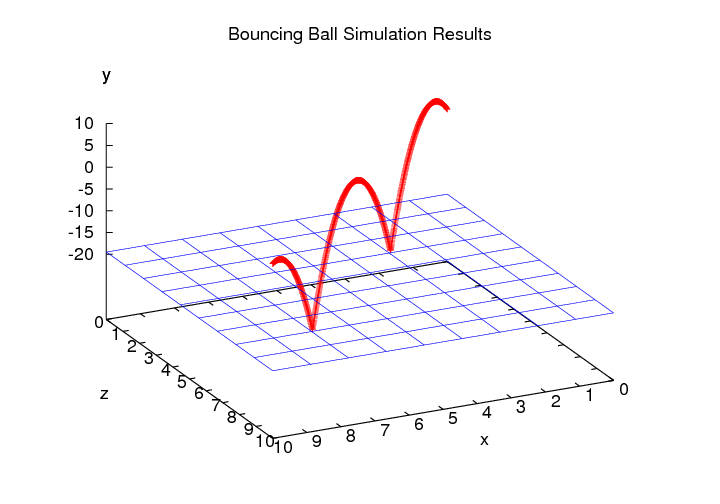
\includegraphics{gravity_plot.jpg}}
\end{center}
\caption{Trajectory of a ball bouncing under gravity with linear viscosity (from \texttt{gravity.py})} \label{fig:bouncy_ball}
\end{figure}

\subsection{Generating a bonded lattice of particles}

In the next example we will modify our bouncing ball script to replace the single particle with a bonded cube of particles. This serves to illustrate the three steps for generating an assembly of particles:

\begin{enumerate}
\item generating a block of unbonded particles,
\item creating bonds between neighbouring particles, and
\item specifying the type of interactions between bonded particle-pairs.
\end{enumerate}

\noindent 
The complete code-listing for this example is provided in Appendix~\ref{code}, entitled \texttt{grav\+i\+ty\_\+cube.py}. We will replace the code-fragment (in \texttt{gravity.py}) for creating a single particle with the code below. 

\subsubsection{Generating a block of unbonded particles}

ESyS-Particle provides four methods for generating a block of particles: 

\begin{itemize}
\item \texttt{SimpleBlock} -- generates a block of particles whose centres-of-mass reside on the vertices of a regular cubic lattice. This is the simplest configuration but is typically not the best choice for serious simulations since the particle-packing is not ideal (the porosity is very high).
\item \texttt{CubicBlock} -- generates a Face-Centred Cubic (FCC) lattice of particles with a dense packing arrangement. 
\item \texttt{HexagBlock} -- generates a Hexagonal Close Packing (HCP) of particles.
\item \texttt{RandomBoxPacker} -- generates a block of particles with radii randomly distributed in a specified range.
\end{itemize}

\noindent For illustrative purposes, we will use the \texttt{CubicBlock} in our example. The \texttt{SimpleBlock} and \texttt{HexagBlock} are implemented in the same manner. Generation of the block of random-sized particles is somewhat different and is covered in the next tutorial.

To begin using \texttt{CubicBlock} add the following line to the other import lines at the start of the code:

\begin{verbatim}
from esys.lsm.geometry import CubicBlock, ConnectionFinder
\end{verbatim}

The following code-fragment generates an FCC cubic block of particles and adds them to the simulation object:

\begin{verbatim}
cube = CubicBlock(dimCount=[6,6,6], radius=0.5)
cube.rotate(axis=Vec3(0,0,3.141592654/6.0),axisPt=Vec3(0,0,0))
sim.createParticles(cube)
\end{verbatim}

\noindent A \texttt{CubicBlock} object is instantiated via two arguments: \texttt{dimCount} and \texttt{radius}. \texttt{dimCount} is a three-element list specifying the number of particles to insert in each axis direction (in this case, the cube will comprise 6 particles per side). The \texttt{radius} of the particles is determined by the second argument. The physical dimensions of the \texttt{CubicBlock} are thus governed by the combination of the \texttt{radius} and the \texttt{dimCount} (in this case the cube will be $6\mathrm{m} \times 6\mathrm{m} \times 6\mathrm{m}$).

The second command (\texttt{cube.rotate(..)}) rotates the cube by 30 degrees about the Z-axis. This is done so the cube will first strike the floor on an angle rather than flat on one face. This should make the subsequent bounces a bit more interesting! The final command adds our cube of particles to the simulation object.

\subsubsection{Creation of inter-particle bonds}

By default the \texttt{CubicBlock} class creates an unbonded particle assembly. In order to construct a bonded particle assembly we must explicitly inform the simulation object that particles are to be bonded together. The following code-fragment achieves this:

\begin{verbatim}
sim.createConnections(
   ConnectionFinder(
      maxDist = 0.005,
      bondTag = 1,
      pList = cube
   )
)
\end{verbatim}

\noindent
The aim of this code is to construct a list of particle-pairs that are to be bonded together. The \texttt{ConnectionFinder} is an object that searches the list of particles provided as the \texttt{pList} argument (our \texttt{cube} in this case) looking for pairs of particles that are within a  specified distance (\texttt{maxDist}) of each other. The chosen distance in this case is $0.005$~m. Each pair of particles found will be added to a list and assigned a \texttt{bondTag} which we will use in the next section to specify the type of interactions between bonded particles.


\subsubsection{Specification of bonded-particle interactions}

Once we have inserted the block of particles into the simulation object and bonded the particles together, we must specify the type of interactions between bonded particles and initialise the interaction parameters. Once again, we utilise an \texttt{InteractionGroup} with an appropriate parameter set. For this example we will create non-rotational elastic bonds between bonded particles as specified in the \texttt{NRotBondPrms} parameter set:

\begin{verbatim}
bondGrp = sim.createInteractionGroup(
   NRotBondPrms(
      name = "sphereBonds",
      normalK = 10000.0,
      breakDistance = 50.0,
      tag = 1,
      scaling = True
   )
)
\end{verbatim}

\noindent 
\texttt{NRotBondPrms} contains five parameters: a bond \texttt{tag} specifying which bonded particles will undergo this interaction, a unique \texttt{name} for the interaction group, the elastic stiffness (\texttt{normalK}) of the bonds, a boolean (\texttt{scaling}) to specify whether to scale the stiffness with particle size, and a \texttt{breakDistance} specifying the separation distance that must be exceeded in order to break a bond between two particles. When a particle-pair exceeds the \texttt{breakDistance} the bond is removed and those two particles thereafter interact according to the interactions specified for unbonded particle pairs. In a later tutorial we will illustrate how to model elastic-brittle fracture of a bonded particle assembly. In this example we have chosen a very large \texttt{breakDistance} in order to prevent fracture of our cubic block when it bounces.

Modify \texttt{gravity.py} and replace the three lines that created the single particle with the code-fragments above, then run the simulation. This time you should obtain snapshots of a cube of particles bouncing off the table. Figure~\ref{fig:gravity_cube} provides a few snapshots from this simulation.

\begin{figure}
\resizebox{\textwidth}{!}{
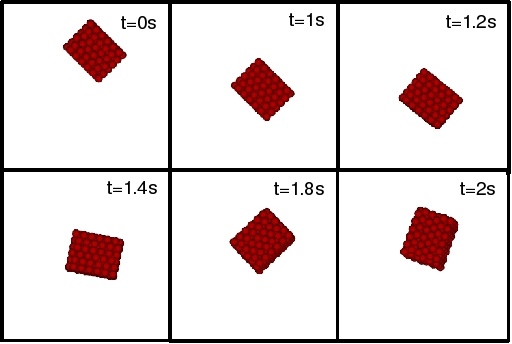
\includegraphics{gravity_cube_snaps.jpg}}
\caption{A sequence of snapshots of a bouncing cube of particles (from \texttt{grav\+i\+ty\_\+cube.py})} \label{fig:gravity_cube}
\end{figure}

It is instructive to note here that although we are using non-rotational spheres and interactions, the cube itself does rotate during the simulation. This is because forces between the wall and individual particles comprising the cube impart a torque to the cube as a whole when these forces do not point in the direction of the centre-of-mass of the entire cube. This is physically what we expect for this configuration and this fact can be exploited to simulate rotational dynamics without using the more computationally expensive particle-scale rotational interactions implemented in ESyS-Particle. The downside of this approach is that we must bond together a number of particles to represent an individual discrete entity in the simulation, thus increasing the total number of particles and simulation time. The decision as to which approach to use depends upon the scenario you wish to simulate. Some simulations of rotating, interacting entities do not require particle-scale rotational dynamics to achieve 
physically reasonable results.

\subsection*{What's next?}

In this section we learned how to add body forces (such as gravity and bulk viscosity) and simple walls to ESyS-Particle simulations. We also demonstrated how to bond particles together to simulate rigid bodies made out of an aggregate of spheres. The rotational dynamics observed for a cube of particles bouncing on a table arises simply by bonding the constituent particles with simple elastic bonds. The elastic bonds themselves are translational but when particles are clustered, bulk rotational dynamics (of the particle assembly) can be achieved.

The following tutorial builds upon the techniques learned in this section, introducing some new techniques for simulating two slightly more complicated scenarios: collapse of a pile of material under gravity and flow of loose granular material from a hopper or silo.  We will illustrate how to create blocks comprised of particles with variable radii, how to implement simple frictional interactions between unbonded particles, and how to exploit symmetries to improve simulation results without increasing the number of particles and hence the total computation time of simulations. We will also describe how to use triangle meshes to create walls with complicated shapes or containing holes. A hopper flow simulation will be used to illustrate how mesh walls are incorporated in ESyS-Particle simulations.

\chapter{Advanced Models}
\section{Slope failure \& hopper flow: variable particle sizes, friction \& mesh walls}

So far we have encountered examples of all the basic elements making up an ESyS-Particle simulation: a simulation object, particle assemblies, particle-particle interactions, body forces, walls and particle-wall interactions. Along the way we have learnt how to output simulation data to disk, make snapshots of particles in motion, and create re-usable \texttt{Runnables} to achieve user-defined functions during simulations. The aim of this and subsequent tutorials is to introduce a few more techniques commonly used in particle simulations including frictional interactions, brittle failure of elastic bonds, movement of walls, saving data using FieldSavers and the use of mesh walls to simulate complicated boundary geometries.

This tutorial uses slope failure and hopper flow as the motivation for the introduction of blocks comprised of particles of various sizes, frictional interactions between unbonded particles, a simple method to simulate frictional walls and the inclusion of mesh walls. We also discuss how symmetries in the problem to be solved can often be exploited to improve simulation results without greatly increasing computation time. Slope failure is an important problem in natural hazards (e.g.\ landslides), in handling of granular materials (e.g.\ forming piles of sand or grains) and in minerals processing (e.g.\ the stock-piling of ore in muckpiles). The study of hopper flow also plays its role in materials handling (e.g.\ grain storage in silos). Along the way, the examples in this tutorial will illustrate some of the key features of sand-piles, as well as introducing a few more ESyS-Particle tricks and techniques.

\subsection{Splash-down: collapse of a block of particles with variable sizes}

Until this point we have dealt predominantly with assemblies of particles with a constant particle radius. Experience has shown that often the use of uniform particle sizes and regular particle arrangements introduces artifacts such as preferential movement along lattice planes. A simple way to remove such artifacts and to model more realistic granular materials is to use particle assemblies in which the positions and radii of particles are selected randomly. ESyS-Particle provides a simple mechanism for constructing a rectangular block of particles with random positions and radii. The following code fragment achieves this:

\begin{verbatim}
geoRandomBlock = RandomBoxPacker (
   minRadius = 0.2000,
   maxRadius = 0.5000,
   cubicPackRadius = 2.2000,
   maxInsertFails = 1000,
   bBox = BoundingBox(
      Vec3(-5.0000, 0.0000,-5.0000),
      Vec3(5.0000, 10.0000, 5.0000)
   ),
   circDimList = [False, False, False],
   tolerance = 1.0000e-05
)
geoRandomBlock.generate()
geoRandomBlock_particles = geoRandomBlock.getSimpleSphereCollection()
sim.createParticles(geoRandomBlock_particles)
\end{verbatim}

To construct a random block of particles, we first create a \texttt{RandomBoxPacker} by providing a number of parameters defining the range of particle radii (\texttt{minRadius} and \texttt{maxRadius}), the geometry of the block to fill with particles (\texttt{bBox}) and some additional parameters related to the algorithm used to fill the block. We will discuss the particle packing algorithm in a few moments. The example above will construct a cube 10 metres on a side containing particles whose radii range from 0.2 metres to 0.5 metres. One corner of the cube will be located at $(X,Y,Z) = (-5,0,-5)$. 

\subsubsection{Algorithm for packing particles into a prescribed region}

The \texttt{RandomBoxPacker} and some other ESyS-Particle \texttt{Packer} modules make use of an iterative, geometrical space-filling algorithm to insert particles within a prescribed volume (a rectangular prism in the case of \texttt{RandomBoxPacker}). The algorithm may be summarised as follows:

\begin{enumerate}
\item Insert a number of seed particles at random locations within the volume ensuring they do not overlap.
\item Identify 4 adjacent particles 
\begin{enumerate}
\item compute the centroid of the tetrahedron defined by the 4 particles 
\item compute the radius of a particle that touches all 4 particles
\item if the radius of that particle is within the specified range and it is entirely within the prescribed volume, insert the particle
\end{enumerate}
\item Repeat step 2 until the number of failed insertion attempts reaches \texttt{maxInsertFails}
\end{enumerate}

\noindent
The \texttt{tolerance} parameter defines what is meant by \emph{touching} in the algorithm above. If particles overlap by less than the prescribed \texttt{tolerance}, they are said to be touching. The \texttt{cubicPackRadius} is a parameter for setting up the neighbours table used to track relative locations of adjacent particles. The optimal value for this is approximately $2.2 \times$ \texttt{maxRadius}. \texttt{circDimList} informs the packing algorithm of any circular (or periodic) boundaries so particles will be fitted together along these boundaries rather than being fitted to straight walls.

This algorithm for filling a volume with spherical particles has some distinct advantages over some other methods but also some limitations. The algorithm requires no equilibriation simulation like some dynamical methods (e.g.\ expanding particle algorithms) to achieve a close packing of relatively low porosity. The algorithm is also easily adapted for filling quite arbitrary-shaped volumes, a feature exploited in the \texttt{GenGeo} add-on library for ESyS-Particle (which we will discuss later). On the downside, the user has little control over the final distribution of particle sizes (apart from specifying the range of sizes). Experience as shown that for a broad range of sizes (e.g.\ $[0.1, 1.0]$) the final particle size distribution is a power-law. For a narrow range of sizes (e.g. $[0.4,0.6]$) the size distribution is approximately a uniform random distribution. 

\subsubsection{Simulating collapse of a cube of unbonded particles}

The aim of this example is to demonstrate the simulation of collapse of a cube of unbonded particles under the action of gravity. Suppose one had a container of loose, dry powder (such as sand or dirt) upturned on a table. When one lifts the container, one expects the powder to fall outwards forming a pile. Rather than going straight to a complete simulation of the process, we will progress in a number of stages so as to illustrate some important points about both the dynamics of sand-piles and about tricks that can be applied to simulate phenomena realistically using the Discrete Element Method.  

Write an ESyS-Particle script comprised of a cube of particles sitting atop a wall representing the table. Implement simple elastic repulsion between the particles, and between particles and the wall. In addition, implement gravity and viscosity, and add a \texttt{Runnable} to store snapshots every 1000 timesteps. Run the simulation for 50000 timesteps with a timestep increment of $10^{-4}$. If you need some help, refer to the \texttt{slope\_fail.py} code-listing in Appendix~\ref{code}. Once you have run the simulation, you should have a sequence of snapshots similar to those illustrated in Figure~\ref{fig:slope_fail_pics}. 

The most striking feature of the simulation results is the non-existence of a pile at the end of the simulation. In fact, a movie of the simulation snapshots looks remarkably like a fluid splashing down on the table (hence the name of this example: Splash-down). The reason for the discrepancy between the simulated results and our expected results lies in the simplified physics we have implemented in the model. It is well-known that the formation of sand-piles is governed by frictional interactions between the sand grains. Indeed the steepness of the pile (known as the \emph{angle of repose}) is directly related to the coefficient of inter-granular friction. In the next example we will attempt to improve our model by incorporating frictional interactions between unbonded particles.

\begin{figure}
\resizebox{\textwidth}{!}{
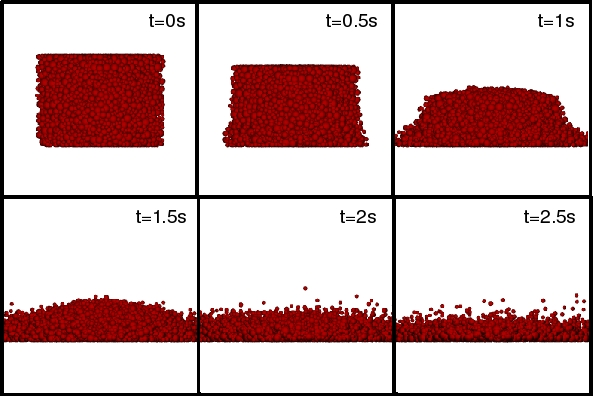
\includegraphics{slope_fail_snaps.jpg}}
\caption{A sequence of snapshots from a frictionless slope collapse simulation (from \texttt{slope\_\+fail.py})} \label{fig:slope_fail_pics}
\end{figure}

\subsection{Sand-piles: adding frictional interactions}

\subsubsection{Frictional interactions between unbonded particles}

As we saw in the previous example, the use of simple elastic repulsion between particles is insufficient to model formation of a sand-pile. The reason for this is postulated to be the lack of frictional interactions between the particles. In this example we will replace the \texttt{NRotElastic} Interaction Group with a new Interaction Group (called \texttt{NRotFriction}) incorporating both elastic repulsion and frictional resistance between touching particles. The following code-fragment illustrates how to incorporate frictional interactions in a simulation:

\begin{verbatim}
sim.createInteractionGroup (
   NRotFrictionPrms (
      name = "friction",
      normalK = 1000.0,
      dynamicMu = 0.6,
      shearK = 100.0,
      scaling = True
   )
)
\end{verbatim}

\noindent
In addition to the \texttt{name}, \texttt{normalK} and \texttt{scaling} parameters with which we are already familiar, \texttt{NRot\+Fric\+tionPrms} also requires two more parameters. The first parameter (\texttt{dynamicMu}) defines the coefficient of friction for touching particles whilst the second parameter (\texttt{shearK}) defines the shear stiffness at the contact point. When two particles first touch, a shear spring is created at the contact point. Forces from surrounding particles will cause the two particles to commence sliding past one-another with the shear spring resisting the motion. When the shear force exceeds the normal force multiplied by the coefficient of friction, dynamic sliding commences (as the maximum shear force is governed by the normal force and the friction coefficient). This is a simple yet effective method to simulate both static deformation at frictional contacts and dynamic frictional sliding. 

Change your \texttt{slope\_fail.py} script and replace the \texttt{NRotElasticPrms} interaction group with the code-fragment above (c.f.\ \texttt{slope\_friction.py} in Appendix~\ref{code}). Re-run the simulation and study the snapshots carefully. You should obtain a snapshot sequence similar to that of Figure~\ref{fig:slope_friction_pics}. My guess is that you will still be a little disappointed with the results. Although a pile begins to form in the early stages of the simulation, the pile eventually collapses (albeit a bit later than in the first example). Whilst the inter-particle friction has clearly had an impact, collapse of the pile is inevitable because the table is frictionless. To maintain the pile, we require frictional interactions between the particles and the table also. In the next example we will demonstrate a way to simulate frictional walls. After that we will discuss how often symmetry in the problem of interest can be exploited to produce more useful results without increasing the total 
number of particles in a simulation.

\begin{figure}
\resizebox{\textwidth}{!}{
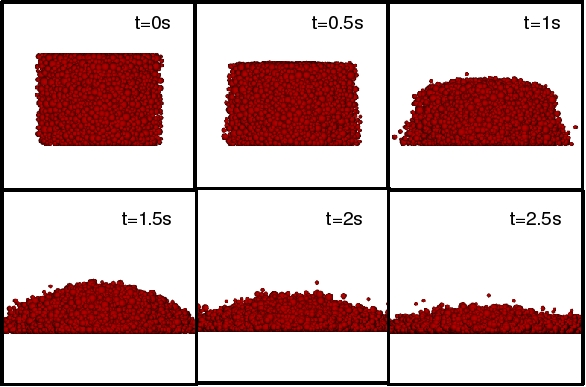
\includegraphics{slope_friction_snaps.jpg}}
\caption{A sequence of snapshots of slope collapse with frictional particles (from \texttt{slope\_\+fric\+tion.py})} \label{fig:slope_friction_pics}
\end{figure}

\subsubsection{Frictional interactions between particles and walls}

As we saw in the previous example, adding friction between particles certainly helps to form sand-piles but the lack of friction between particles and the table means the pile soon collapses. Once particles hit the table they slide away on the frictionless surface rather than remaining as support for particles rolling down on top. What we need is a frictional surface representing the table-top. At the time of writing this tutorial, ESyS-Particle has no Interaction Group specifically for frictional interactions between particles and walls. Consequently we need to think a little laterally to model a frictional surface.

One way would be to make the wall entirely out of a slab of stationary particles that interact with the falling particles via a \texttt{NRotFriction} interaction. I'll leave it as an exercise to try that yourself. Another alternative is to attach particles at the base of the cube to the wall using the \texttt{NRotBondedWall} interaction group. Particles attached to the wall will be constrained to remain in place, oscillating around a point if large forces are applied by surrounding particles. The main reason for choosing this approach is to demonstrate another useful feature of ESyS-Particle: tagging of groups of particles so we selectively apply interactions to those particles. This is a handy feature that will be useful in a number of different scenarios.

We aim to make use of the \texttt{NRotBondedWall} Interaction Group to bond particles to the wall with unbreakable elastic bonds. The code fragment for implementing such interactions is as follows:

\begin{verbatim}
sim.createInteractionGroup (
   NRotBondedWallPrms (
      name = "floor_bonds",
      wallName = "floor",
      normalK = 10000.0,
      particleTag = 12321
   )
)
\end{verbatim}

\noindent
The first three parameters should now be familiar. The fourth parameter (\texttt{particleTag}) specifies the tag of particles that will undergo bonded elastic interactions with the wall denoted by \texttt{wallName}. All other particles that touch the wall will undergo unbonded elastic repulsion, just like previous examples. 

In order to bond specific particles to the wall, we need to assign a specific tag to those particles prior to inserting them into the simulation object. We can do this by individually inserting each particle within our random cube of particles and checking as we go whether those particles are close to the wall or not. The following code fragment achieves this:

\begin{verbatim}
for pp in geoRandomBlock_particles:
   centre = pp.getPosn()
   radius = pp.getRadius()
   Y = centre[1]
   if (Y < 1.1*radius):
      pp.setTag(12321)       # tag particles nearest to the floor
   sim.createParticle(pp)    # add the particle to the simulation object
\end{verbatim}

\noindent
Rather than simply inserting the \texttt{geoRandomBlock\_particles} directly into the simulation object with a call to \texttt{sim.createParticles(..)}, we read each particle in the list and check whether its centre is within $1.1 \times$ the radius of that particle. If so, we set the tag of the particle to $12321$, denoting this particle as one to bond to the wall. Finally a call to \texttt{sim.createParticle(..)} adds each particle to the simulation object.

Go ahead and modify \texttt{slope\_friction.py} to include the changes above. Remember to replace the \texttt{NRotElasticWall} Interaction Group with the \texttt{NRotBondedWall} Interaction Group. The complete code-listing for the modified script is called \texttt{slope\_\+fric\+tion\_\+floor.py} in Appendix~\ref{code}. Having made the necessary modifications, execute the simulation and record some snapshots. All being well, you should see a sequence of snapshots like Figure~\ref{fig:slope_friction_floor_pics}. Hurray! Finally we have simulated the formation of a sandpile, albeit only above the base of the original cube. A lot of particles still flowed away due to the frictionless surrounding area. 

Whilst one may argue this simulation is still some ways from the scenario we hoped to simulate, we have learnt quite a bit about both sand-piles and some of the features of ESyS-Particle in the process. The results of this simulation demonstrate that by bonding particles to walls we can simulate a rough frictional surface quite effectively (and quite simply). The simulation also further demonstrates that a sand-pile requires a frictional floor in order to hold itself up. Any particles rolling down outside the base of the original cube just slide away and cannot support the weight of particles falling down from above. Of course, we would much prefer to be able to keep more of the particles within the sand-pile rather than losing more than half of them from the pile. The next example achieves this to some extent and, in the process, introduces a technique of great utility in Discrete Element Modelling - the use of symmetry in the problem of interest to reduce the number of particles needed to simulate a 
phenomenon. 

\begin{figure}
\resizebox{\textwidth}{!}{
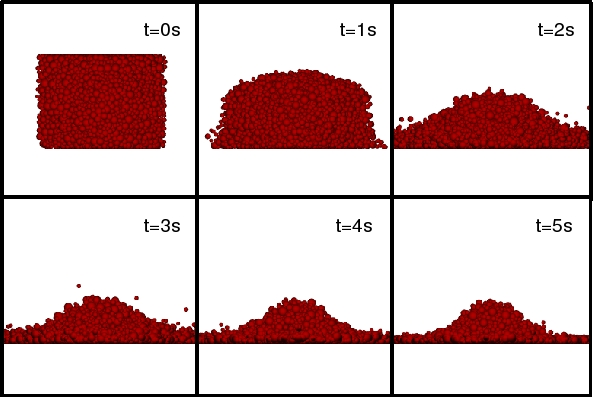
\includegraphics{slope_friction_wall_snaps.jpg}}
\caption{A sequence of snapshots of slope collapse with frictional particles and a frictional floor (from \texttt{slope\_friction\_floor.py})} \label{fig:slope_friction_floor_pics}
\end{figure}

\subsubsection{Making use of symmetry to improve simulation results}

Often the physical phenomenon one wishes to model contains geometrical symmetries that can be exploited to improve simulation results without needing to increase the total number of particles. For example, in our sand-pile simulations, the particles are initially arranged in a cubic volume which has three symmetry axes parallel with the sides of the cube. The final sand-pile is approximated by a cone which has circular symmetry around the (vertical) axis of the cone. In order to model the transformation of the cubic volume of particles into a conical pile, we really don't need to model the entire volume due to these inherent symmetries. A perfectly reasonable solution would be to model only one quarter of the cube collapsing to form one quarter of a cone. We can then rotate the final solution about the symmetry axis to obtain a reasonable representation for the final sandpile shape. The advantage is that we can model the process at higher resolution without increasing the total number of particles (and hence 
the time taken to run the simulation).

One needs to exercise some caution however to ensure that the physics along symmetry cut-planes is accurately modelled. Typically the dynamics either side of a symmetry cut-plane are the mirror image of each other, known as even symmetry. To achieve this, in most cases the use of frictionless walls along cut-planes achieves the desired result. To see how a quarter-symmetry simulation works, make the following modifications to your previous script (\texttt{slope\_friction\_floor.py}):

\begin{enumerate}
\item Add a wall located at $(X,Y,Z) = (-5,0,0)$ with a normal in the positive X-direction (i.e. $\hat{n} = (1,0,0)$). This wall will be known as the \texttt{left\_wall}. 
\item Add a second wall located at $(X,Y,Z) = (0,0,-5)$ with a normal in the positive Z-direction (i.e. $\hat{n} = (0,0,1)$). This wall will be known as the \texttt{back\_wall}. 
\item Insert two new \texttt{NRotElasticWall} Interaction Groups, one for each of the new walls.
\end{enumerate}

\noindent
Refer to \texttt{slope\_friction\_walls.py} in Appendix~\ref{code} if you are unsure how to do these steps. 

When completed, run your simulation for 100000 timesteps and record snapshots every 1000 timesteps. The results should be similar to those of Figure~\ref{fig:slope_friction_walls_pics}. Notice that we now have simulated formation of a pile that is almost twice as high as the previous example albeit we have only modelled one quarter of the sand-pile. Without increasing the number of particles we have now simulated the formation of a pile that has a basal area effectively four times that of the previous example. Although some particles still slide away on the frictionless floor, we have improved the spatial resolution of our sand-pile model quite considerably without sacrificing computation time. 

\begin{figure}
\resizebox{\textwidth}{!}{
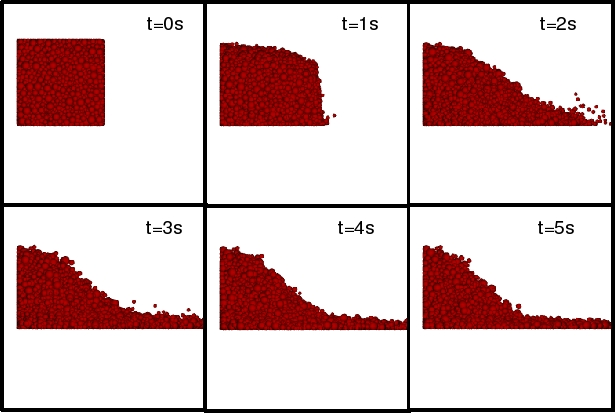
\includegraphics{slope_friction_quarter_snaps.jpg}}
\caption{A sequence of snapshots of slope collapse utilising quarter symmetry (from \texttt{slope\_friction\_walls.py})} \label{fig:slope_friction_walls_pics}
\end{figure}

In many instances exploiting symmetries in the problem at hand can greatly increase the accuracy of results without greatly increasing computation time. However one must be careful to avoid artifacts induced by potentially inaccurate boundary conditions along symmetry cut-planes. In some cases other problem constraints demand that large numbers of particles must be used. In those instances, exploiting symmetry may be the only option. Later we will encounter another useful technique for reducing problem sizes without greatly impacting simulation results - the use of periodic boundary conditions to simulate models that are effectively semi-infinite in one coordinate direction. 

\subsection{Hopper flow: Using quarter symmetry and mesh walls}

Now that you've discovered the joys of slope collapse, there are really only a couple of steps to take this simulation and use it to study hopper flows. The flow of material in silos encounters many problems in the real world. These include rat-holing, stalling of flow around the exit, uneven draw profiles and unexpected segregation of finer material to name a few. The study of granular flow is a dynamic problem requiring many timesteps of simulation. In the previous section we learnt how to use quarter symmetry to improve simulation performance; hopper flow is another application that benefits from the use of symmetry. By using quarter symmetry planes around an exit point and modelling those planes using frictionless walls we can simulate models representative of hoppers of much larger capacity.

\subsubsection{The mesh wall file format}

So far we have only used planar walls in our simulations. Planar walls, by their definition, are infinite in length, making it difficult to simulate problems that require complex wall shapes or walls with holes. Mesh walls overcome this problem but are slightly more complicated to implement in simulations. ESyS-Particle uses a triangulated mesh format to define piecewise segments of a wall. Generation of these meshes can be done through most CAD packages but require a little work to convert into the ESyS-Particle mesh format. An example mesh file is shown below for an "L" shaped floor mesh that we will use in the upcoming example:

\begin{verbatim}
Triangle
3D-Nodes 6
 0  0 0  -5.0  0.0   0.0
 1  1 0  -5.0  0.0   5.0
 2  2 0   0.0  0.0  -5.0
 3  3 0   0.0  0.0   0.0
 4  4 0   5.0  0.0  -5.0
 5  5 0   5.0  0.0   5.0

Tri3 4
 0  0  0  3  1
 1  0  1  3  5
 2  0  5  3  4
 3  0  3  2  4
\end{verbatim}

The mesh file commences with a format header \texttt{Triangle}; the number after \texttt{3D-\+Nodes} specifies how many nodal points exist in the mesh followed by the specification of locations of these points in the format:
\begin{verbatim}
ID Dummy Tag X Y Z
\end{verbatim}

The number after \texttt{Tri3} specifies how many triangle elements exist in the mesh. Normals of triangles are considered to be pointing out of the page using an                                                         anti-clockwise piecewise specification, regarding which see Figure~\ref{fig:trimesh_normal}. The tri-elements link the nodes in the following manner:
\begin{verbatim}
ID Tag Point1 Point2 Point3
\end{verbatim}

\begin{figure}
\begin{center}
\resizebox{3in}{!}{
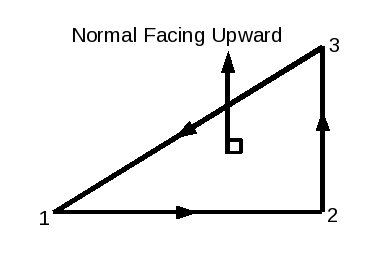
\includegraphics{trimesh_normal.jpg}}
\end{center}
\caption{Specification of mesh nodes for wall normals} \label{fig:trimesh_normal}
\end{figure}

\subsubsection{Using mesh walls in hopper flow simulations}

Save the triangle mesh wall specification above in a file called \texttt{floorMesh.msh}. We can now read the mesh wall into a simulation object using the following code fragment:

\begin{verbatim}
sim.readMesh(
   fileName = "floorMesh.msh",
   meshName = "floor_mesh_wall"
)
\end{verbatim}

The variable \texttt{meshName} will be used later to create an interaction group between the particles and the mesh wall, just as we do for planar walls. Let's get started by editing our \texttt{slope\_friction\_walls.py} script to replace the bonded floor with a mesh wall:

\begin{enumerate}
\item Replace the current \texttt{floor} wall code with the above code fragment to import the mesh wall instead.
\item Replace the current interaction group \texttt{floor\_bonds} with the following interaction group for mesh walls:

\begin{verbatim}
sim.createInteractionGroup (
   NRotElasticTriMeshPrms (
      name = "floorWall_repell",
      meshName = "floor_mesh_wall",
      normalK = 1.0000e+04
   )
)
\end{verbatim}

This interaction group creates a non-rotational elastic interaction that repels  particles that make contact with the mesh wall, essentially just like a planar wall. We also wish to constrain our hopper so that particles may only exit via the hole in the mesh wall. We can do this by adding front and right walls to our simulation, in addition to the left and back walls added in the previous example:
\item Add a third wall located at $(X,Y,Z) = (5,0,0)$ with a normal in the negative X-direction (i.e. $\hat{n} = (-1,0,0)$). This wall will be known as the \texttt{right\_wall}.
\item Add a fourth wall located at $(X,Y,Z) = (0,0,5)$ with a normal in the negative Z-direction (i.e. $\hat{n} = (0,0,-1)$). This wall will be known as the \texttt{front\_wall}.
\item Insert two more \texttt{NRotElasticWall} Interaction Groups, one for each of the new walls.
\item Finally we will change the tagging of the particles for visualisation purposes. Change the tagging code fragment from the previous example to the following: code to the fragment below will colour the particles in layers of 2m in the Y direction:

\begin{verbatim}
#add particles to simulation one at a time,
#tagging those in layers of 2m
for pp in geoRandomBlock_particles:
   centre = pp.getPosn()
   Y = centre[1]
   if (int(Y%4) < 2):
      pp.setTag(1) # layer 1
   else:
      pp.setTag(2) # layer 2
   sim.createParticle(pp) # add particle to the simulation object
\end{verbatim}

The new tagging code will tag particles with one of two different tags, in layers of 2m in the vertical Y-direction.  As mentioned before, particle tags can be used for a range of simulation-related functions.  In this example we have used tagging to identify the initial location of particles in the vertical direction. This makes it easier for us to visualise the flow of particles later.
\end{enumerate}

Congratulations, you have now made all of the changes to the code required to do a hopper flow simulation. Run your code and you should expect something as in Figure~\ref{fig:hopper_flow}. If not, refer to \texttt{hopper\_flow.py} in Appendix~\ref{code}.

As you have seen, mesh walls are a powerful and flexible feature of ESyS-Particle that allow complex shapes and interactions to be simulated. Discussing the model above, two unrealistic simplifications have been used that results in hopper flow dynamics somewhat different to that of real hoppers. Firstly, we use non-rotational particles as our granular media. This consequence of this is that friction between particles is higher than reality; particles are not able to roll over one another. The consequent higher bulk friction results in more frequent rat-holing or stalling of flow around the outlet. The second simplification is the use of a frictionless mesh wall as the base of the hopper. As with the slope collapse example in the previous section, particles can freely slide along the base surface as there is no shear/frictional component to the interaction. This will result in a wider flow pattern than usual, with particles sliding towards the outlet more easily. A more realistic simulation would include 
frictional interactions at the base of the hopper, perhaps by using the bonding technique introduced in the example above.

\begin{figure}
\begin{center}
\resizebox{2.5in}{!}{
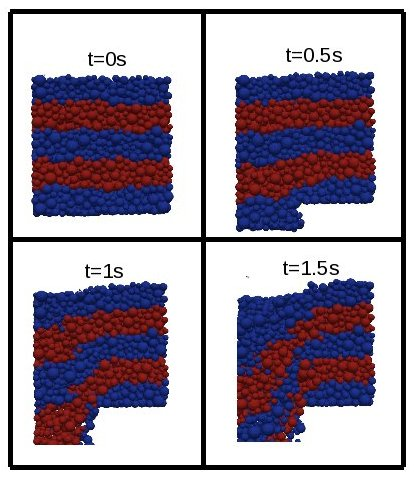
\includegraphics{hopper_flow.jpg}}
\end{center}
\caption{Hopper flow using a mesh base in quarter symmetry (from \texttt{hopper\_flow.py})} \label{fig:hopper_flow}
\end{figure}

\subsection*{What's next?}

This chapter has introduced a number of new features of ESyS-Particle as well as some tricks and hints for obtaining more realistic simulation results without greatly increasing the mathematical complexity of the model. We have seen how to create a block of variable-sized particles at random locations. This avoids unphysical dynamics often encountered when using particles of equal size in regular crystalline packing arrangements. Techniques for tagging particles and bonding these tagged particles to walls, as well as introduction of mesh walls, provide methods to simulate complex boundary conditions including frictional walls of a variety of shapes. For problems that allow it, the use of symmetry-planes can increase the resolution of simulation results without greatly increasing the computation time.  

In the following tutorial we examine elastic-brittle failure of rock samples under uniaxial compression. Simulations of uniaxial compression are particularly important in Discrete Element Modelling, providing a way to calibrate numerical models so that the macroscopic physical properties (such as elastic moduli and failure strength) match those of real rocks. In order to simulate rock breakage under uniaxial loads, we will need to implement movable walls and introduce rotational cementatious elastic-brittle bonds. We will also examine the use of \texttt{FieldSavers} to selectively store simulation data such as wall forces, total strain energy and the number of broken bonds. Particular attention will be paid to how one may calibrate DEM simulations to achieve desired macroscopic properties. 
%This will lead on to the topic of the following tutorial: measurement of the macroscopic friction angle of loose granular materials via shear cell simulations.

\newpage
\section{Uniaxial compression simulations: moving walls, model calibration and \texttt{FieldSavers}}

Quasi-static uniaxial compression of rock samples is a common laboratory technique for measuring the macroscopic properties of rocks such as Young's modulus, Poisson's ratio and the unconfined compressive strength. In uniaxial compression experiments, a sample of rock is slowly compressed by a piston until failure occurs. By measuring the force applied to the sample and the strain, one can measure the Young's modulus of the rock sample. The peak stress at which failure of the sample occurs is known as the Unconfined Compressive Strength (UCS), an important measure of the strength of rocks. 

In this tutorial we will describe how to perform uniaxial compression simulations using ESyS-Particle. Such simulations provide a means to measure the equivalent macroscopic properties of synthetic rock samples and are an important tool for calibrating Discrete Element models. When discussing calibration it is important to distinguish between the microphysical parameters defining interaction laws (e.g.\ elastic stiffnesses, coefficients of friction, etc.) and the macroscopic elastic properties (Young's modulus, macroscopic friction angle, etc.). The later are a function not only of the microphysical parameters, but also the geometrical properties of the network of bonded and unbonded interactions within the particle assembly. There is often no known analytical relationship between the microphysical parameters and the macroscopic properties (except in special cases of regular packings of equal-sized particles). To overcome this, it is common procedure to conduct a series of uniaxial compression simulations to 
tune the microphysical parameters until desired macroscopic properties are obtained.

To simulate rock breakage under compressive loads, we will need to introduce a number of new ESyS-Particle techniques. These include:

\begin{enumerate}
\item implementation of cementatious (rotational) elastic-brittle bonds and rotational friction interactions,
\item moving walls via a \texttt{Runnable}, and
\item selective storage of simulation data using \texttt{FieldSavers}.
\end{enumerate}

\noindent
Rather than incrementally building upon previous examples, this tutorial is written stand-alone, containing all code-fragments needed to implement uniaxial compression simulations. We will also discuss how to measure macroscopic elastic properties using simulation results.

\subsection{Uniaxial compression simulations}

In this example we will discuss how to implement a uniaxial compression simulation using ESyS-Particle. The model will consist of a rectangular prism of particles sandwiched between two piston walls which will be compressed at constant speed. We will utilise \texttt{FieldSavers} to monitor the positions of, and forces acting on, the walls, as well as the total strain energy stored in bonds between particles and the number of broken bonds. These simulation data will then be used to measure the macroscopic elastic properties of the particle model. Full code-listings for uniaxial compression simulations are available in Appendix~\ref{code}.

%Since calibrating microscopic model parameters to achieve desired macroscopic elastic properties is the main objective, we will take more care in this tutorial to choose realistic parameter values. To do this requires that we choose a system of units of measure that is self-consistant and practical. ESyS-Particle is coded so that the choice of units of measure is arbitrary. The user may decide whether to use measurement units in MKS (metres, kilograms and seconds), CGS (centimetres, grams and second) or another system defining the units of Length, Mass and Time. No assumptions are made within ESyS-Particle a priori about the units of measure except that by default, particles have a density equal to 1.0. In the following example we will explicitly set the density of particles. 

%For the following example, we will use millimetres, Newtons and milliseconds as our fundamental units of measure. These are selected primarily for convenience. Laboratory uniaxial compression tests typically utilise rock samples approximately 50mm in diameter and around 100mm long. The Young's moduli of rocks are of order $40-80$GPa and peak strengths are between 100MPa and 250MPa. By using millimeters and Newtons as fundamental units, stresses in our simulation will be in units of N/mm/mm, which is equivalent to MPa. Similarly, by choosing milliseconds as out third unit of measure, velocities will be reported in m/sec and masses will be measured in grams. There is no reason why we could not have used MKS units in these simulations, but this selection just makes measuring results easier for calibration purposes. 

\subsubsection{Initialising the simulation object}

Every ESyS-Particle simulation requires a \texttt{LsmMpi} simulation object. This object serves as a container to which we can add particles, walls, interactions and other modules for storing data or moving walls. The following code-fragment loads the ESyS-Particle Python modules and initialises the simulation object:

\begin{verbatim}
#import the appropriate ESyS-Particle modules:
from esys.lsm import *
from esys.lsm.util import *
from esys.lsm.geometry import *

#instantiate a simulation object:
sim = LsmMpi (numWorkerProcesses = 1, mpiDimList = [1,1,1])

#initialise the neighbour search algorithm:
sim.initNeighbourSearch (
   particleType = "RotSphere",
   gridSpacing = 5.0000,
   verletDist = 0.08000
)

#set the number of timesteps and timestep increment:
sim.setNumTimeSteps (250000)
sim.setTimeStepSize (1.0000e-06)

#specify the spatial domain for the simulation
domain = BoundingBox(Vec3(-20,-20,-20), Vec3(20,20,20))
sim.setSpatialDomain (domain)
\end{verbatim}

\noindent
Most of these commands should now be familiar from previous tutorials. We first import a number of useful ESyS-Particle modules and create an instance of the \texttt{LsmMpi} simulation object. Whilst initialising the neighbour search algorithm, we specify that particles are of type \texttt{RotSphere} (unlike previous examples where we used \texttt{NRotSphere} particles). Subsequently we set the number of timesteps, the timestep size and the extents of the spatial domain. The simulation object is now initialised and ready to insert particles, interactions, walls, etc.

\subsubsection{Creating a block of variable-sized particles}
\label{sec:block_in_sim}

Having initialised the simulation object, we need to insert particles and bond them together. For rock breakage simulations, the best results are obtained using blocks of particles with variable radii and random locations. We will use the \texttt{RandomBoxPacker} first encountered in the previous tutorial:

\begin{verbatim}
#create a prism of spherical particles:
geoRandomBlock = RandomBoxPacker (
   minRadius = 0.400,
   maxRadius = 2.0000,
   cubicPackRadius = 2.2000,
   maxInsertFails = 5000,
   bBox = BoundingBox(
      Vec3(-5.0000, 0.0000,-5.0000),
      Vec3(5.0000, 20.0000, 5.0000)
   ),
   circDimList = [False, False, False],
   tolerance = 1.0000e-05
)
geoRandomBlock.generate()
geoRandomBlock_particles = geoRandomBlock.getSimpleSphereCollection()

#add the particles to the simulation object:
sim.createParticles(geoRandomBlock_particles)

#bond particles together with bondTag = 1:
sim.createConnections(
   ConnectionFinder(
      maxDist = 0.005,
      bondTag = 1,
      pList = geoRandomBlock_particles
   )
)
\end{verbatim}

\noindent
This code-fragment generates a rectangular prism of particles whose radii lie in the range $[0.4, 2.0]$~mm. The prism is $10 \times 20 \times 10$~mm in size with the centre of the base at the origin. The final command adds the prism of particles to the simulation object. For more information about the \texttt{RandomBoxPacker} and the ESyS-Particle particle packing algorithm, please refer to the previous tutorial. The last section of this code-fragment uses a \texttt{ConnectionFinder} to find pairs of particles within a distance of 0.005~mm of each other. Each particle pair is tagged with a \texttt{bondTag} that we will use to specify the type of interactions between bonded particles below. We first encountered the \texttt{ConnectionFinder} in \texttt{gravity\_cube.py} when we created a bonded cube of particles to bounce on the floor.

\subsubsection{Adding walls to the simulation object}

Next we need to add two walls to the simulation object. These walls will serve as pistons for compressing the rock sample. We will add one wall below the sample (the \texttt{bottom\_wall}) and another atop the sample (the \texttt{top\_wall}):

\begin{verbatim}
#create a wall at the bottom of the model:
sim.createWall (
   name = "bottom_wall",
   posn = Vec3(0.0000, 0.0000, 0.0000),
   normal = Vec3(0.0000, 1.0000, 0.0000)
)

#create a wall at the top of the model:
sim.createWall (
   name = "top_wall",
   posn = Vec3(0.0000, 20.0000, 0.0000),
   normal = Vec3(0.0000, -1.0000, 0.0000)
)
\end{verbatim}

\noindent
Simply adding walls to the simulation object is insufficient. We must also define interactions between the walls and particles. For basic uniaxial compression simulations, repulsive elastic interactions are sufficient. If we were interested in tensile loading, we would need to bond the walls to particles at the base and top of the model. Bonding walls to particles was covered in the previous tutorial. For now, the following particle-wall interactions are all that are required:

\begin{verbatim} 
#specify elastic repulsion from the bottom wall:
sim.createInteractionGroup (
   NRotElasticWallPrms (
      name = "bottom_wall_repel",
      wallName = "bottom_wall",
      normalK = 100000.0
   )
)

#specify elastic repulsion from the top wall:
sim.createInteractionGroup (
   NRotElasticWallPrms (
      name = "top_wall_repel",
      wallName = "top_wall",
      normalK = 100000.0
   )
)
\end{verbatim} 

\noindent
These two code-fragments specify elastic repulsion from the \texttt{bottom\_wall} and \texttt{top\_wall}. Each Interaction Group is assigned a unique name that can be used to selectively store various data about interactions using \texttt{FieldSavers}. Elastic repulsion of particles from walls requires specification of a single microphysical parameter, the elastic stiffness (\texttt{normalK}). For this simulation we set the elastic stiffness equal to $100000$~N/mm.

%In the next section we will discuss how to rescale from simulation units to real units in the context of measuring macroscopic elastic properties. 

\subsubsection{Rotational bonds and frictional interactions}

In previous examples we have encountered two types of particle interactions: \texttt{NRotElastic} and \texttt{NRotFriction} interactions. Both of these interactions are designed for particles with only three (translational) degrees of freedom (known as \texttt{NRotSpheres}) and are suitable for granular flow of individual particles or aggregates. To simulate elastic-brittle failure of rocks, more sophisticated particle-pair interactions are required. In particular, we require particle-pair interactions that incorporate both translational and rotational degrees of freedom. As illustrated in Figure~\ref{fig:rot_bond_diagram}, two bonded particles may undergo normal and shear forces, as well as bending and twisting moments. Bonds designed to impart such forces and moments are known as cementatious bonds (or in ESyS-Particle parlance \texttt{BrittleBeamPrms} interactions). 

\begin{figure}
\begin{minipage}{3in}
\begin{center}
\resizebox{2in}{!}{
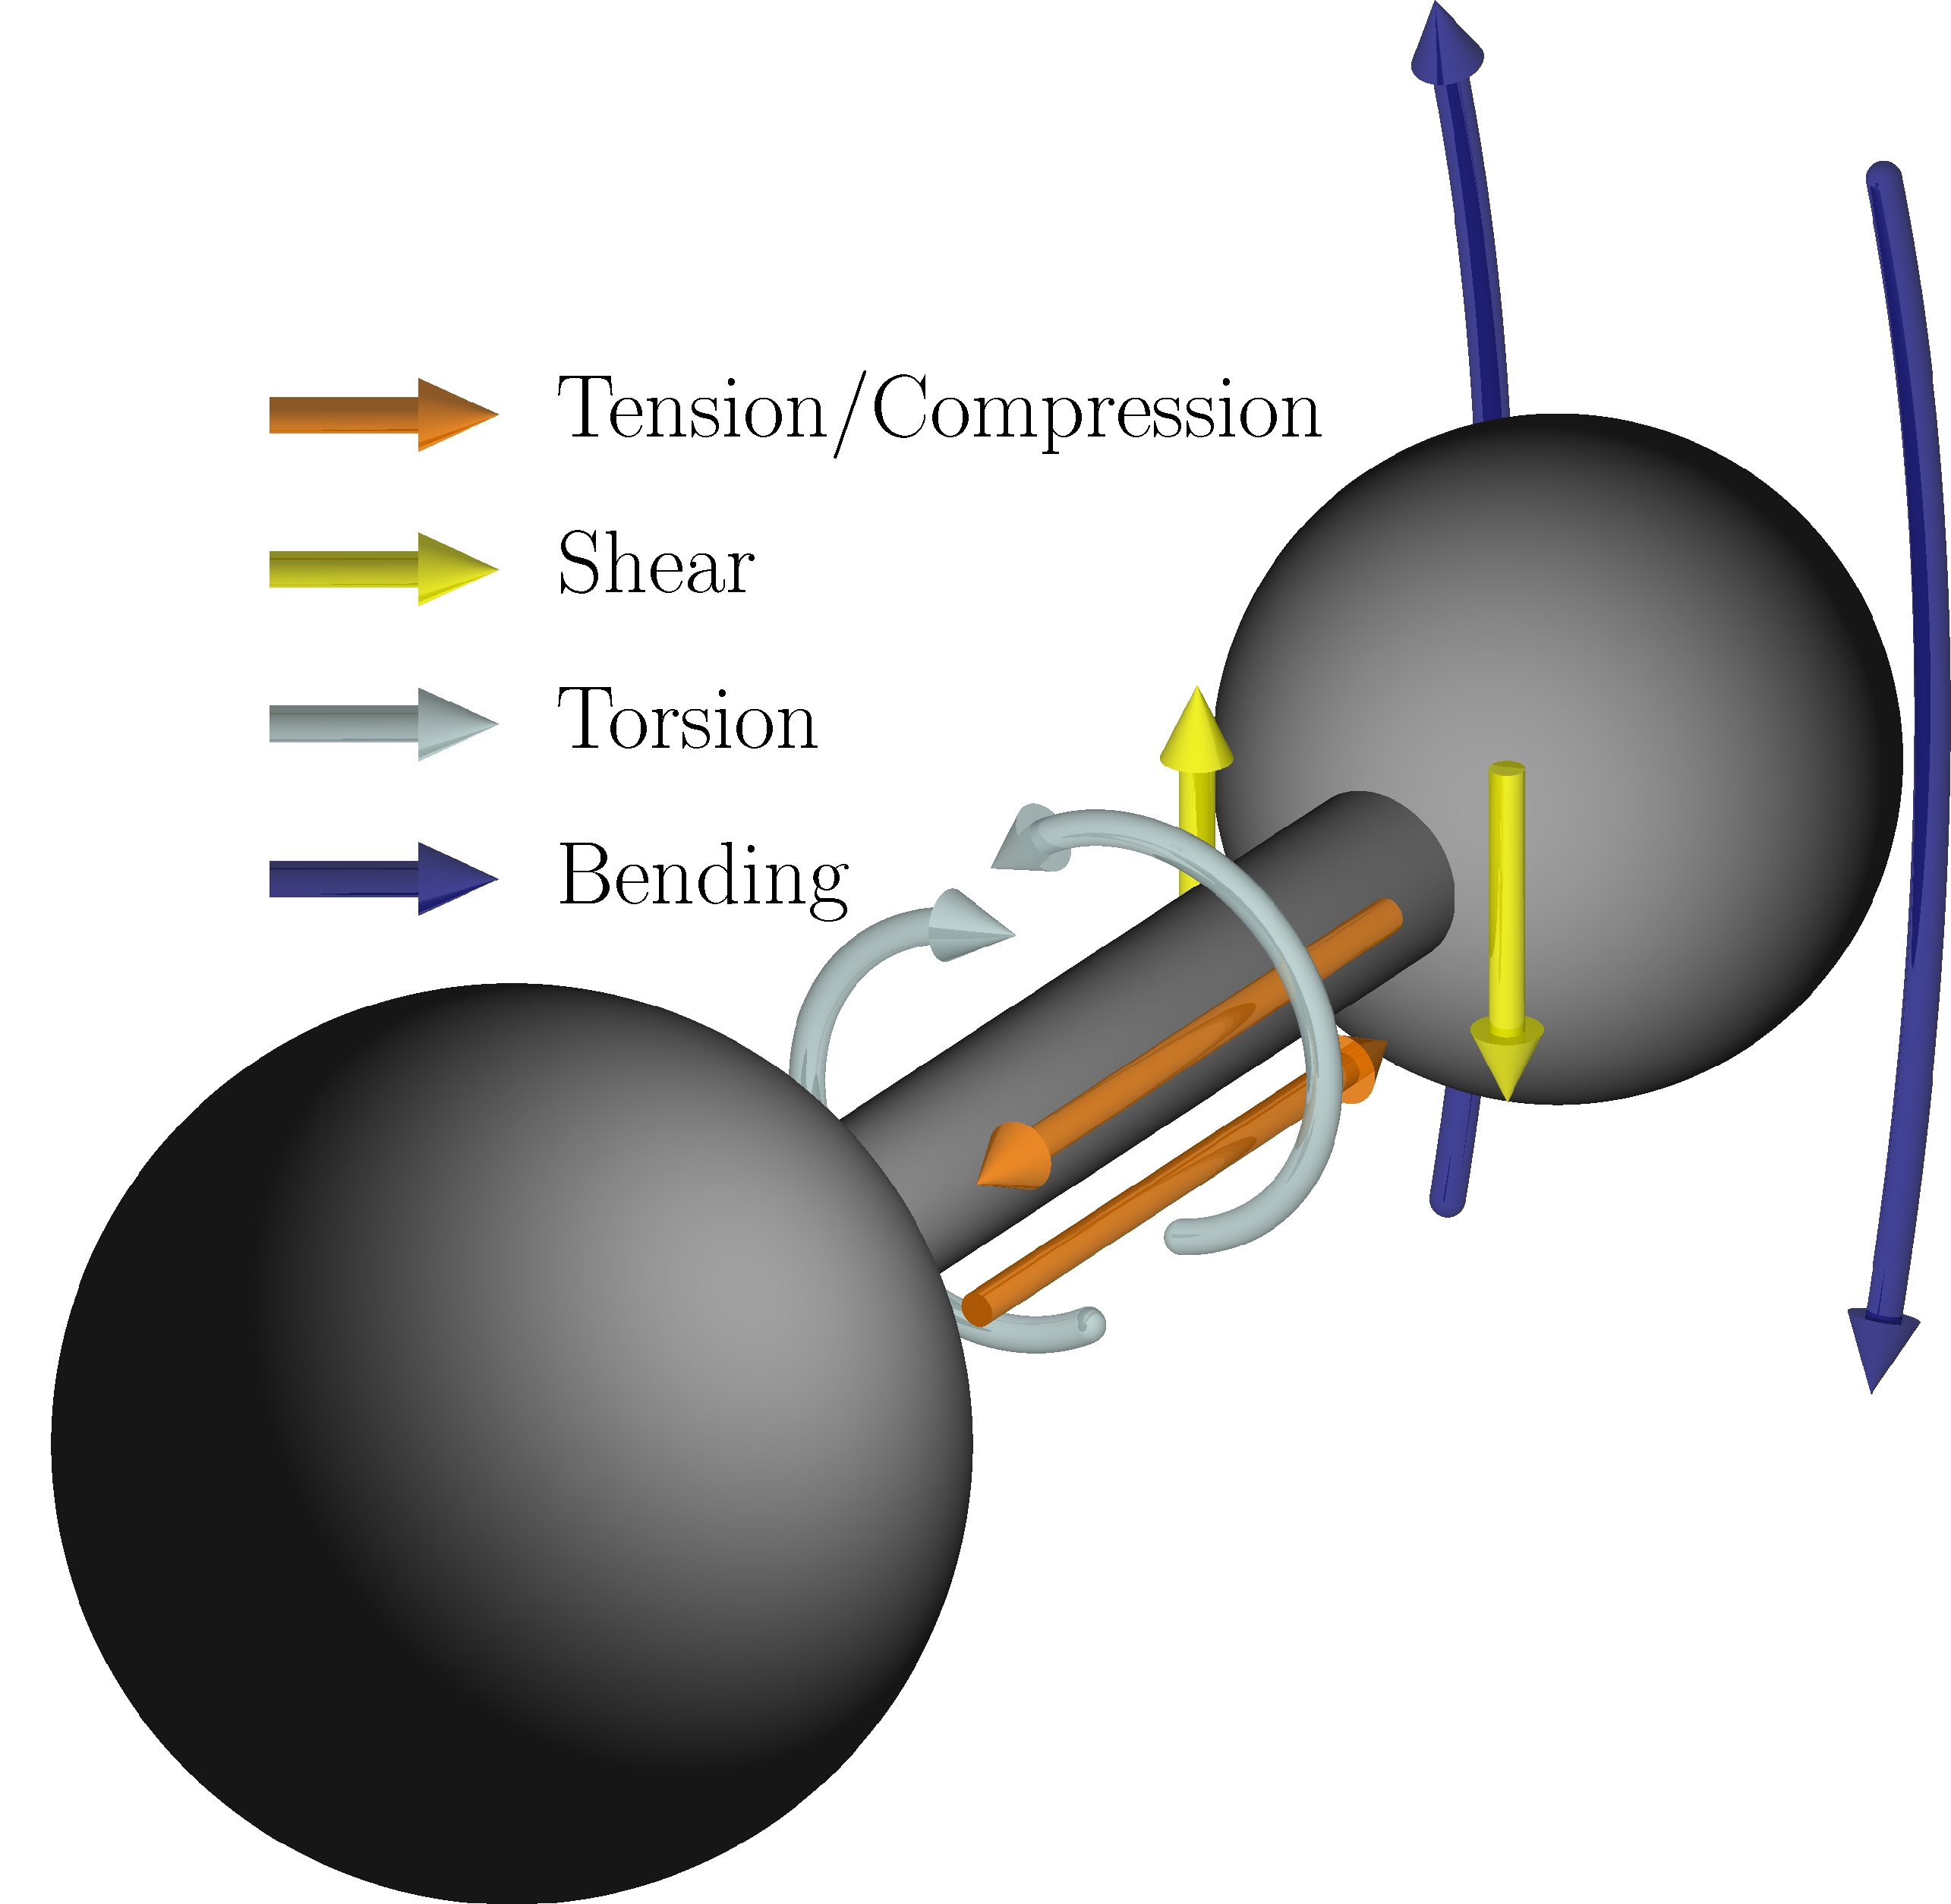
\includegraphics{rotational_bonds.jpg}}
\end{center}
\end{minipage}
\begin{minipage}{3in}
\caption{Diagram illustrating the forces and moments between particles bonded via rotational elastic-brittle bonds} \label{fig:rot_bond_diagram}
\end{minipage}
\end{figure}


There is also a \texttt{FrictionPrms} interaction specifically designed for frictional interactions between unbonded rotational particles. Unlike the non-rotational equivalent, rotational frictional interactions impart a torque to both particles, causing the particles to rotate relative to each other when in frictional contact. 

The following code-fragment defines the microphysical parameters of rotational bonds: 

\begin{verbatim}
#create rotational elastic-brittle bonds between particles:
pp_bonds = sim.createInteractionGroup (
   BrittleBeamPrms(
      name="pp_bonds",
      youngsModulus=100000.0,
      poissonsRatio=0.25,
      cohesion=100.0,
      tanAngle=1.0,
      tag=1
   )
)
\end{verbatim}

\noindent
The \texttt{tag} parameter is used to specify which particle-pairs should be bonded together. The bond tags were assigned by the \texttt{ConnectionFinder} in the previous section. 

%It should be emphasised that the Young's Modulus, Poisson's ratio, cohesion and internal angle of friction (\texttt{tanAngle}) refer to the microphysical properties of individual brittle-elastic beams connecting two particles. Although the macroscopic elastic properties of the bonded particle assembly are strongly related to these parameters, there is typically not a one-to-one correspondence.

%Rotational brittle-elastic bonds require specification of four parameters: two governing elastic properties of bonds and two governing the breaking strength of bonds. 

The physical interpretation of rotational bonds is that two particles are connected to one another with a cylindrical elastic beam whose radius is the mean of the radii of the bonded particles and whose equilibrium length is the sum of the radii of those particles. The elasticity of bonds is determined by a microscopic Young's modulus (\texttt{youngsModulus} parameter) and a microscopic Poisson's ratio (\texttt{poissonsRatio} parameter). It should be emphasised that the macroscopic elastic properties of an assembly of bonded particles does not necessarily match the microscopic elastic properties of the bonds themselves. The topology of the bond network in a particle assembly also influences its macroscopic elastic properties.

In order to simulate brittle failure of samples, bonds require a failure threshold criterion (or breaking strength). In ESyS-Particle, a Mohr-Coulomb failure criterion is employed. A bond will fail (or break) if the shear stress within the bond exceeds its shear strength ($\tau$) given by:

\begin{equation}
\tau = \mathcal{C} + \sigma_N \tan (\phi_f)
\end{equation}

\noindent
where $\mathcal{C}$ is the cohesive strength of the bond for zero normal stress ($\sigma_N$) and $\phi_f$ is the internal angle of friction of the bond. The \texttt{cohesion} and \texttt{tanAngle} parameters respectively define the cohesive strength and friction angle of bonds.

%These breakage forces determine a threshold failure condition that once exceeded, causes the bond to break irreversibly. The threshold failure condition is defined as follows:

%\begin{equation}
%\frac{| F_n |}{F^{brk}_n} + \frac{| F_s |}{F^{brk}_s} + \frac{| F_b |}{F^{brk}_b} + \frac{| F_t |}{F^{brk}_t} > 1 \ \ \ .
%\end{equation}

%\vskip 5mm
%\begin{minipage}{5.75in}
%\emph{\textbf{IMPORTANT:} Since version $2.0$ of ESyS-Particle, the implementation of rotational bonded and frictional interactions has changed slightly to fix a problem with the scaling of elastic properties of models containing particles with differing radii (as is the case in this tutorial). By default, ESyS-Particle now interprets elastic stiffness parameters (e.g. \texttt{normalK} and \texttt{torsionK}) as elastic contact moduli (in stress) units. Internally ESyS-Particle multiplies these constants by the mean radius of two bonded (or touching) particles to compute a per-bond elastic stiffness. Similarly the breaking force parameters are interpreted as yield stresses. ESyS-Particle multiplies the yield stress parameters by the mean cross-sectional area of bonded particles to compute per-bond breaking forces. If you do not wish to apply this scaling of elastic properties, you need to set \texttt{scaling = False} in the specification of \texttt{RotBondPrms} and \texttt{RotFrictionPrms}. If you do not include the \texttt{scaling} parameter when specifying these types of interactions, ESyS-Particle assumes by default that \texttt{scaling = True} and will issue a warning to remind you about the \texttt{scaling} parameter.
%\end{minipage}
%\vskip 5mm

When a bond between two particles breaks, we need to specify the type of unbonded interactions the particles will experience should they come into contact. Since a broken bond represents a fracture surface, it is appropriate to specify frictional interactions between unbonded particles. The following code-fragment implements frictional interactions between unbonded, touching particles:

\begin{verbatim}
#initialise frictional interactions for unbonded particles:
sim.createInteractionGroup (
   FrictionPrms(
      name="friction",
      youngsModulus=100000.0,
      poissonsRatio=0.25,
      dynamicMu=0.4,
      staticMu=0.6
   )
)
\end{verbatim}

\noindent
Rotational frictional interactions are defined by a microscopic Young's modulus (\texttt{youngs\+Mod\+u\+lus}) and Poisson's ratio (\texttt{poissonsRatio}) and two microscopic coefficients of friction. Typically the Young's modulus and Poisson's ratio for \texttt{FrictionPrms} interactions are set equal to their \texttt{BrittleBeamPrms} counterparts. The \texttt{staticMu} coefficient of friction is applied when two particles are in static frictional contact, i.e., prior to the first time the frictional sliding criterion is met. Thereafter the \texttt{dynamicMu} coefficient of friction is applied. By setting $\texttt{dynamicMu} < \texttt{staticMu}$, one can simulate the physical observation that the frictional force required to maintain sliding is less than the force necessary to initiate sliding.

Finally, we must inform the simulation object that any given particle-pair undergoes either bonded interactions or frictional interactions but not both. This is achieved by specifying an \emph{exclusion} between the two interaction groups:

\begin{verbatim}
#create an exclusion between bonded and frictional interactions:
sim.createExclusion (
   interactionName1 = "pp_bonds",
   interactionName2 = "friction"
)
\end{verbatim}

\subsubsection{Implementation of viscous damping}

Uniaxial compression experiments are usually conducted in the so-called quasi-static regime. In other words, external loads are applied slowly compared with the compressional wavespeed of the sample. Any acoustic emissions generated during fracturing dissipate rapidly compared with the duration of the experiment. To simulate these conditions, we must also incorporate two body forces designed to attenuate translational and rotational oscillations. In previous examples we encountered the \texttt{LinDamping} body force. In the uniaxial compression simulations we will use both \texttt{LinDamping} and \texttt{RotDamping}, the later being designed to attenuate rotational oscillations. The two damping forces are implemented thus:

\begin{verbatim}
#add translational viscous damping:
sim.createInteractionGroup (
   LinDampingPrms(
      name="damping1",
      viscosity=0.002,
      maxIterations=50
   )
)

#add rotational viscous damping:
sim.createInteractionGroup (
   RotDampingPrms(
      name="damping2",
      viscosity=0.002,
      maxIterations=50
   )
)
\end{verbatim}

\noindent
The viscosity coefficients are chosen to be small so that damping has little effect on the elastic response of the simulated rock sample but it is sufficient to attenuate unwanted oscillations. 

\subsubsection{Implementation of movable walls: the \texttt{WallLoader} \texttt{Runnable}}

Only one component remains to be added to the uniaxial compression simulation: a method to move the two walls at constant speed. There are a couple of ways this may be implemented: either  as a subroutine that is called each timestep of the simulation or as a reusable \texttt{Runnable} module. We previously encountered \texttt{Runnables} in the first tutorial. The use of a \texttt{Runnable} is considered superior as the module can be re-used in subsequent simulations whenever movable walls are required. 

There are two steps involved in implementing and using a \texttt{Runnable}:
\begin{enumerate}
\item Write a script containing the implementation of the \texttt{Runnable}, and
\item Add the runnable into the simulation container.
\end{enumerate}

\noindent
The following code (entitled \texttt{WallLoader.py} in Appendix~\ref{code}) implements a \texttt{Runnable} to move a given wall with a specified velocity. To achieve this, the \texttt{Runnable} must be passed a reference to the simulation object, a wall name, a velocity and two additional parameters: \texttt{startTime} and \texttt{rampTime}. Experience has shown that it is best to gradually increase the wall speed from zero to the desired value over a few hundred timesteps. The \texttt{rampTime} parameter specifies the number of timesteps during which the wall accelerates. The velocity of the wall increases linearly over that number of timesteps. The other parameter (\texttt{startTime}) allows the user to commence moving the wall after a specified number of timesteps. 

The \texttt{WallLoader} \texttt{Runnable} has two subroutines:
\begin{itemize} 
\item \texttt{\_\_init\_\_()} to initialise the \texttt{Runnable} and store parameter values, and
\item \texttt{run()} which moves the wall and is called once each timestep of the simulation.
\end{itemize} 

\noindent
The implementation of the \texttt{WallLoader} \texttt{Runnable} is as follows:

\begin{verbatim}
#import the appropriate ESyS-Particle modules:
from esys.lsm import *
from esys.lsm.util import *

class WallLoaderRunnable (Runnable):
   def __init__ (self, 
                 LsmMpi=None, 
                 wallName=None, 
                 vPlate=Vec3(0,0,0), 
                 startTime=0, 
                 rampTime = 200):
      """
      Subroutine to initialise the Runnable and store parameter values.
      """
      Runnable.__init__(self)
      self.sim = LsmMpi
      self.wallName = wallName
      self.Vplate = vPlate
      self.dt = self.sim.getTimeStepSize()
      self.rampTime = rampTime
      self.startTime = startTime
      self.Nt = 0

   def run (self):
      """
      Subroutine to move the specified wall. After self.startTime 
      timesteps, the speed of the wall increases linearly over 
      self.rampTime timesteps until the desired wall speed is achieved. 
      Thereafter the wall is moved at that speed.
      """
      if (self.Nt >= self.startTime):

         #compute the slowdown factor if still accelerating the wall:
         if (self.Nt < (self.startTime + self.rampTime)):
            f = float(self.Nt - self.startTime) / float(self.rampTime)
         else:
            f = 1.0

         #compute the amount by which to move the wall this timestep:
         Dplate = Vec3(
            f*self.Vplate[0]*self.dt, 
            f*self.Vplate[1]*self.dt, 
            f*self.Vplate[2]*self.dt
         )
         #instruct the simulation to move the wall:
         self.sim.moveWallBy (self.wallName, Dplate)

      #count the number of timesteps completed thus far:
      self.Nt += 1
\end{verbatim}

\noindent
Copy the code above into a text file called \texttt{WallLoader.py} and save it in the same directory as the file containing the code for the uniaxial compression simulation (called \texttt{rot\_compress.py} in Appendix~\ref{code}).

To use this \texttt{Runnable} in the uniaxial compression simulation, we must do two things: 
\begin{enumerate}
\item import the Runnable at the start of the script like so:
\begin{verbatim}
from WallLoader import WallLoaderRunnable
\end{verbatim}
\item add a \texttt{WallLoaderRunnable} for each of the two piston walls:
\begin{verbatim}
#add a wall loader to move the top wall:
wall_loader1 = WallLoaderRunnable(
   LsmMpi = sim,
   wallName = "top_wall",
   vPlate = Vec3 (0.0, -0.125, 0.0),
   startTime = 0,
   rampTime = 50000
)
sim.addPreTimeStepRunnable (wall_loader1)

#add a wall loader to move the bottom wall:
wall_loader2 = WallLoaderRunnable(
   LsmMpi = sim,
   wallName = "bottom_wall",
   vPlate = Vec3 (0.0, 0.125, 0.0),
   startTime = 0,
   rampTime = 50000
)
sim.addPreTimeStepRunnable (wall_loader2)
\end{verbatim}
\end{enumerate}

\noindent
Notice that the sign of the wall velocity (\texttt{vPlate}) is opposite for the two walls. The top wall will move downwards and the bottom wall upwards, both at a speed of $0.125$~m/s. Although this rate is significantly higher than that typically used in laboratory uniaxial compression experiments, it is sufficiently small to maintain quasi-static conditions in the simulations. The piston speeds are approximately $20000 \times$ lower than the compressional wavespeed of the simulated rock sample. The initial acceleration of the walls from zero to the desired speed (during the first $50000$ timesteps) also helps ensure the sample is loaded quasi-statically. 

Technically the simulation object now contains all of the components needed for a uniaxial compression simulation.  The only remaining item is to instruct the simulation to execute all timesteps. This is achieved with the following command:

\begin{verbatim}
#execute the simulation:
sim.run()
\end{verbatim}

\noindent
If you have been following the previous tutorials, you may notice that we have not specified how data should be output during the simulation. This is covered in detail in the next section, where we discuss the use of \texttt{FieldSavers} to store only the data of specific interest during uniaxial compression simulations.

\subsection{Measurement of macroscopic elastic properties}

One of the primary reasons for conducting uniaxial compression simulations is to measure the Young's modulus and Unconfined Compressive Strength (UCS) of the rock sample. Both of these macroscopic properties can be obtained from a stress--strain curve, as illustrated in Figure~\ref{fig:stress_strain_diag}. Young's modulus is defined as the slope of the linear section of the stress--strain curve, whilst the UCS is the peak value of the stress. In order to measure these quantities in a simulation, we must construct the stress--strain curve for the simulation. 

\begin{figure}
\begin{center}
\resizebox{5in}{!}{
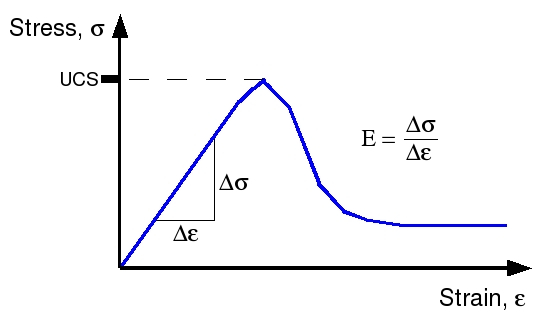
\includegraphics{stress_strain_diagram.jpg}}
\end{center}
\caption[Diagram illustrating a typical stress-strain curve \& how to measure Young's modulus ($E$) \& the unconfined compressive strength (UCS) from such a curve]{Diagram illustrating a typical stress-strain curve and how to measure Young's modulus ($E$) and the unconfined compressive strength (UCS) from such a curve} \label{fig:stress_strain_diag}
\end{figure}

Suppose the net restoring forces (at time $t$) that particles apply to the top and bottom walls are $\vec{F}^{(t)} (t)$ and $\vec{F}^{(b)} (t)$ respectively, and the unit normal vector of the walls is $\hat{n}^{(t/b)}$. Then the stress exerted on the walls by the particle assembly is:

\begin{equation}
\sigma_{YY} (t) = \frac{\vec{F}^{(t)} . \hat{n}^{(t)} + \vec{F}^{(b)} . \hat{n}^{(b)}}{2 A_c} \ \ \ , \label{eq:stress}
\end{equation}

\noindent
where $A_c$ is contact area between a wall and the particle assembly. Since the peak stress is reached for relatively small axial strain (only a few \% usually), the contact area can be approximated by the undeformed area of base of the particle assembly (in our example, that would be $10 \mathrm{m} \times 10 \mathrm{m} = 100 \mathrm{m}^2$). 

Computing the total strain is also relatively straightforward. Let $\vec{X}^{(t)} (t)$ and $\vec{X}^{(b)} (t)$ be the positions of the top and bottom walls at time $t$. The strain $\varepsilon_{YY} (t)$ is given by:

\begin{eqnarray} 
\varepsilon_{YY} (t) & = & \frac{\left[ \left( \vec{X}^{(t)} (0) - \vec{X}^{(b)} (0) \right) - \left( \vec{X}^{(t)} (t) - \vec{X}^{(b)} (t) \right) \right] . \hat{y}}{\left[ \left( \vec{X}^{(t)} (0) - \vec{X}^{(b)} (0) \right) \right] . \hat{y}} \\
 & = & 1 - \frac{\left[ \vec{X}^{(t)} (t) - \vec{X}^{(b)} (t) \right] . \hat{y}}{\left[ \vec{X}^{(t)} (0) - \vec{X}^{(b)} (0) \right] . \hat{y}} \label{eq:strain}
\end{eqnarray} 

\noindent
where $\hat{y}$ is the unit vector in the direction normal to the bottom wall.

From the two formulae above, it is evident that to compute the stress--strain curve, we need to record the net force acting on each wall and the position of each wall at each timestep of the simulation. The next section describes how to use \texttt{FieldSavers} to store the forces and positions of walls. In the following section, we will examine how to read the output files and construct the stress--strain curve for a simulation.

\subsubsection{Storing wall positions and forces}

ESyS-Particle includes a group of modules called \texttt{FieldSavers} designed to store specific simulation data to disk. \texttt{FieldSavers} are closely related to the \texttt{CheckPointer} encountered in the first tutorial, the main difference being that \texttt{FieldSavers} store only specific data rather than all of the state variables of the particles. \texttt{FieldSavers} can also be used to store data on particles (such as position or kinetic energy), interactions (such as potential energy and the number of broken bonds), and walls (such as the position of a wall and the net force acting on the wall). 

As discussed in the previous section, we need to store the wall forces and positions in order to construct the stress--strain curve for our uniaxial compression simulations. The following code-fragment initialises a \texttt{FieldSaver} to store wall positions:

\begin{verbatim} 
#create a FieldSaver to wall positions:
posn_saver = WallVectorFieldSaverPrms(
   wallName=["bottom_wall", "top_wall"],
   fieldName="Position",
   fileName="out_Position.dat",
   fileFormat="RAW_SERIES",
   beginTimeStep=0,
   endTimeStep=250000,
   timeStepIncr=10
)
sim.createFieldSaver(posn_saver)
\end{verbatim} 

\noindent
This code-fragment should be inserted before \texttt{sim.run()} is called.  \texttt{WallVec\+torFieldSav\+erPrms} takes a number of parameters. These are:

\begin{itemize}
\item \texttt{wallName} -- a list of the names of walls whose position you wish to save
\item \texttt{fieldName} -- the data field to store (in this case ``Position'')
\item \texttt{fileName} -- the name of the text file in which to store the data
\item \texttt{fileFormat} -- the output format (\texttt{RAW\_SERIES} creates an ASCII text file)
\item \texttt{beginTimeStep} -- the timestep number to commence storing data
\item \texttt{endTimeStep} -- the timestep number to conclude storing data
\item \texttt{timeStepIncr} -- the number of timesteps to wait between storing a datum
\end{itemize}

\noindent
Storing wall forces is very similar -- one need only specify a \texttt{fieldName} of \texttt{Force} and change the \texttt{fileName}. The following code fragment will initialise a \texttt{FieldSaver} to store wall forces:

\begin{verbatim}
#create a FieldSaver to wall forces:
force_saver = WallVectorFieldSaverPrms(
   wallName=["bottom_wall", "top_wall"],
   fieldName="Force",
   fileName="out_Force.dat",
   fileFormat="RAW_SERIES",
   beginTimeStep=0,
   endTimeStep=250000,
   timeStepIncr=10
)
sim.createFieldSaver(force_saver)
\end{verbatim}

\subsubsection[Measurement of Young's modulus \& unconfined compressive strength]{Measurement of Young's modulus and unconfined compressive strength}

Once you have written all the code-fragments above into a text file (called \texttt{rot\_\+com\+press.py}) and created a \texttt{WallLoader.py} file containing the implementation of the \texttt{Wall\+Load\+er} \texttt{Runnable}, execute a simulation by typing the following at the command prompt:

\begin{verbatim}
$ mpirun -np 2 `which esysparticle` rot_compress.py
\end{verbatim}

\noindent
The simulation may take some time so feel free to go grab a coffee while you wait! 

When the simulation is completed, two text files should have been written into the current working directory, \texttt{out\_Position.dat} and \texttt{out\_Force.dat}. If you examine one of these files with a text editor, the first few lines should look something like the following:

\begin{verbatim}
0 1.125e-10 0  0 20 0  
0 4.75e-10 0  0 20 0  
0 1.0875e-09 0  0 20 0  
0 1.95e-09 0  0 20 0  
0 3.0625e-09 0  0 20 0  
0 4.425e-09 0  0 20 0  
0 6.0375e-09 0  0 20 0  
0 7.9e-09 0  0 20 0  
0 1.00125e-08 0  0 20 0  
0 1.2375e-08 0  0 20 0
\end{verbatim}

\noindent
The file is formatted so that, for any given timestep, the vector position (or force) of each wall is listed one after the other on the same line. Hence, the first 3 columns are the X-, Y- and Z-components of the position (or force) of the bottom wall and the following 3 columns are those of the top wall. 

The following python script will read both files and output stress and strain at each timestep in a format suitable for plotting using \texttt{gnuplot} or another XY plotting package. The formulae used to compute stress and strain are Equations~\ref{eq:stress} and \ref{eq:strain}. Figure~\ref{fig:UCS_stress_strain} shows the result for a typical uniaxial compression simulation.

\begin{verbatim}
from math import *

posnfile = open("out_Position.dat","r")
posn = posnfile.readlines()
posnfile.close()

forcefile = open("out_Force.dat","r")
force = forcefile.readlines()
forcefile.close()

for i in range (len(posn)):
   Y_bottom = float(posn[i].split()[1])
   Y_top = float(posn[i].split()[4])
   F_bottom = float(force[i].split()[1])
   F_top = float(force[i].split()[4])

   stress = (F_bottom - F_top)/100.0
   strain = 1.0 - (Y_top - Y_bottom)/20.0
   print strain,stress
\end{verbatim}

\noindent
To execute this script, write it to a text file called \texttt{make\_stress\_strain.py}, save it to the same directory where you ran the uniaxial compression simulation, then type the following at the command prompt: 

\begin{verbatim}
$ python make_stress_strain.py > stress_strain.dat
\end{verbatim}

\noindent
A new text file (called \texttt{stress\_strain.dat}) will be created, the first column of which will be strain and the second will be stress. 

Now that we have a stress-strain curve for the uniaxial compression simulation, it is a simple matter to measure the slope of the linear section to estimate Young's modulus and to measure the peak stress -- an estimate for the unconfined compressive strength. You might like to write your own script to compute Young's modulus and UCS directly from \texttt{stress\_strain.dat} or modify the script above.

In the next section we will examine three more useful \texttt{FieldSavers} for uniaxial compression simulations, namely the total kinetic energy of the particles, the total strain energy stored in bonds and the number of broken bonds. These three fields provide information on the internal deformation of the simulated rock sample, quantities not usually directly amenable to measurement in laboratory experiments.

\begin{figure}
\begin{center}
\resizebox{5in}{!}{
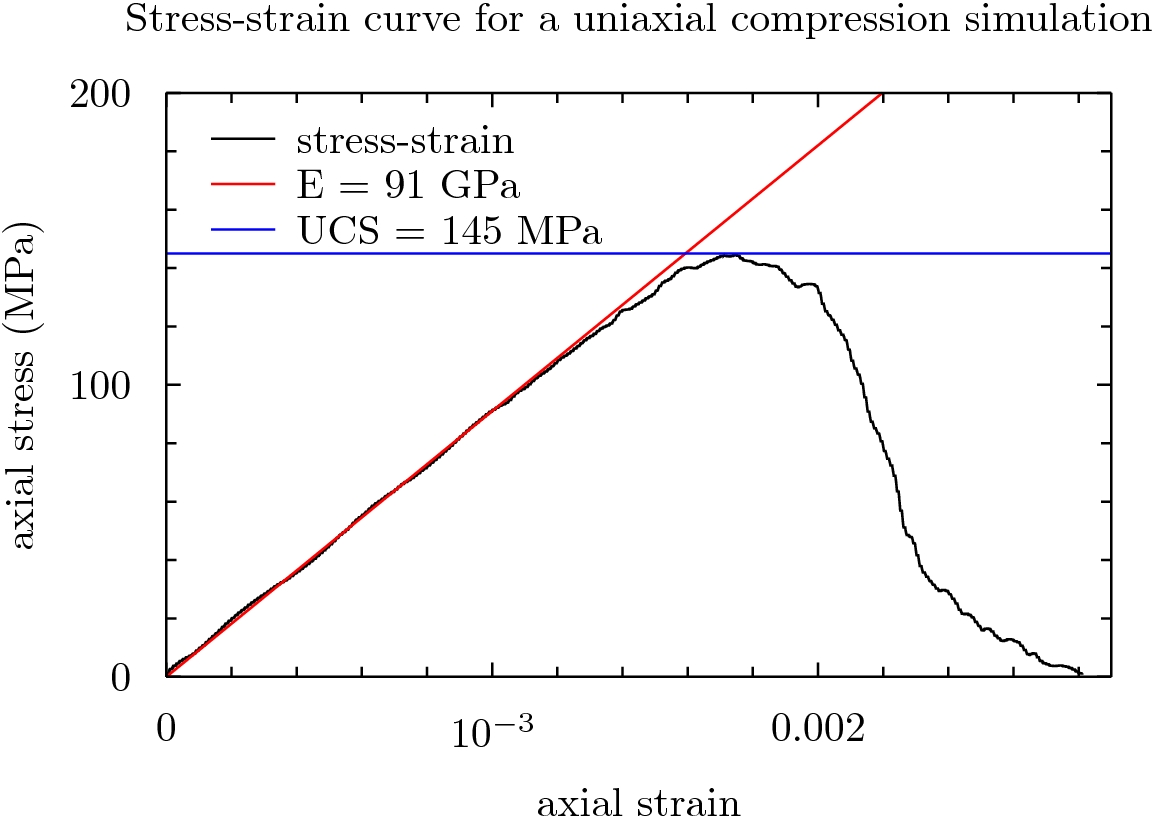
\includegraphics{UCS_stress_strain.jpg}}
\end{center}
\caption{Stress-Strain curve obtained from a uniaxial compression simulation (from \texttt{rot\_compress.py})} \label{fig:UCS_stress_strain}
\end{figure}


\subsubsection{Storing information on particles and bonds: kinetic energy, potential energy and number of bonds}

In the previous section we examined how to output wall forces and positions using \texttt{FieldSavers}. Both these data fields are examples of \emph{measurable quantities}, i.e., quantities that can be directly measured in equivalent laboratory experiments. Comparison of measurable quantities from simulations and experiments is a useful technique for validating and calibrating Discrete Element models. However, the primary advantage of computer simulations in scientific research is the ability to examine internal dynamics that are typically not amenable to direct observation in the laboratory or field. In this section we examine three quantities that provide insight on the internal deformation within rock samples subjected to uniaxial compressive loads. 

The first quantity is the total kinetic energy of the particle assembly. The total kinetic energy is simply the sum of the kinetic energy of each particle, i.e., $E_k = \sum_i \frac{1}{2} m_i v_i^2$. It is frequently useful to measure the total kinetic energy in simulations, particularly if one suspects a simulation is numerically unstable. An unbounded growth in the total kinetic energy over time is a good indication that a simulation is not working correctly. The following code-fragment initialises a \texttt{ParticleScalarFieldSaver} to store the total kinetic energy each timestep:

\begin{verbatim}
#create a FieldSaver to store the total kinetic energy of the particles:
sim.createFieldSaver (
   ParticleScalarFieldSaverPrms(
      fieldName="e_kin",
      fileName="ekin.dat",
      fileFormat="SUM",
      beginTimeStep=0,
      endTimeStep=250000,
      timeStepIncr=1
   )
)
\end{verbatim}

\noindent
Most of the \texttt{FieldSaver} parameters should now be familiar.  A new \texttt{fileFormat} called \texttt{SUM} is used here. This file format stores the sum of the kinetic energy of each particle. The output format is an ASCII text file with the total kinetic energy written once per timestep.  A number of other fields may also be output using \texttt{ParticleScalarFieldSavers} or \texttt{ParticleVectorFieldSavers}. A list of valid \texttt{fieldNames} for various types of \texttt{FieldSav\+ers} is provided in Appendix \ref{tables}.  Other helpful information can be found on this \link{ESyS-Particle wiki documentation page}{https://wiki.geocomp.uq.edu.au/index.php/Documentation_and_Presentations}. 

The second quantity is the total strain energy stored within bonds connecting particles. The total strain energy is simply the sum of the potential energies of the rotational bonds connecting each particle-pair. The following code-fragment initialises an \texttt{InteractionScalarFieldSaver} to store the total strain energy each timestep:

\begin{verbatim}
#create a FieldSaver to store potential energy stored in bonds:
sim.createFieldSaver (
   InteractionScalarFieldSaverPrms(
      interactionName="pp_bonds",
      fieldName="potential_energy",
      fileName="epot.dat",
      fileFormat="SUM",
      beginTimeStep=0,
      endTimeStep=250000,
      timeStepIncr=1
   )
)
\end{verbatim}

\noindent
Notice that instead of providing a list of wall names, we now provide the name of the Interaction Group, whose data we wish to store (in this case our \texttt{pp\_bonds} interaction group defining rotational bonds between particles). Once again we specify a \texttt{SUM fileFormat} so that the total potential energy is output to an ASCII text file once per timestep.

Another extremely useful quantity to monitor in elastic-brittle simulations is the number of broken bonds, as this is a measure of the amount of damage the rock sample has suffered due to the external load. Another \texttt{InteractionScalarFieldSaver} is used to output the total number of bonds each timestep. The relevant code-fragment is as follows:

\begin{verbatim}
#create a FieldSaver to store number of bonds:
sim.createFieldSaver (
   InteractionScalarFieldSaverPrms(
      interactionName="pp_bonds",
      fieldName="count",
      fileName="nbonds.dat",
      fileFormat="SUM",
      beginTimeStep=0,
      endTimeStep=250000,
      timeStepIncr=1
   )
)
\end{verbatim}

\noindent
The main difference here is the choice of \texttt{fieldName} -- \texttt{count} instead of \texttt{potential\_energy}. Note that this \texttt{FieldSaver} will output the total number of remaining bonds. If you wish to know how many bonds have broken you need to subtract the total number of remaining bonds from the initial number of bonds. 

\begin{figure}
\begin{center}
\resizebox{5in}{!}{
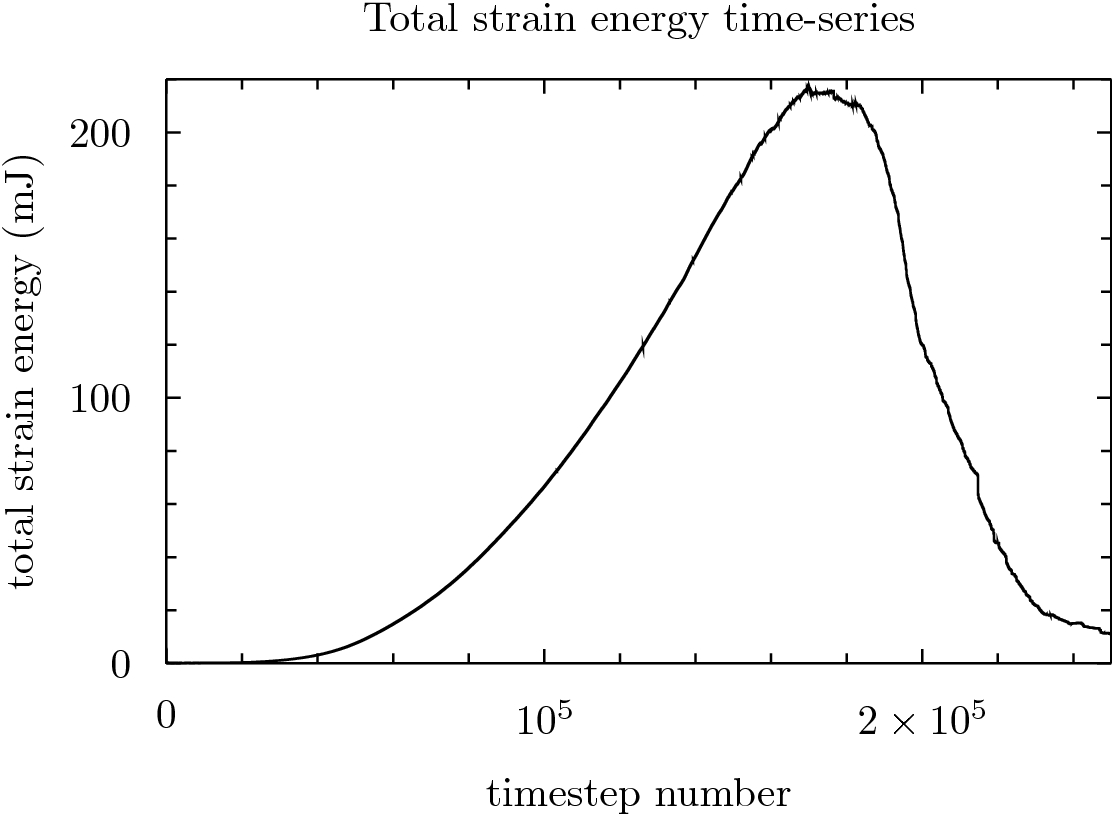
\includegraphics{UCS_epot.jpg}}
\end{center}
\caption{Time-series of total strain energy stored in bonds during a uniaxial compression simulation (from \texttt{rot\_compress.py})} \label{fig:UCS_PE}
\end{figure}

\begin{figure}
\begin{center}
\resizebox{5in}{!}{
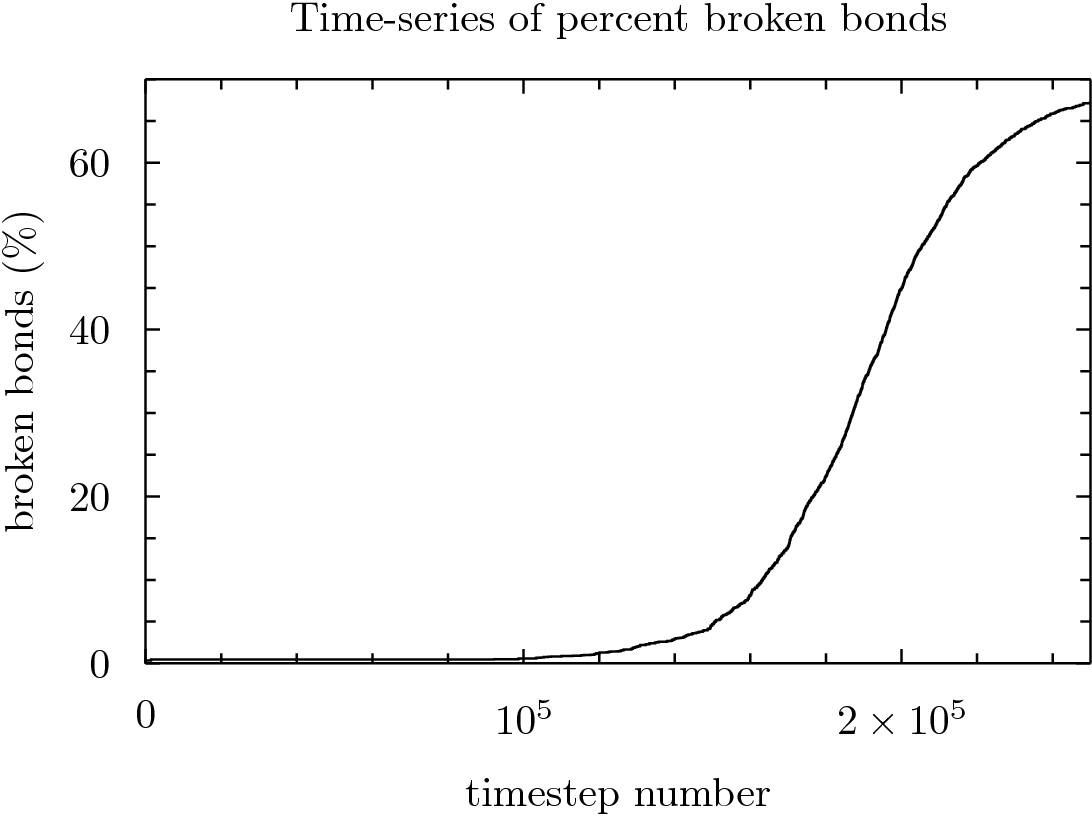
\includegraphics{UCS_nbonds.jpg}}
\end{center}
\caption{Time-series of percentage of bonds broken during a uniaxial compression simulation (from \texttt{rot\_compress.py})} \label{fig:UCS_nbroke}
\end{figure}

\begin{figure}
\begin{center}
\resizebox{5in}{!}{
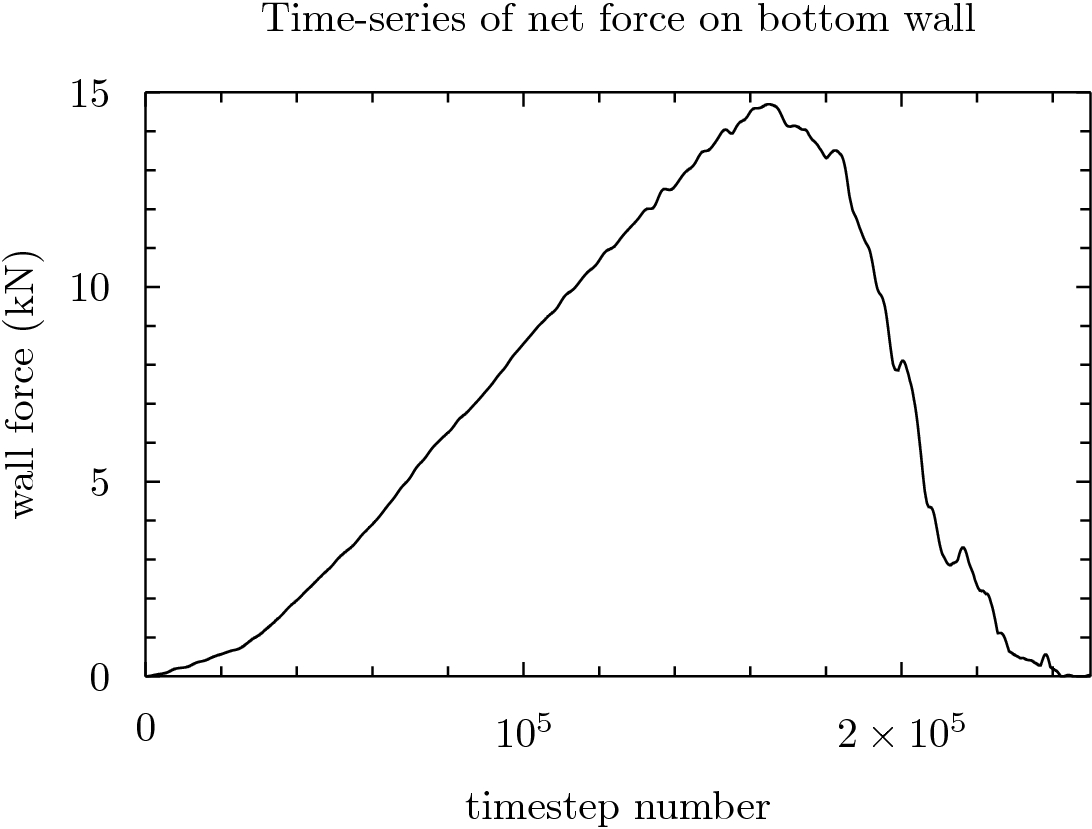
\includegraphics{UCS_force.jpg}}
\end{center}
\caption{Time-series of net wall force during a uniaxial compression simulation (from \texttt{rot\_compress.py})} \label{fig:UCS_force}
\end{figure}

Time-series of the total strain energy and the number of broken bonds are shown in Figures~\ref{fig:UCS_PE} and \ref{fig:UCS_nbroke} along with the wall force time-series (Figure~\ref{fig:UCS_force}) for comparison. The total strain energy time-series closely resembles the stress--strain curve, suggesting that total internal strain energy is proportional to macroscopic stress. This is not that unexpected given that it is the energy stored in bonds that imparts a force on the piston walls. The time-series of broken bonds is more interesting. Firstly, it is apparent that a significant fraction of bonds break before the peak stress is reached. In other words, the sample undergoes significant irreversible internal damage prior to reaching the unconfined compressive strength. The second interesting observation is that the total number of broken bonds after the peak stress is reached is only approximately $30\%$ of the initial number of bonds. The sample remains largely intact even post-peak. This is exactly what 
one would expect in laboratory uniaxial compression experiments as well. These experiments do not entirely annihilate rocks to atoms, but rather fragment the rock samples into a large number of smaller fragments. In a later tutorial, we will discuss how to post-process \texttt{CheckPointer} output files to measure, amongst other things, the sizes and number of fragments produced during our uniaxial compression simulation.

%\subsubsection{Dimensional analysis and rescaling of simulation results}

%\emph{\textbf{TO DO}}

%\subsection{Triaxial compression simulations}

%\subsubsection{Implementation of servo walls}

%\subsubsection{Measurement of Poisson's ratio}

\subsection*{What's Next?}

In this tutorial we introduced three useful features in ESyS-Particle simulations: the ability to move walls via a \texttt{Runnable} to implement external loading of models, new types of particle-pair interactions for models involving rotational particles, and some FieldSavers, providing another mechanism for outputing specific data about particles, walls and interactions during the course of a simulation. We also discussed some of the issues related to calibration of model parameters in DEM simulations. By this stage we have covered most of the basic features of ESyS-Particle simulations, so you are ready to start designing and executing your own simulations. 

In the following tutorial we will encounter some post-processing tools provided with ESyS-Particle. These tools are designed for post-simulation analysis of data stored in \texttt{CheckPointer} output files to permit visualisation and analysis of data that is not easily computed during simulations. We will demonstrate how to convert \texttt{CheckPoint} files into a format suitable for interactive visualisation using popular third-party software such as ParaView and VisIt. We will also see how to visualise the locations of broken bonds and also the shapes of fragments produced during uniaxial compression simulations. 

%In the following tutorials we will start to discuss some of the more advanced features of ESyS-Particle. These include the use of a external helper module called \texttt{LSMGenGeo} that provides the capacity to create particle models of siginificantly greater geometrical complexity than the basic tools covered already (such as \texttt{CubicBlock} and \texttt{RandomBoxPacker}).  We will also introduce some post-processing tools provided with ESyS-Particle designed for post-simulation analysis of data stored in checkpoint files. These tools include a conversion tool to permit interactive visualisation of ESyS-Particle checkpoint files using third-party software such as \link{ParaView}{http://www.paraview.org} and \link{VisIt}{https://wci.llnl.gov/codes/visit/}. 

\newpage
\section{Post-processing and data visualisation}
\label{sec:postprocessing}
ESyS-Particle is primarily designed as a high-performance parallel DEM simulation engine. The Python API makes designing and executing different simulations relatively simple and straightforward, however the data output mechanisms (\texttt{FieldSavers} and \texttt{CheckPointers}) are relatively basic. For most applications, post-processing of simulation output files will be necessary to obtain useful results. ESyS-Particle is packaged with a few tools designed to aid in the post-processing of simulation data to obtain particular results or convert the output into formats that can be visualised using freely available third-party visualisation tools (such as \link{ParaView}{http://www.paraview.org} and \link{VisIt}{https://wci.llnl.gov/codes/visit/}). 

In this tutorial, we will discuss some of these post-processing tools and how to use them for more advanced visualisation of simulation results. By way of motivation we will use the uniaxial compression simulation (\texttt{rot\_compress.py}) discussed in the previous tutorial. By adding a \texttt{CheckPointer} to our simulation and post-processing the checkpoint files, we will be able to:
\begin{itemize}
\item interactively visualise a variety of simulation data, 
\item calculate the size and shape of rock fragments generated, and 
\item visualise the locations of fractures formed during the compression test.
\end{itemize}

We first encountered the \texttt{CheckPointer} in Chapter~3. \texttt{CheckPointers} provide a convenient way to output data from ESyS-Particle simulations. In combination with the post-processing tools described below (amongst others), quite advanced visualisation and analysis of simulation data may be achieved. To begin, add a \texttt{CheckPointer} to the \texttt{rot\_compress.py} script (just before the \texttt{sim.run()} subroutine call), then re-run the simulation:

\begin{verbatim}
sim.createCheckPointer (
   CheckPointPrms (
      fileNamePrefix = "snapshot",
      beginTimeStep = 0,
      endTimeStep = 250000,
      timeStepIncr = 1000
   )
)
\end{verbatim}

\noindent 
A series of \texttt{CheckPoint} files will now have been written to the working directory, each beginning with the prefix \texttt{snapshot}. These checkpoint files provide the input to a number of post-processing tools packed with ESyS-Particle. In this chapter, we will encounter three of these post-processing tools, namely:

\begin{enumerate}
   \item \texttt{dump2vtk}: a tool to convert \texttt{CheckPoint} files into a format suitable for interactive visualisation,
   \item \texttt{grainextract}: a tool that identifies \emph{clusters} of particles bonded together, and
   \item \texttt{fracextract}: a tool for visualising the location of broken bonds in brittle failure simulations.
\end{enumerate}

\subsection{Interactive visualisation of simulation data}

Perhaps the most versatile of ESyS-Particle's post-processing tools is \texttt{dump2vtk}. This tool will convert a sequence of \texttt{CheckPoint} files (also known as \emph{dump} files) into VTK unstructured mesh files. VTK (short for \link{Visualisation Tool Kit}{http://www.vtk.org}) is a popular library for three-dimensional post-processing and visualisation of scientific datasets. Although designed primarily for advanced visualisation and analysis of mesh-based datasets (e.g. from finite difference or finite element software), VTK has quite some utility for post-analysis of DEM simulation data also. Third-party visualisation software (such as \link{ParaView}{http://www.paraview.org} and \link{VisIt}{https://wci.llnl.gov/codes/visit/}) provide interactive 3D visualisation capabilities that make these packages (in combination with \texttt{dump2vtk}) a powerful addition to an ESyS-Particle modeller's arsenal.  

\begin{figure}
\resizebox{\textwidth}{!}{
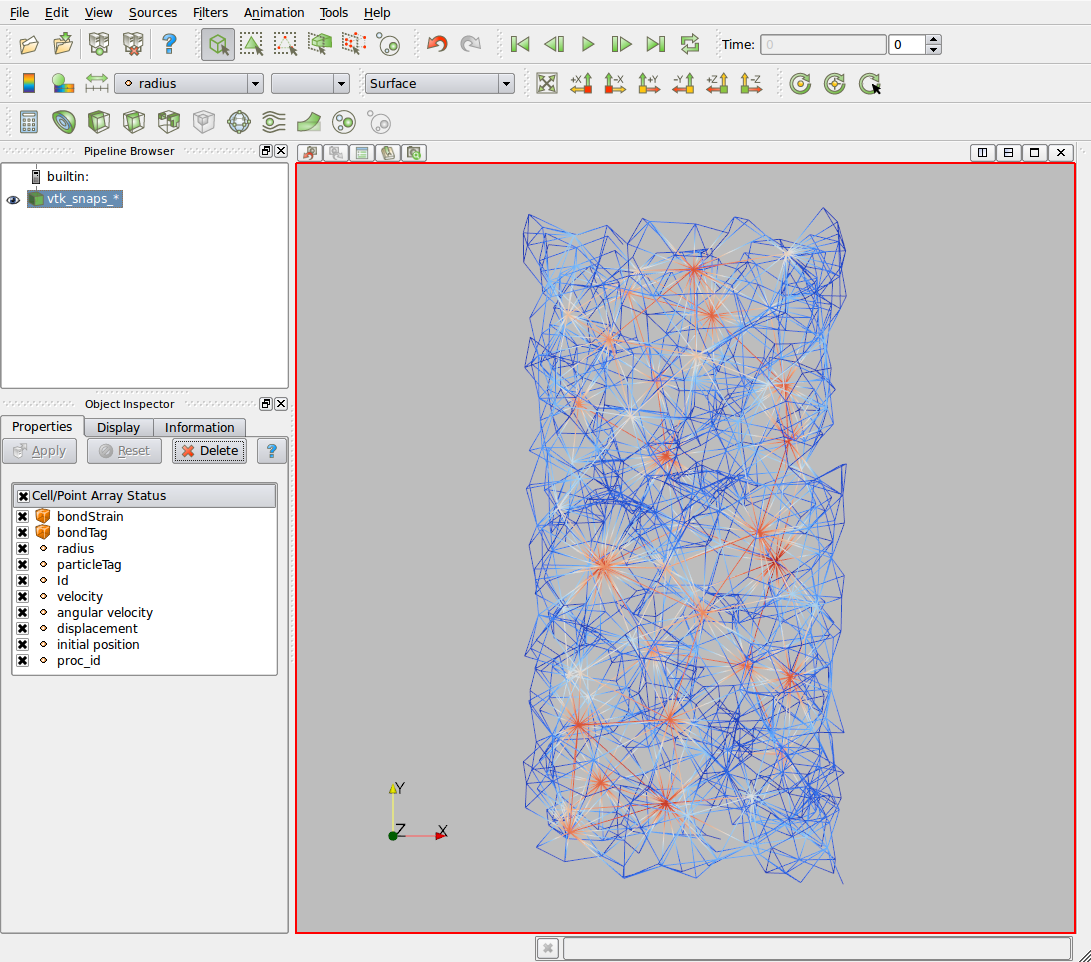
\includegraphics{PV_initial_window.png}}
\caption{An example of an ESyS-Particle simulation visualised using ParaView.} 
\label{fig:PV_initial_window}
\end{figure}


For this tutorial, we will focus on visualisation using ParaView to simplify discussion. VisIt is an equally good choice for visualising ESyS-Particle simulations, if you prefer it over ParaView.  The first step to interactively visualise ESyS-Particle simulation data is to convert the \texttt{CheckPoint} files into VTK unstructured mesh files. ESyS-Particle's \texttt{dump2vtk} post-processing tool is designed for this purpose.

\subsubsection{\texttt{dump2vtk}: convert checkpoint files to VTK files}

The following shell command will convert all of the \texttt{rot\_compress.py} \texttt{CheckPoint} files:

\begin{verbatim}
$ dump2vtk -i snapshot -o vtk_snaps_ -rot -t 0 251 1000
\end{verbatim}

\noindent
Having successfully executed this command, $251$ new files will be written to the directory containing the \texttt{CheckPoint} files. A partial directory listing of these files is as follows:

\begin{verbatim}
$ ls *.vtu
vtk_snaps_0.vtu
vtk_snaps_100.vtu
vtk_snaps_101.vtu
vtk_snaps_102.vtu
vtk_snaps_103.vtu
vtk_snaps_104.vtu
vtk_snaps_105.vtu
vtk_snaps_106.vtu
vtk_snaps_107.vtu
vtk_snaps_108.vtu
vtk_snaps_109.vtu
vtk_snaps_10.vtu
[...]
\end{verbatim}

\noindent
These new VTK files are in a suitable format for opening from within ParaView (\texttt{File | Open..}). Having opened the sequence of VTK files, you will be presented with a graphical window similar to Figure~\ref{fig:PV_initial_window}. 

\subsubsection{Interactive visualisation using ParaView}

The default graphical view in ParaView shows only the bonds linking particles, with the colours representing the radius of the particle residing at the intersection points of bonds. The VTK output files from \texttt{dump2vtk} contain a number of different scalar and vector fields that may be selected for visualisation via the \texttt{Display} tab in the \texttt{Object Inspector} pane to the left of the main ParaView window. The scalar and vector fields available for visualisation are:

\begin{itemize}
   \item scalar fields:
   \begin{itemize}
      \item \texttt{radius}: the radius of individual particles,
      \item \texttt{particleTag}: the tag assigned to each particle,
      \item \texttt{Id}: the unique identity number of each particle,
      \item \texttt{bondTag}: the tag assigned to individual bonds,
      \item \texttt{bondStrain}: an indication of the amount of strain stored in each bond,
      \item \texttt{proc\_id}: the unique worker process identity number for visualising parallel subdomain decomposition.
   \end{itemize}
   \item vector fields:
   \begin{itemize}
      \item \texttt{velocity}: the current velocity of each particle,
      \item \texttt{angular velocity}: the current angular velocity of each particle,
      \item \texttt{displacement}: the total displacement of each particle since the simulation commenced, and
      \item \texttt{initial position}: the initial position of each particle.
   \end{itemize}
\end{itemize}

In many cases, useful information can be gained by simply colouring the bonds according to one of the scalar fields above, or the magnitude of one of the vector fields. In other instances it is useful to use a so-called \texttt{Glyph} filter to visualise, for example, the velocity field as an assembly of arrows. Perhaps the most useful \texttt{Glyph} filter is the \texttt{Sphere} filter. This filter inserts a sphere at the location of each particle, the radius of which can be scaled by the particle radius. The spheres can then be coloured according to any of the fields listed above. Examples of visualising the particle assembly and a velocity field are provided in Figure~\ref{fig:PV_examples}.

ParaView also provides a group of controls on the toolbar that allows one to step through the sequence of VTK files in temporal order. Clicking on the \texttt{Play} symbol will automatically step through all the ($251$) snapshot files one at a time. In this manner, the progress of a simulation may be animated. There are also a number of other more advanced features of ParaView that are useful for visualisation of DEM simulation results. It is recommended that one explore ParaView and its documentation to learn about these features.

\begin{figure}
\resizebox{\textwidth}{!}{
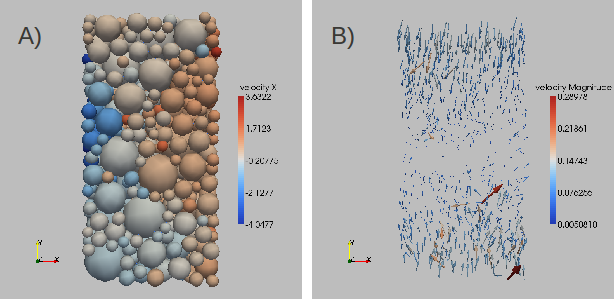
\includegraphics{PV_examples.png}}
\caption{Examples of visualisation using \texttt{Glyphs} in ParaView. A) Particles represented as sphere glyphs, coloured by the X-component of velocity; B) Particle velocities represented as arrow glyphs, coloured by the speed of each particle.}
\label{fig:PV_examples}
\end{figure}

\subsection{Calculating the number and size of rock fragments}

\subsubsection{\texttt{grainextract}: analysing rock fragments}

\subsubsection{Visualising rock fragments using ParaView}

\subsection{Visualising cracks formed during fracture simulations}

\subsubsection{\texttt{fracextract}: identifying locations of broken bonds}

\subsubsection{Visualising fractures using ParaView}

\subsection*{What's Next?}

In this tutorial some of the ESyS-Particle post-processing tools were introduced. One of these tools (\texttt{dump2vtk}) converts \texttt{CheckPointer} output files into VTK files, a popular 3D visualisation data format. Having converted checkpoint files to VTK format, third-party visualisation software can be used for advanced interactive visualisation of simulation results. Another post-processing tool (\texttt{grainextract}) permits analysis of the number and size of fragments produced during brittle failure simulations. In combination with \texttt{dump2vtk}, \texttt{grainextract} can also be used to interactively visualise the formation of fragments. The final post-processing tool to be considered was \texttt{fracextract} which calculates the locations and times of bond breakage events. Using this tool in combination with \texttt{dump2vtk} allows fracture patterns to be visualised. The ESyS-Particle post-processing tools are designed to permit advanced analysis and visualisation of simulation data with 
little additional computational expense over and above the burden required to execute simulations.

The following tutorial introduces another popular DEM simulation model, the annular shear cell. Shear cells are often employed in the laboratory to measure the bulk frictional response of sheared granular media. They are also popular for studying the fragmentation of granular media such as occurs within silos, along conveyor belts or within earthquake fault gouge zones. The purpose of the shear cell tutorial is to demonstrate some more features of ESyS-Particle and DEM simulations, namely how to conduct quasi-static two-dimensional simulations, how to implement periodic boundaries in one coordinate direction, and how to apply a constant external loading force to walls. These features are important weapons in the arsenal of a DEM modeller, finding application for simulating a broad range of physical phenomena.

\newpage
\section{Annular shear cells: quasi-static 2D simulations with periodic boundaries and servo walls}

In Chapter 6, uniaxial compression simulations were introduced for the purpose of calibrating the microphysical parameters of DEM models so that the macroscopic elastic properties match those of brittle-elastic materials such as rocks. Whilst uniaxial compression simulations (and their companions, tension and triaxial compression simulations) are quite useful for calibrating a DEM model to simulate brittle failure, such simulations are not as useful if one wishes to calibrate the model to simulate, for example, flow of granular material. 

One of the key macroscopic properties of granular media is the \emph{bulk friction coefficient}, defined as the effective frictional resistance of a volume of granular material under shear loading.  In the laboratory, the bulk friction coefficient is measured via either direct shear tests or annular shear cell tests. We will focus upon the later in this chapter. An annular shear cell consists of two metal rings, the bottom of which contains a groove within which is placed granular material (e.g. sand, gravel or powder). The top ring is then lowered onto the bottom ring and a series of weights and pulleys are used to maintain a constant vertical pressure on the ring of granular material. Subsequently the bottom ring is rotated at constant speed, thus shearing the granular material to a desired total shear strain. By measuring the force required to maintain a constant shearing rate, experimentalists can estimate the effective bulk friction coefficient of the granular material. 

\begin{figure}
\begin{center}
\resizebox{10cm}{!}{
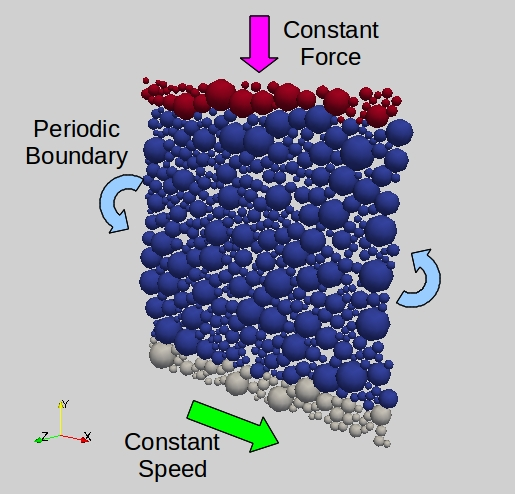
\includegraphics{ShearCellSetup.jpg}}
\end{center}
\caption{Diagram of a two-dimensional annular shear cell simulation employing periodic boundaries in the X-direction (from \texttt{shearcell.py}).} \label{fig:shearcell}
\end{figure}

In the following, we will discuss how to construct a two-dimensional version of the annular shear cell test using ESyS-Particle and demonstrate how the bulk friction coefficient may be calculated in shear cell simulations. The main purpose here is not to describe a production-ready DEM annular shear cell model suitable for calibration, but rather to elucidate a number of useful techniques in DEM modelling and how these are implemented in ESyS-Particle simulations.  As it happens, the annular shear cell is an ideal application with which to introduce these techniques within a practical context.  The key techniques we will discuss are:

\begin{itemize}
   \item how to restrict ESyS-Particle to two-dimensional computations,
   \item how to implement periodic (or circular) boundaries in one coordinate direction,
   \item how to conduct quasi-static simulations, and
   \item how to implement servo walls to maintain a constant external loading force (or stress) on a particle assembly.
\end{itemize}

Figure~\ref{fig:shearcell} illustrates the DEM model we wish to construct. It consists of a two-dimensional assembly of unbonded frictional particles of variable size. A layer of particles top and bottom are bonded elastically to planar walls that will act as driving plates. So as to simulate a ring of particles similar to the annulus of a shear cell, we employ periodic boundaries in the X-direction; particles exitting the model to the right will re-enter the model to the left and vice versa. A constant compressive force will be applied to the top driving plate in the negative Y-direction. In addition, the bottom plate will be moved at constant speed in the X-direction. Since annular shear cell tests are typically conducted under quasi-static conditions, we will also utilise two numerical approximations to achieve quasi-static conditions in the simulations, namely: 
\begin{enumerate}
   \item large viscous damping to remove elastic waves, and 
   \item higher than normal particle densities to ensure particle accelerations remain relatively small throughout the simulation.
\end{enumerate}

\noindent
The complete code-listing for the shear cell simulations may be found in Appendix~\ref{code:shearcell}.

\subsection{Two-dimensional computations and periodic boundaries}

For a number of applications, two-dimensional DEM simulations are sufficient to obtain useful results. Although ESyS-Particle is primarily designed with large, three-dimensional simulations in mind, it is relatively simple to instruct ESyS-Particle to ignore computations in the Z-direction, effectively reducing the simulation to two dimensions. The \texttt{LsmMpi.force2dComputations(..)} subroutine call achieves this. This subroutine call should be made very soon after initialising the simulation object (\texttt{LsmMpi}) and before setting the spatial domain of the simulation. The following code-fragment illustrates the use of \texttt{LsmMpi.force2dComputations(..)}:

\begin{verbatim}
#import the appropriate ESyS-Particle modules:
from esys.lsm import *
from esys.lsm.util import *
from esys.lsm.geometry import *

#create a simulation container object:
#       N.B. there must be at least two sub-divisions 
#       in the X-direction for periodic boundaries
sim = LsmMpi (numWorkerProcesses=2, mpiDimList=[2,1,1])
sim.initNeighbourSearch (
   particleType = "NRotSphere",
   gridSpacing = 2.5,
   verletDist = 0.5
)

#specify the number of timesteps and timestep increment:
sim.setNumTimeSteps(100000)
sim.setTimeStepSize(0.001)

#enforce two-dimensional computations:
sim.force2dComputations (True)
\end{verbatim}

ESyS-Particle also permits the use of periodic boundaries in one coordinate direction (the X-direction). Periodic boundaries in ESyS-Particle are implemented by borrowing the code used for managing transit of particles across parallel subdomain boundaries. Consequently, if one wishes to employ periodic boundaries, one must ensure there are at least two parallel subdivisions in the X-direction. In the code-fragment above, this is achieved by setting \texttt{mpiDimList=[2,1,1]} (and specifying the need for two worker processes via \texttt{numWorkerProcesses=2}). 

It is also necessary to inform ESyS-Particle that periodic boundaries are being used when one sets the spatial domain of the simulation. The code-fragment below illustrates how this is done:

\begin{verbatim}
#specify the spatial domain and direction of periodic boundaries:
domain = BoundingBox ( Vec3 (0,0,0), Vec3 (10,10,0) )
sim.setSpatialDomain (
   bBox = domain,
   circDimList = [True, False, False]
)
\end{verbatim}

Having assigned the appropriate number of parallel subdivisions and correctly set the \texttt{circDimList} argument of \texttt{LsmMpi.setSpatialDomain(..)}, the simulation object is initialised to employ periodic boundaries in the X-direction. A simple test script could easily be constructed in which a single particle is inserted with an initial velocity in the X-direction. As the simulation progresses the particle would simply loop around and around the X-direction, exiting one side of the domain and re-entering the other side. If periodic boundaries were not correctly initialised, the particle would simply disappear from the simulation once it crossed the spatial domain boundary.

For our annular shear cell simulation, we desire a particle assembly consisting of particles of variable size, initially at random locations. As we have seen in previous tutorials, the \texttt{RandomBoxPacker} can be used for this. So that we achieve a dense initial particle packing, the \texttt{RandomBoxPacker} must also be informed of the presence of periodic boundaries. The following code-fragment illustrates:

\begin{verbatim}
#construct a rectangle of unbonded particles:
packer = RandomBoxPacker (
   minRadius = 0.1,
   maxRadius = 0.5,
   cubicPackRadius = 2.2,
   maxInsertFails = 1000,
   bBox = BoundingBox(
      Vec3(0.0, 0.0,0.0),
      Vec3(10.0, 10.0, 0.0)
   ),
   circDimList = [True, False, False],
   tolerance = 1.0e-5
)
packer.generate()
particleList = packer.getSimpleSphereCollection()
\end{verbatim}

\noindent
Note that we have not yet inserted the particles into the simulation object. This is because we wish to tag the particles carefully prior to insertion, as explained in the next section.

\subsection{Quasi-static simulations: local damping and high densities}

Annular shear cell experiments in the laboratory are typically conducted under so-called \emph{quasi-static} conditions. Mathematically, quasi-static conditions imply that particle accelerations are negligible and, hence, inertial effects (such as elastic wave propagation) are neglected. ESyS-Particle employs an explicit finite-difference time-integration scheme in which particle velocities and positions are updated by computing the instantaneous acceleration of each particle (via Newton's Second Law). Such a time-integration scheme is only suitable for \emph{dynamic} conditions in which the accelerations are non-zero. If all particle accelerations were zero, no stationary particles would move and non-stationary particles would move at constant speed (Newton's First Law). 

One way to simulate quasi-static conditions in a DEM model would be to change the time-integration scheme to an implicit (typically iterative) scheme in which particle positions and forces are repeatedly updated until all forces are negligible. To implement such a scheme in ESyS-Particle would require significant re-factoring of the DEM engine and is likely to be quite computationally inefficient. An alternative approach that is often adopted by DEM practitioners involves the use of two numerical approximations that together achieve quasi-static conditions. 

The first numerical approximation is known as the \emph{high density approximation}. It involves assigning unrealistically large densities (or masses) to all particles. Since the instantaneous acceleration of a particle is inversely proportional to its mass ($a = F/m$), a larger mass results in a smaller acceleration, for a given net force acting on a particle. Here the particle mass is being used as a type of \emph{penalty factor} to reduce the amplitudes of particle accelerations. However, given that the particle accelerations will never be zero, some inertial effects will be expected to remain. 

The second numerical approximation, large artificial damping, attempts to reduce the impact of these inertial effects. By utilising a relatively large amount of viscous damping, elastic waves can be efficiently reduced in amplitude over a few time-steps. In this way inertial effects can also be managed to achieve effectively quasi-static conditions in the DEM simulations. 

To implement the high density approximation in ESyS-Particle simulations, we must prescribe large particle densities. The \texttt{LsmMpi.setParticleDensity(..)} subroutine achieves this. As this subroutine sets the density of all particles with a given tag, we must first assign a tag to each particle before insertion into the simulation object. Later we will need to bond a layer of particles top and bottom to driving plates, so we will need three particle tags: one for unbonded particles within the cell (\texttt{tag=1}), one for particles near the bottom plate (\texttt{tag=2}) and one for particles near the top plate (\texttt{tag=3}). The following code-fragment tags the particles accordingly and inserts them into the simulation:

\begin{verbatim}  
#tag particles along base and top of rectangle
#then add the particles to the simulation object:
for pp in particleList:
   centre = pp.getPosn()
   radius = pp.getRadius()
   Y = centre[1]
   if (Y < 1.0):                # particle is near the base (tag=2)
      pp.setTag (2)
   elif (Y > 9.0):              # particle is near the top (tag=3)
      pp.setTag (3)
   else:                        # particle is inside the shear cell (tag=1)
      pp.setTag (1)
   sim.createParticle(pp)       # add the particle to the simulation object
\end{verbatim}  

Having assigned a tag to each particle, the density of the particles can be set using the following syntax:

\begin{verbatim}
#set the density of all particles:
sim.setParticleDensity (
   tag = 1,
   mask = -1,
   Density = 100.0
)
\end{verbatim}

\noindent
Remember to also set the density of particles with \texttt{tag=2} and \texttt{tag=3} using similar subroutine calls.

In previous tutorials, the \texttt{LinDampingPrms} artificial viscosity Interaction Group has already been encountered. By assigning a relatively large value for the \texttt{viscosity} parameter, we can use \texttt{LinDampingPrms} to damp inertial effects. The following code-fragment achieves this in our shear cell simulation:

\begin{verbatim}
#add local damping to avoid accumulating kinetic energy:
sim.createInteractionGroup (
   LinDampingPrms (
      name = "damping",
      viscosity = 1.0,
      maxIterations = 100
   )
)
\end{verbatim}

Due to the way ESyS-Particle implements damping, it is important that the specification of damping interaction groups is placed after that of all other interaction groups in a simulation script. Before adding the code-fragment above to your script, insert the following:

\begin{enumerate}
   \item two walls above and below the particle assembly (at $Y=0$ and $Y=10$),
   \item \texttt{NRotFrictionPrms} interactions between unbonded particles, and
   \item \texttt{NRotBondedWallPrms} to bond appropriately tagged particles to the walls.
\end{enumerate}

\noindent
Once you have added these items and the \texttt{LinDampingPrms} interaction group to your script, we are ready to define the boundary conditions. The next section describes how to do this.

\subsection{Servo walls and constant stress boundary conditions}

As described in the introduction to this chapter, annular shear cells are loaded via a combination of a constant vertical confining pressure applied to the top ring and shear of the bottom ring at a constant rate. To simulate shear at a constant rate, we can simply re-use the \texttt{WallLoaderRunnable} we encountered in Chapter 6. So as to match the typical laboratory conditions, we will only shear the \texttt{bottom\_wall}. The following code-fragment achieves that:

\begin{verbatim}
#import the WallLoaderRunnable (at the top of the script):
from WallLoader import WallLoaderRunnable

[...]

#add WallLoaderRunnables to shear the bottom driving plate:
wall_loader1 = WallLoaderRunnable(
   LsmMpi = sim,
   wallName = "bottom_wall",
   vPlate = Vec3 (0.125, 0.0, 0.0),
   startTime = 30000,
   rampTime = 10000
)
sim.addPreTimeStepRunnable (wall_loader1)
\end{verbatim}

\noindent
Notice that the wall is moved in the X-direction this time and that shear does not commence until $30000$ timesteps have elapsed. The delay commencing shear is to provide sufficient time to apply a constant vertical stress to the model, via the \texttt{top\_wall}. 

Now that we have implemented constant shear boundary conditions for the \texttt{bottom\_\+wall}, we must also implement a constant vertical stress loading condition on the \texttt{top\_wall}. In DEM simulations, constant boundary forces (or stresses) are implemented via so-called \emph{servo walls}. A servo wall is a wall that is incrementally moved a small distance in order to maintain a constant prescribed net force acting on the wall. The net force on a wall is a combination of the forces due to all particles interacting with the wall and any external forces (or applied motions). Consequently, in order to compute the wall displacement required to maintain a prescribed net force, one must have access to all the instantaneous particle-wall forces. Of course, once the wall is moved, these particle-wall forces change, so one must recompute the net force on the wall. Typically a simple iterative procedure can be employed in which a wall is moved a small distance, forces are recomputed, then the wall is moved 
again. In most circumstances, this iterative procedure converges rapidly and the loop is terminated when the incremental wall displacement is smaller than a prescribed tolerance. 

Although it is technically possible to implement a servo wall algorithm from within a \texttt{Runnable}, this would be computationally inefficient, requiring numerous communications between the Python API, the master process and the workers. Consequently, ESyS-Particle provides a built-in subroutine, \texttt{LsmMpi.applyForceToWall (..)}, that implements a simple servo wall algorithm. The user need only supply the \emph{name of the Interaction Group} specifying the type of particle-wall interactions, as well as the net force to apply to the wall. The following code-fragment illustrates how one might apply a $1N$ force in the Y-direction to the \texttt{top\_wall} in our shear cell simulation:

\begin{verbatim}
sim.applyForceToWall (
   interactionName = "twall_bonds", 
   force = Vec3 (0,1,0)
)
\end{verbatim}

\noindent 
Note that we do not supply the name of the wall but rather the particle-wall interaction group, \texttt{twall\_bonds}.

In order to maintain quasi-static equilibrium in the shear cell simulations, it is advantageous to initially increase the applied force linearly until the desired force is achieved. This is similar to the initial acceleration implemented in the \texttt{WallLoaderRunnable}. A \texttt{Runnable} that achieves this, called \texttt{ServoWallLoader.py}, is provided in Appendix~\ref{code:ServoWallLoader}. Once implemented, all that remains is to import and initialise this \texttt{Runnable} in \texttt{shearcell\+.py}:

\begin{verbatim}
#import the ServoWallLoaderRunnable (at the top of the script):
from ServoWallLoader import ServoWallLoaderRunnable

[...]

#add ServoWallLoaderRunnables to apply constant normal stress:
servo_loader1 = ServoWallLoaderRunnable(
   LsmMpi = sim,
   interactionName = "twall_bonds",	
   force = Vec3 (0.0, -1000.0, 0.0),
   startTime = 0,
   rampTime = 5000
)
sim.addPreTimeStepRunnable (servo_loader1)
\end{verbatim}

\noindent
The arguments to \texttt{ServoWallLoaderRunnable} instruct ESyS-Particle to linearly increase the applied force on the \texttt{top\_wall} for $5000$ timesteps, then maintain a constant vertical force of $1000N$ thereafter. Recall that shear commences after $30000$ timesteps, so there is plenty of time for the model to equilibriate at the desired confining pressure prior to shear commencing.

Now that the two boundary conditions are implemented, the physics of the shear cell model are complete. Of course, it would be advantageous to include some \texttt{FieldSavers} or a \texttt{CheckPointer} prior to commencing a simulation. The next section describes how to use \texttt{WallVectorFieldSavers} to measure the bulk friction coefficient of the sheared unbonded particles, as well as how to observe whether dilation occurs during shear.

\subsection{Computation of bulk frictional properties of granular media}

The primary purpose of DEM shear cell simulations is to provide a means to calibrate the microphysical model parameters so that the bulk frictional properties of the DEM model match those measured in laboratory experiments. In the laboratory, the bulk friction coefficient of a sheared granular material is estimated by measuring the amount of force (or torque) required to maintain a constant rate of shear at the boundaries. The bulk friction coefficient ($\mu_{\mathrm{bulk}}$) is defined as the measured shear force ($F_s$) divided by the applied normal force ($F_n$) i.e.

\[ \mu_{\mathrm{bulk}} \approx \frac{F_s}{F_n} \]

\noindent
Typically a time-series of the bulk friction coefficient is averaged in order to obtain a measure of the mean bulk friction coefficient. The standard deviation provides a measure of the degree of variability of the bulk friction. 

It should be obvious that in order to estimate the bulk friction coefficient in the DEM shear cell simulations, we need to extract time-series of the forces acting on the walls throughout the simulations. The following \texttt{WallVectorFieldSaver} will provide the necessary raw data:

\begin{verbatim}
force_saver = WallVectorFieldSaverPrms(
   wallName=["bottom_wall", "top_wall"],
   fieldName="Force",
   fileName="out_Force.dat",
   fileFormat="RAW_SERIES",
   YbeginTimeStep=0,
   endTimeStep=100000,
   timeStepIncr=1
)
sim.createFieldSaver(force_saver)
\end{verbatim}

\noindent
This code-fragment should be quite familiar as it is almost identical to that used in the \texttt{rot\_compress.py} tutorial. 

\begin{figure}
\begin{center}
\resizebox{10cm}{!}{
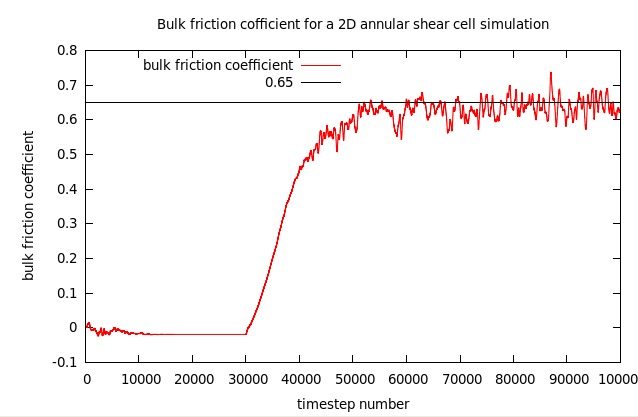
\includegraphics{SC_bulk_friction.png}}
\end{center}
\caption{Time-series of the effective bulk friction coefficient from a two-dimensional annular shear cell simulation (from \texttt{shearcell.py}).} \label{fig:bulkFriction}
\end{figure}

A time-series of the bulk friction coefficient from a shear cell simulation is provided in Figure~\ref{fig:bulkFriction}. In this figure we average the normal and shear forces acting on the two walls as measures for $F_n$ and $F_s$ in the formula above. Note that during the initial stage of the simulation, the bulk friction coefficient is near-zero. During this interval only a normal force is applied to the top wall (with no shear applied to the bottom wall). Once shear commences (after $30000$ timesteps) the bulk friction coefficient rapidly rises to approximately $\mu_{\mathrm{bulk}} \approx 0.65$. Thereafter, rough stable sliding of the granular material ensues, with the bulk friction coefficient remaining near-constant.

This result is typical when shearing a granular material comprised of irrotational spheres with a constant internal friction coefficient (here we set the internal friction coefficient as $0.6$). Past research has demonstrated that inhibiting rolling of DEM particles (through the use of \texttt{NRotSpheres}) results in a bulk friction coefficient that increases as the internal friction coefficient increases. However, when rotational, unbonded particles are used, the bulk friction coefficient is significantly smaller, and almost independent of the choice of internal friction coefficient. 

The reason for this is that spheres simply roll over one another without any geometrical interlocking and, more importantly, without \emph{dilation} of the granular material as it shears. A time-series of the top wall position (as shown in Figure~\ref{fig:dilation}) confirms that the top wall monotonically reduces in height throughout the simulation. If geometrical interlocking had occurred, one would expect to see evidence for the top wall ``riding up'' as the granular material becomes locally interlocked.  Thankfully there is a relatively simple way to achieve realistic frictional response in DEM shear cell simulations: utilise clusters of particles bonded together that interlock by virtue of the surface roughness of the clusters. In the next chapter we will discuss how one might construct a shear cell model incorporating clusters of bonded particles representing the granular material. 

\begin{figure}
\begin{center}
\resizebox{10cm}{!}{
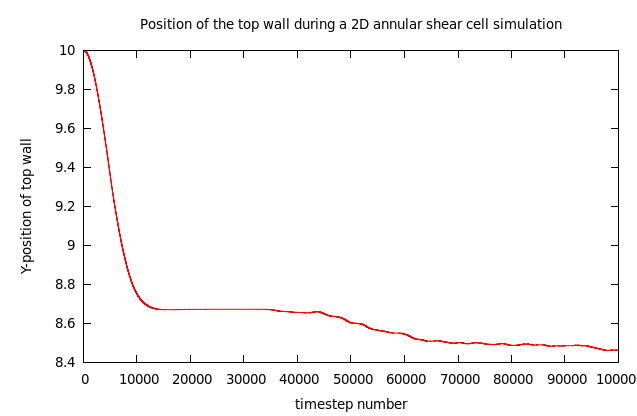
\includegraphics{SC_dilatancy.png}}
\end{center}
\caption{Time-series of the top wall position from a two-dimensional annular shear cell simulation (from \texttt{shearcell.py}).} \label{fig:dilation}
\end{figure}

\subsection*{What's Next?}

In this chapter, a number of useful DEM modelling techniques were introduced using annular shear cell experiments as a motivation. We discussed how to conduct two-dimensional simulations with ESyS-Particle, including periodic boundaries in one coordinate direction. The use of large viscosity and high particle densities was demonstrated as an effective method to achieve quasi-static conditions in DEM simulations without altering the time-integration scheme. Servo walls were also discussed as a mechanism to apply constant boundary forces (or stresses) to DEM models. 

In the final section of this chapter, we analysed some results from the simple shear cell model. These results, although promising, demonstrated a lack of geometrical interlocking, an important mechanism governing the frictional response of granular media. Some DEM practitioners have implemented more complicated particle-pair interactions to overcome this limitation. This is often a reasonable compromise when computational resources are limited. Another approach is simply to make the model geometrically more complex without increasing the mathematical complexity of the particle-pair interactions. Past research using ESyS-Particle has demonstrated that the use of bonded clusters of particles to represent individual grains results in bulk frictional response matching that observed in laboratory experiments. 

There are numerous other instances where increasing the geometrical realism of a DEM model can yield more realistic results without resorting to more complicated interaction laws. This observation is one of the reasons ESyS-Particle is designed for use on parallel supercomputers. Increased geometrical realism typically requires the use of significantly larger numbers of particles. ESyS-Particle permits these significantly larger models to be executed on parallel supercomputers in almost the same amount of time as a smaller model on a desktop PC. 
As simulation models become increasingly complex, one may need to carefully design models to achieve optimal performance or make use of third party tools to generate and analyse these models. The following chapter describes some of the other resources available to assist advanced users of ESyS-Particle.

Of course, in order to construct these geometrically complex models, one requires a flexible tool for model construction. The next chapter introduces \texttt{GenGeo}, a companion library to ESyS-Particle, designed as a tool for constructing DEM models that are much more geometrically complex than we have encountered thus far.

\section{Stopping and restarting simulations}

In ESyS-Particle it is possible to save the state of a simulation at a given time and to restart it from that state. This can be quite useful in a number of situations, in particular for long running simulations. Examples would be simulations which exceed run time limits on HPC systems or the recovery after a system failure. There are, however, a couple of limitations to this. The  main ones are 
\begin{enumerate}
 \item There is no guarantee whatsoever that simulations saved using one version of ESyS-Particle can be restarted using another version. 
 \item The simulations need to be restarted using the same number of worker processes as the original simulation
 \item Due to the limited precision of the saved data\footnote{The data mostly consists of variables of type \texttt{double} in the running simulation but is saved in ASCII format with 12 significant digits in the mantissa.} there will be small differences between the saved and the restored state of the  simulations.
 \end{enumerate} 
The 3rd issue means that some aspects of restarted simulations will, in some cases, start to diverge slowly from the original run. If this happens it is usually a sign that the affected aspect(s) of the model which is/are highly sensitive to the initial conditions. Should the particular aspect(s) be an important outcome of the simulation it would therefore be advisable to run ensemble simulations anyway.     \\
Key components for the realization of this mechanisms are the creation of restartable checkpoints via \texttt{createRestartCheckPointer} and the function \texttt{loadCheckPoint}. The restart checkpoints are similar to the snapshots described in section \ref{sec:postprocessing}, in particular the initialization of the \texttt{RestartCheckPointPrms} class takes the same arguments as the \texttt{CheckPointPrms} class. Therefore the saving of restart checkpoints can be set up by adding the follwing code fragment the time simulation script.
\begin{verbatim}
sim.createRestartCheckPointer (
   RestartCheckPointPrms (
      fileNamePrefix = "checkpoint",
      beginTimeStep = 0,
      endTimeStep = 250000,
      timeStepIncr = 10000
   )
)
\end{verbatim}  
Note that the only difference between this and the saving of snapshots for postprocessing is the additional \"Restart\" in the names of the checkpointer and its parameter class.     




\newpage

%% ---
%% GenGeo Section
%% ---
\chapter[GenGeo]{Jazzing things up: complicated particle geometries using \texttt{GenGeo}}

\section{A short introduction to \texttt{GenGeo}}
The \texttt{GenGeo} library is build around three basic concepts:
\begin{itemize}
\item geometrical volumes to fill with particles  
\item a "Packer" to place the particles into the volumes according to given criteria 
\item the "Neighbour Table" - a container to store the particles and to keep track of their relative positions and neighbour relations 
\end{itemize}

\subsection{Volumes}

\subsection{Packers}
While the library is designed to be flexible and to allow many different packing methods to be included the only packers implemented at the moment are all based to the insertion-based algorithm described in (REF). The advantages of this packing strategy are that it produces relatively dense particle arrangements where each interior particle is touched by at least 4 other particles in 3D (by 3 other particles in 2D) and that there are no frozen-in stresses between the particles. The disadvantage is that the user can not control the particle size distribution except for the minimum and maximum particle radius allowed.  

\subsection{Neighbour Tables}
- Verlet \\
- 2D/3D \\
- Circular Boundaries \\

\section{Particles in a box: a simple \texttt{GenGeo} example}
\label{sec:simple_box}

This section introduces the basic features of \texttt{GenGeo} using a very simple example: filling a box with particles. The resulting particle packing is similar to that produces inside the ESyS-particle simulation described in section \ref{sec:block_in_sim}. However, given that it is saved to a file it can be re-used for multiple simulations. The full code for the example is available in Appendix~\ref{geocode:box}. N.B. To make the meaning of the function arguments clear the "named argument" style of python function calls will be used in the sections explaining the \texttt{GenGeo} example. However, to improve general readability the compact form, i.e. without argument names, will be used for the full listings in the appendix. \par
Like most simple \texttt{GenGeo} scripts this example consists of 5 steps:
\begin{enumerate}
\item setting up a neighbour table
\item defining the volume to be filled - i.e. the box
\item setting up the packer
\item running the packer to fill the box and, if required, bond the particles together
\item write the particle data to an output file 
\end{enumerate}  
As usual, the thing to do in a python script is to import the necessary modules, therefore the script to pack particles into a box starts with 
\begin{verbatim}
from gengeo import *
\end{verbatim}
which of course assumes that the  \texttt{GenGeo} library \footnote{Despite the fact that it is spelled \texttt{GenGeo} throughout this tutorial, the actual module name is all lower case \texttt{gengeo}, i.e. on Unix systems the shared library name is gengeo.so } is in the python path. In order to make the code more readable we first define a couple of parameters which will be needed repeatedly throughout the script, namely the dimensions of the box we intent to fill and the minimum and maximum radius of the particles. For simplicity we place one corner of the box at (0.0,0.0,0.0) so we only need to specify the x-, y- and z- extent of the box to define it fully \footnote{The "Box" volumes, both in 2D and in 3D, only support boxes with edges parallel to the coordinate axes. Non-axis aligned boxes can be defined using a convex polyhedron volume.}. So the next section of the script looks like this:
\begin{verbatim}
# box dimensions
xdim=10
ydim=20
zdim=10

# particle size range
minRadius = 0.2
maxRadius = 1.0
\end{verbatim}
This will set the shape of the box to a square prism two times as long as wide. This shape is quite often used, for example in simulations of triaxial deformation tests. With the parameters given here the resulting model will be relatively small ($\approx 4000$ particles) and should build in about 10 - 20 seconds on current PC \footnote{Tested $\approx 16$ seconds on an Intel Core2 Q9300 (2.5GHz)}. For convenience we also define the two opposing corners of the box as vectors. N.B. In \texttt{GenGeo} the class for a 3D vector is called \texttt{Vector3}, \emph{not} \texttt{Vec3} as in ESyS-Particle! The reason for this difference is to avoid name conflicts when using both \texttt{GenGeo} and ESyS-Particle libraries in the same Python script. So the definition of the corner points is
\begin{verbatim}
# corner points
minPoint = Vector3(0.0,0.0,0.0)
maxPoint = Vector3(xdim,ydim,zdim)
\end{verbatim}
Now the corner points can be used to define both the volume to be filled and the neighbour table to contain the particles. The volume, which is of the class \texttt{BoxWithPlanes3D} takes exactly two parameters in its constructor, describing the locations of two opposite corners of the box. Therefore both parameters are of type \texttt{Vector3}. The class name \texttt{BoxWithPlanes3D}, in particular the "WithPlanes" part will become clearer in the next section \ref{sec:gengeo_box2}.
So to set up the box we use the previously defined corner points
\begin{verbatim}
# block volume
box = BoxWithPlanes3D(
    minPoint=minPoint,
    maxPoint=maxPoint
    )
\end{verbatim}
Next we need a neighbour table to store the particles. The constructor for the neighbour table takes 4 arguments: two corner points (\texttt{minPoint}, \texttt{maxPoint}) to describe the volume covered by the model, the grid spacing (\texttt{gridSize}) and the number of particle groups (\texttt{numGroups}). The volume covered by the neighbor table should ideally be the bounding box of the whole model, i.e. it needs to cover all particles but it should not be much larger in order to minimize the memory used. The grid spacing determines the search range used for the determining if two particles touch each other. To make sure all touching (or intersecting) pairs of particles can be found the grid spacing needs to be larger than twice the maximum particle radius. The number of particle groups will only be different from 1 for rather complicated geometry set-up scripts, so we set numGroups=1 here. So the construction of the neighbor table looks as follows:
\begin{verbatim}
# neighbour table 
mntable = MNTable3D(
    minPoint=minPoint,
    maxPoint=maxPoint,
    gridSize=2.5*maxRadius,
    numGroups=1
    )
\end{verbatim}
Next we need to set up the "packer" which places the particles inside the volume. As we want to pack single particles in 3D we chose a packer of type \texttt{InsertGenerator3D}. The most simple constructor for this type of packer takes 5 arguments. In addition to the minimum and maximum particle radius (\texttt{minRadius}, \texttt{maxRadius}) there are 3 parameters which control the performance of the packing algorithm. These are the number of consecutive failed particle insertion attempts allowed before the algorithm gives up and terminates(\texttt{insertFails}), the maximum number of iterations for the internal sphere fitting procedure (\texttt{maxIterations}) and the precision of the sphere fitting, i.e. the maximum tolerance up to which two particles are still considered touching (\texttt{tolerance}). The values we use here, \texttt{insertFails=1000}, \texttt{maxIterations=1000} and \texttt{tolerance=1e-6} usually work fine for small to medium models. For large models it can be necessary to increase the value of \texttt{insertFails} to obtain a good packing. The value of \texttt{tolerance} should be considered in relation to the particle radii. A sixth parameter \texttt{seed} can be used to force a re-seeding of the random number generator before the packing algorithm starts.  Setting \texttt{seed=True} guarantees a different packing with each run of the script, what happens otherwise is system-dependent. Taking this all into account the packer is constructed like this:
\begin{verbatim}
# packer
packer = InsertGenerator3D(
    minRadius=minRadius,
    maxRadius=maxRadius,
    insertFails=insertFails,
    maxIterations=maxIter,
    tolerance=tol
    )
\end{verbatim}
Now that the volume, the neighbour table and the packer, are defined the actual work can start. First the packer needs to fill the volume with particles. In the simplest case this requires two arguments to the \texttt{generatePacking} function of the packer: the volume to fill and the neighbour table in which to store the particles. Therefore the function call to fill the "box" volume with particles is
\begin{verbatim}
# pack particles into volume
packer.generatePacking(
    volume=box,
    ntable=mntable
    )
\end{verbatim} 
The last thing to do to complete the generation of the particle arrangement is to create the bonds between touching particle pairs. Because the neighbour table contains all informations necessary to determine which particles should be bonded, i.e. particle positions and radii, the bonding procedure is a member function of the neighbour table. The most simple form of the function call, which just bonds all neighbouring particles in on group, needs 3 arguments: the ID of the particle group which should be bonded \texttt{groupID}, the bonding tolerance \texttt{tolerance} and the tag given to the newly created bonds \texttt{bondID}. Because our neighbour table contains only one group of particles, we need to set \texttt{groupID=0}. The tolerance for bonding should normally be larger than the packing tolerance used in the packer, so we chose 1e-5 here. The bond tag can be set to any value, but given that we only have one set of bonds in this model we may as well use 0. So the call to create the bonds looks as follows:  
\begin{verbatim}
# create bonds between neighbouring particles:
mntable.generateBonds(
    groupID=0,
    tolerance=1.0e-5,
    bondID=0
    )
\end{verbatim}
And after this the model is fully built. The only thing left to do is to write the model data into a file so it can be used. For this purpose the neighbour table has a \texttt{write} function which can write the information stored in the neighbour table, i.e. particles and bonds, to a file in different ways which are controlled by the \texttt{outputStyle} argument. If \texttt{outputStyle=1} a "geo" file is written which can be used in ESyS-Particle scripts, if  \texttt{outputStyle=2} a VTK file \footnote{Specifically a VTK-XML unstructured grid file - see the documentation of VTK toolkit on www.vtk.org for more details on the file format.} is written for the use with visualisation software such as Paraview(tm). Of course the \texttt{write} function also needs the file name as first argument, so to write both a geo and a VTK file the calls should be:
\begin{verbatim}
# write a geometry file
mntable.write(
    fileName="box.geo", 
    outputStyle=1
    )
mntable.write(
    fileName="box.vtu",
    outputStyle=2
    )
\end{verbatim}   
which concludes the \texttt{GenGeo} script to generate a box filled with bonded particles. The script can now be executed as usual, i.e. \texttt{python\ simple\_box.py}. During execution there will be some debug output, in particular for every 100 particles inserted \texttt{GenGeo} will output a line stating how many particles have been inserted so far \footnote{This number does not include the particles generated during the "seeding" stage of the algorithm} and how many attempts it took on average to insert one of the last 100 particles. When the execution of the script finishes it should have produces two files, "box.geo" and "box.vtu". When visualized with Paraview the result should look similar to that shown in Figure \ref{fig:simple_box}.  
%% --- Fig simple_box
\begin{figure}
\begin{center}
\resizebox{2.5in}{!}{
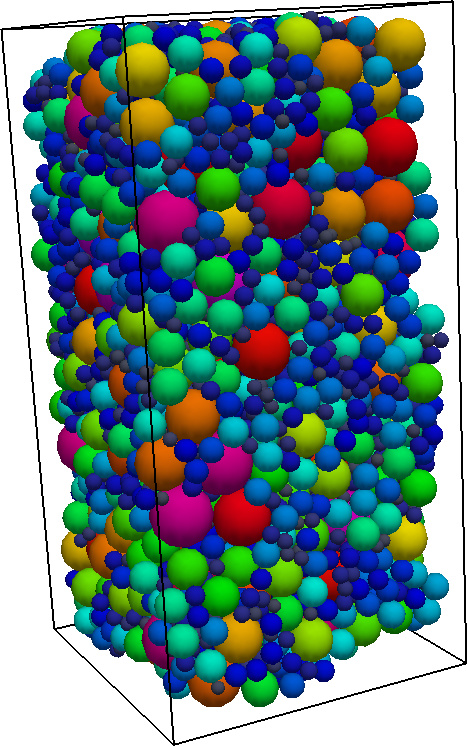
\includegraphics{gengeo_box.jpg}}
\end{center}
\caption{An image (generated with Paraview) of the box filled with particles generated by the script \texttt{simple\_box.py} described in section \ref{sec:simple_box} } \label{fig:simple_box}
\end{figure}
%% -----
One issue which is noticeable with this model is that the surfaces, and particularly the edges, are rough, rather than smooth. How to overcome this is described in the next section.

\section{Particles in a box Mk II: making the the boundaries smooth(er)}
\label{sec:gengeo_box2}
The reason why the walls of the box generated in the previous section are not as smooth as expected is that the \texttt{InsertGenerator} uses the box volume only determine if a particle is inside the volume or not, it does not fit particles to the faces of the box. This can be changed by adding some \texttt{Plane} objects to the box volume. To do this, it is necessary to define the planes first. Each \texttt{Plane} object is defined by a point on the plane and the normal direction of the plane. To add a  \texttt{Plane} object for each face of the box a total of 6 planes are needed, three passing through the point (0,0,0), which is called \texttt{maxPoint} in the script described in the previous section, with normals pointing in the positive x-, y- and z-direction and three passing through the opposite corner of the box, which was called \texttt{maxPoint} in the script. So the definition of a plane parallel to the xy-plane, i.e. with a normal pointing in the z-direction, and going through the point "minPoint" is
\begin{verbatim}
bottomPlane=Plane(
    origin=minPoint,
    normal=Vector3(0.0,0.0,1.0)
)
\end{verbatim} 
The other 5 planes can be defined in the same way or, more compact, by the following lines:
\begin{verbatim}
leftPlane=Plane(minPoint,Vector3(1.0,0.0,0.0))
frontPlane=Plane(minPoint,Vector3(0.0,0.0,1.0))
topPlane=Plane(maxPoint,Vector3(0.0,-1.0,0.0))
rightPlane=Plane(maxPoint,Vector3(-1.0,0.0,0.0))
backPlane=Plane(maxPoint,Vector3(0.0,0.0,-1.0))
\end{verbatim}
To enable the packer to fit the particles to the planes when filling the box volume the \texttt{Plane} objects need to be added to the \texttt{BoxWithPlanes3D} object by using its \texttt{addPlane} member function. This function takes a \texttt{Plane} object as its only argument. To add the bottomPlane defined above to the box volume the call is 
\begin{verbatim}
box.addPlane(
    Plane=bottomPlane
)
\end{verbatim}
and for the other five planes, in the compact form,
\begin{verbatim}
box.addPlane(leftPlane)
box.addPlane(frontPlane)
box.addPlane(topPlane)
box.addPlane(rightPlane)
box.addPlane(backPlane)
\end{verbatim}
If these lines are added \ref{sec:simple_box} somewhere between the definition of the box volume and the call to generate the particle packing in the simple script filling a box which was developed in the previous section we have the complete script to generate a box full of particles where the sides are as smooth as possible for the given particle size range. The full code for the example is available in Appendix~\ref{geocode:smooth_box}. The resulting model can be seen in Figure \ref{fig:smooth_box} A). If the surfaces are still too rough for a particular application the smoothness can be improved by extending the range of particle sizes towards smaller radii. This can easily be achieved in the script described here by changing the variable \texttt{minRadius} to an appropriate value. The result of setting  \texttt{minRadius=0.05} is shown in Figure \ref{fig:smooth_box} B). \par	

%% --- Fig smooth_box
\begin{figure}
\begin{center}
\resizebox{120mm}{!}{
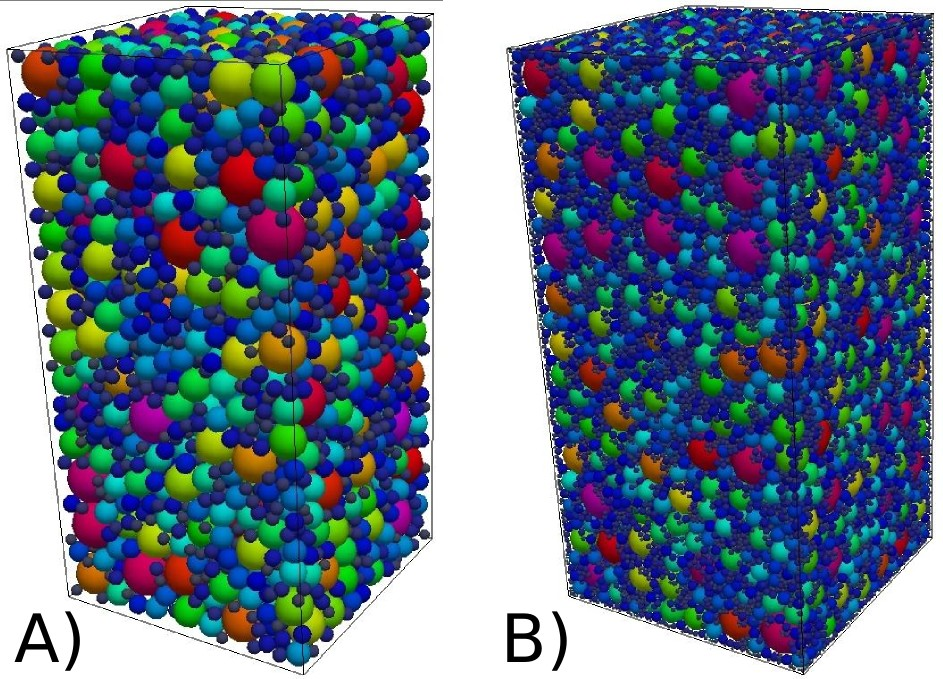
\includegraphics{smooth_box.jpg}}
\end{center}
\caption{Images (generated with Paraview) of a box with particles fitted to the box faces generated by the script \texttt{smooth\_box.py} described in section \ref{sec:gengeo_box2}. The model in A) uses particle radii between 0.2 and 1.0, the model in B) uses particle radii between 0.05 and 1.0.} \label{fig:smooth_box}
\end{figure}
%% -----

\subsection{Smoothness, particle sizes and particle numbers}

However, while smooth surfaces and dense particle arrangements can be realized with packings using wide size distribution of particles, i.e. a large ratio $r_{max} : r_{min}$ it should also be noted that this leads to a significant increase in the number of particles for the same model size. A very rough estimate would be that for a given maximum particle size the total number of particles in a volume goes up approximately as $n_p \approx 1 / {r_{min}}^2 $ \footnote{The exact relationship between model volume, particle size range and particle number is more complicated, particularly for relatively narrow particle size ranges. However, the $ 1 / {r_{min}}^2 $ relationship is a usable rule of thumb. N.B. This applies for \textbf{fixed} $\mathbf{r_{max}}$  - for fixed $ r_{max} / r_{min} $  the relation is obviously  $n_p \approx 1 / r^3 $ } where $n_p$ is the total number of particles. For the models shown in Figure \ref{fig:smooth_box} the total number of particles went up from about 5300 to 72000, representing an increase by a factor of 13.6 where the rule mentioned above would predict a factor of 16 for the reduction of the minimum particle radius from 0.2 to 0.05. \par
A second issue which needs to be taken care of when using large particle size ranges is that in the definition of the \texttt{InsertGenerator3D} the maximum number of attempts to insert a particle should be increased. The rationale behind this is that the packer now needs to find smaller "holes" in which to insert particles so it needs to try more often. The model shown in Figure \ref{fig:smooth_box} B) was generated using \texttt{insertFails = 10000}. There is unfortunately no hard rule how many attempts to insert a particle should be used for a specific combination of volume and particle size range. A possible way to find a suitable number of insertion attempts for a specific problem is to re-run the packing script a couple of times with different values \texttt{insertFails} and observe how the density of the packing changes. A good way to measure the packing density is to calculate the porosity of the model. This can be done by calculating the combined volume of all particles using the \texttt{getSumVolume} member function of the neighbour table and subtracting this from the total model volume. For the box this can be calculated easily as the product of the x-, y- and z-dimension like
\begin{verbatim}
volume = xdim*ydim*zdim
porosity = (volume - mntable.getSumVolume(groupID=0))/volume
\end{verbatim}
where the \texttt{groupID=0} argument to the \texttt{getSumVolume} call determined to which group of particles in the neighbour table it is applied. While a comprehensive discussion of the influence of the packing parameters on the resulting particle arrangement is beyond the scope of this manual, a reasonable rule to make sure a dense packing is obtained for a given problem is to use such a value of \texttt{insertFails} that the change of model porosity resulting from a doubling of \texttt{insertFails} is of a similar order as the porosity variations between different realizations of the model.
  
\section{Getting serious: groups, particle tags and bond tags}

\section{Grouping particles: a box of clusters}
\label{sec:gengeo_clusterbox}

For some types of simulations it can be useful if the particles in the model are grouped into grains or "clusters" where the intra-cluster bonds do have different properties than the bonds between the clusters \footnote{Strictly speaking, the bonds between particles belonging to different clusters.}. The approach for generating such a particle arrangement described in this section has for example been used by Abe and Mair, GRL 2009 \cite{Abe_Mair_GRL_2009}. This example also demonstrates how to use a number of particle groups in the neighbour table is greater than 1. To simplify the script here only a single box is filled with particle clusters. The full code for the example is available in Appendix~\ref{geocode:cluster_box}. \par
The key ideas of the particle clustering approach described here are:
\begin{enumerate}
\item The clustering happens after the particle packing.\footnote{Approaches defining the clusters before packing the particles are also possible but much more complicated and not within the scope of this manual.}
\item There are a number of "seeds" distributed within the volume
\item Each particle is tagged depending on which of the seeds is closest to it
\item When generating the bonds, bonds between particles with different tags get a different tag than bonds between particles with the same tag \footnote{Careful not to mix up particle tags and bond tags here!}
\end{enumerate} 
Point 1. above means that the box filling script from section \ref{sec:gengeo_box2} can be used as a starting point, with just some small changes. In particular the number of particle groups in the neighbour table needs to be 2 instead of one, i.e. the construction of the neighbour table becomes
\begin{verbatim}
mntable = MNTable3D(
    minPoint=minPoint,
    maxPoint=maxPoint,
    gridSize=2.5*maxRadius,
    numGroups=2
    )
\end{verbatim}
The next step is to generate a number of seed points distributed in the volume. For simplicity we just arrange them in a regular grid here. In a production model a more complicated arrangement of the seed points is usually needed, for example adding some random displacement to the regular grid. First we specify the parameters of the regular grid, in this case for a 3x6x3 arrangement of the clusters, i.e. we specify the number of clusters in each direction and calculate the dimensions of the clusters from the size of the box and the number of clusters per dimension. It would also be possible to do this the other way around, but doing it this way guarantees that the clusters fit into the box, i.e. we do not get smaller clusters at the edges of the box. If that would be an issue will depend on the specific application the model is used for.  
\begin{verbatim}
ncluster_x=3
ncluster_y=6
ncluster_z=3
dx=xdim/float(ncluster_x)
dy=ydim/float(ncluster_y)
dz=zdim/float(ncluster_z)
\end{verbatim}
With these parameters a set of nested loops can be used to calculate the positions of the seeds 
\begin{verbatim}
for i in range(ncluster_x):
    for j in range(ncluster_y):
        for k in range(ncluster_z):
            x=(float(i)+0.5)*dx
            y=(float(j)+0.5)*dy
            z=(float(k)+0.5)*dz
            seed_pos=Vector3(x,y,z)
\end{verbatim} 
To tag each particle according to the seed closest to it the neighbour table member function 
\texttt{tagParticlesToClosest} can be used. However, this function operates on two sets of particles in the neighbour table, assigning tag of the closest particle in on group to the particles in the other group. This means that the "seeds" actually need to be particles in the neighbour table. However, because the seed particles are just dummy particles and must not interact with the "real" particles they can not be simply inserted in the neighbour table. This is where the concept of multiple particle groups becomes useful: if the seed particles are inserted in a different particle group than the real particles they are still part of the same neighbour table so member functions can operate on them, but they otherwise do not interfere with each other. So the way to insert the seeds into the neighbour table is to construct a particle, i.e. a \texttt{Sphere} object for each seed, give it an appropriate tag and insert it into group 1 \footnote{The other "real" particles are in group 0 - the \texttt{generatePacking} call places them there by default.}. The constructor of a \texttt{Sphere} object takes two parameters, the center of the sphere, which is of type \texttt{Vector3}, and the radius of the sphere, which is a \texttt{float}. Here a radius of 0.0 is used for the seed particles.
\begin{verbatim}      
            # construct & insert seed "pseudo-particle"
            cseed=Sphere(seed_pos,0.0)
            tag=i*ncluster_y*ncluster_z+j*ncluster_z+k
            cseed.setTag(tag)
            mntable.insert(cseed,1)
\end{verbatim} 
These instructions are still part of the loop above, so they have to be indented accordingly (see full code at Appendix~\ref{geocode:cluster_box}). The tags of the seed particles are generated from the loop variables making sure there is no duplication.\par
This completes the preparation for the generation of the clusters. The only things left to do are to tag the particles according to the seeds and to generate the bonds. The tagging is done using the \texttt{tagParticlesToClosest} function mentioned above. This function takes two parameters: first the number of the group in which the particles are tagged, i.e. the real particles, and second the group from which the tags are taken, i.e. the seed particles. The bonds are generated using the \texttt{generateClusterBonds} member function of the neighbor table. Similar to the simple \texttt{generateBonds} function it takes a \texttt{GroupID} and a \texttt{tolerance} argument, but instead of a single bond tag argument it takes two of those, \texttt{bondTag1} for bonds between particles with the same tag, i.e. the intra-cluster bonds, and \texttt{bondTag2} for bonds between particles with different tags. If the tag for intra-cluster bonds is set to 1 and the tag for the bonds between clusters is 2, the code is
\begin{verbatim}
# tag particle according to nearest seed
mntable.tagParticlesToClosest(
    groupID1=0,
    groupID2=1
)

# generate bonds
mntable.generateClusterBonds(
    GroupID=0,
    tolerance=1.0e-5,
    bondTag1=1,
    bondsTag2=2
)
\end{verbatim}
Because the seed particles are not part of the actual model geometry they should be removed before writing the geometry to a file by calling 
\begin{verbatim}
mntable.removeParticlesInGroup(
    GroupID=1
)
\end{verbatim} 
where the \texttt{GroupID} parameter is the number of the group for which all particles are removed \footnote{This requires at least rev. 120 of GenGeo. For older versions this has to be done less elegantly by calling \texttt{mntable.tagParticlesInGroup(1,1)} to set the tag of all particles in group 1 to 1 and  \texttt{mntable.removeTaggedParticles(1,1,-1)} to remove them.\footnotemark}. \footnotetext{N.B. There is a bug in \texttt{removeTaggedParticles} in GenGeo versions prior to rev. 120 which prevents the use of a tag, mask combination fitting all tags, i.e. 0,0, to achieve the same result.} This completes the script to fill a box with particles and to bond them together in clusters. The resulting model is shown in Figure \ref{fig:cluster_box}. 

%% --- Fig cluster_box
\begin{figure}
\begin{center}
\resizebox{120mm}{!}{
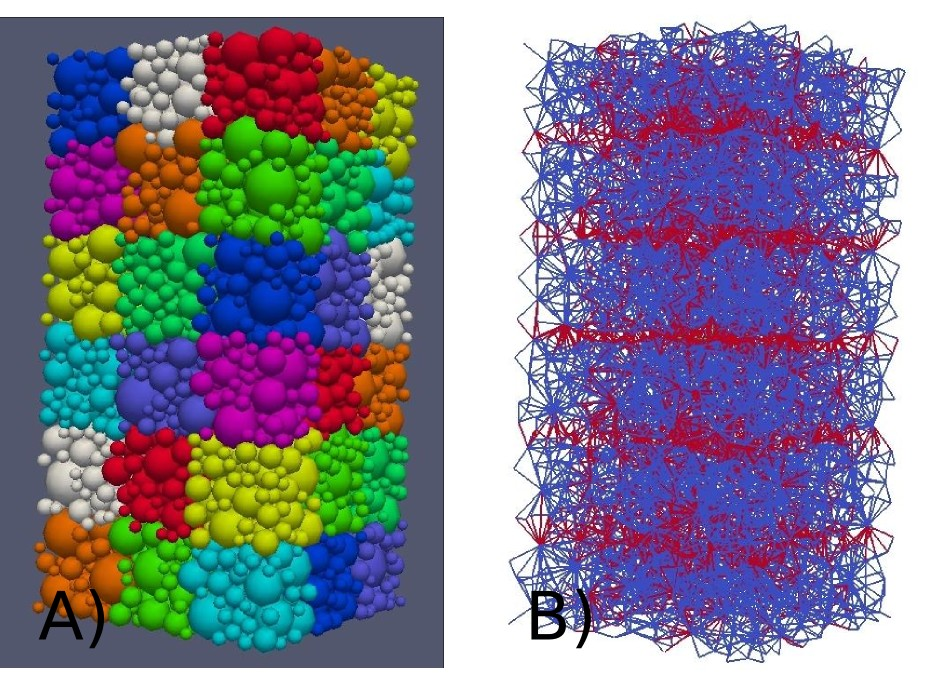
\includegraphics{cluster_box.jpg}}
\end{center}
\caption{Images (generated with Paraview) of a box with clustered particles generated by the script \texttt{cluster\_box.py} described in section \ref{sec:gengeo_clusterbox}. Panel A) shows the particles colored by particle tag. To enhance the visual contrast between neighboring clusters colors are set using particle tag modulo 10.  Panel B) shows the bonds in this model. Intra-cluster bonds (bond tag 0) are shown in blue and tags between clusters (bond tag 1) in red.} \label{fig:cluster_box}
\end{figure}
%% -----

\section{Lateral thinking: hierarchical packing for complex models}

\section{If nothing else helps - the \texttt{MeshVolume}}
\label{sec:mesh_volume}

For complicated geometries which can not be reasonably expressed as combination of simple volumes there is a way to fill any volume bounded by a closed, triangulated surface with particles. However, it should be noted that this can be computationally rather expensive, in particular that the computation time goes up roughly linear with the number of triangles forming the surface. On the other hand, it is usually faster than constructing the same volume from a set of convex polyhedra. Also, it should be noted that there is currently no facility to import any given mesh format into \texttt{GenGeo}. 

\section{What else is there?}
This section provides short descriptions of the remaining features of the \texttt{GenGeo} library. Features marked \textit{EXPERIMENTAL} may not be completely implemented and / or tested yet and therefore have bugs and limitations.   
 
\subsection{Volumes}
\subsubsection*{BoxWithJointSet}
\subsubsection*{ConvexPolyhedron}
\subsubsection*{SphereVol}
\subsubsection*{ClippedSphereVol}
\subsubsection*{CylinderVol}
\subsubsection*{CylinderWithJointSet}
\subsubsection*{DogBone}
\subsubsection*{EllipsoidVol \textit{EXPERIMENTAL}}
\subsubsection*{Constructive Solid Geometry (CSG) based volumes \textit{EXPERIMENTAL}}
\subsubsection{Objects}
\subsubsection{Tagging and Bonding}
\section*{What's Next?}
\newpage
\section{Additional ESyS-Particle resources and documentation}

\appendix
\chapter{Code-listings for tutorial examples}\label{code}
\section{ESyS-Particle scripts}
\subsection{\texttt{bingle.py}}\label{code:bingle}

\begin{verbatim}
#bingle.py: A simple two-particle collision simulation using
#           ESyS-Particle
#       Author: D. Weatherley
#       Date: 15 May 2007
#       Organisation: ESSCC, University of Queensland
#       (C) All rights reserved, 2007.
#
#
#import the appropriate ESyS-Particle modules:
from esys.lsm import *
from esys.lsm.util import Vec3, BoundingBox

#instantiate a simulation object
#and initialise the neighbour search algorithm:
sim = LsmMpi(numWorkerProcesses=1, mpiDimList=[1,1,1])
sim.initNeighbourSearch(
   particleType="NRotSphere",
   gridSpacing=2.5,
   verletDist=0.5
)

#specify the number of timesteps and timestep increment:
sim.setNumTimeSteps(10000)
sim.setTimeStepSize(0.001)

#specify the spatial domain for the simulation:
domain = BoundingBox(Vec3(-20,-20,-20), Vec3(20,20,20))
sim.setSpatialDomain(domain)

#add the first particle to the domain:
particle=NRotSphere(id=0, posn=Vec3(-5,5,-5), radius=1.0, mass=1.0)
particle.setLinearVelocity(Vec3(1.0,-1.0,1.0))
sim.createParticle(particle)

#add the second particle to the domain:
particle=NRotSphere(id=1, posn=Vec3(5,5,5), radius=1.5, mass=2.0)
particle.setLinearVelocity(Vec3(-1.0,-1.0,-1.0))
sim.createParticle(particle)

#specify the type of interactions between colliding particles:
sim.createInteractionGroup(
   NRotElasticPrms(
      name = "elastic_repulsion",
      normalK = 10000.0,
      scaling = True
   )
)

#Execute the simulation:
sim.run()
\end{verbatim}

\subsection{\texttt{bingle\_output.py}}\label{code:bingle_output}

\begin{verbatim}
#bingle_output.py: A two-particle collision simulation 
#                  with ASCII data output
#	Author: D. Weatherley
#	Date: 15 May 2007
#	Organisation: ESSCC, University of Queensland
#	(C) All rights reserved, 2007.
#
#


#provide forward compatibility for Python 2 interpreters
from __future__ import print_function

#import the appropriate ESyS-Particle modules:
from esys.lsm import *
from esys.lsm.util import Vec3, BoundingBox

#instantiate a simulation object 
#and initialise the neighbour search algorithm:
sim = LsmMpi(numWorkerProcesses=1, mpiDimList=[1,1,1])
sim.initNeighbourSearch(
   particleType="NRotSphere",
   gridSpacing=2.5,
   verletDist=0.5
)

#set the number of timesteps and timestep increment:
sim.setNumTimeSteps(10000)
sim.setTimeStepSize(0.001)

#specify the spatial domain for the simulation:
domain = BoundingBox(Vec3(-20,-20,-20), Vec3(20,20,20))
sim.setSpatialDomain(domain)

#add the first particle to the domain:
particle=NRotSphere(id=0, posn=Vec3(-5,5,-5), radius=1.0, mass=1.0)
particle.setLinearVelocity(Vec3(1.0,-1.0,1.0))
sim.createParticle(particle)

#add the second particle to the domain:
particle=NRotSphere(id=1, posn=Vec3(5,5,5), radius=1.5, mass=2.0)
particle.setLinearVelocity(Vec3(-1.0,-1.0,-1.0))
sim.createParticle(particle)

#specify the type of interactions between colliding particles:
sim.createInteractionGroup(
   NRotElasticPrms(
      name = "elastic_repulsion",
      normalK = 10000.0,
      scaling = True
   )
)

#compute the specified number of timesteps:
N_max = sim.getNumTimeSteps()
n=0
while (n < N_max):
   #compute a single timestep:
   sim.runTimeStep()

   # print the particle position to stdout every 100 timesteps:
   if (n%100==0):
      particles = sim.getParticleList()
      p1 = particles[0].getPosn()
      p2 = particles[1].getPosn()
      print(n,p1,p2)

   # update the total number of timesteps computed (n):
   n += 1

#Exit the simulation.
sim.exit()
\end{verbatim}

\subsection{\texttt{bingle\_chk.py}}\label{code:bingle_chk}

\begin{verbatim}
#bingle_chk.py: A simple two-particle collision simulation 
#               with data output via a CheckPointer
#	Author: D. Weatherley
#	Date: 15 May 2007
#	Organisation: ESSCC, University of Queensland
#	(C) All rights reserved, 2007.
#
#
#import the appropriate ESyS-Particle modules:
from esys.lsm import *
from esys.lsm.util import Vec3, BoundingBox

#instantiate a simulation object 
#and initialise the neighbour search algorithm:
sim = LsmMpi(numWorkerProcesses=1, mpiDimList=[1,1,1])
sim.initNeighbourSearch(
   particleType="NRotSphere",
   gridSpacing=2.5,
   verletDist=0.5
)

#specify the number of timesteps and timestep increment 
sim.setNumTimeSteps(10000)
sim.setTimeStepSize(0.001)

#specify the spatial domain for the simulation:
domain = BoundingBox(Vec3(-20,-20,-20), Vec3(20,20,20))
sim.setSpatialDomain(domain)

#add the first particle to the domain:
particle=NRotSphere(id=0, posn=Vec3(-5,5,-5), radius=1.0, mass=1.0)
particle.setLinearVelocity(Vec3(1.0,-1.0,1.0))
sim.createParticle(particle)

#add the second particle to the domain:
particle=NRotSphere(id=1, posn=Vec3(5,5,5), radius=1.5, mass=2.0)
particle.setLinearVelocity(Vec3(-1.0,-1.0,-1.0))
sim.createParticle(particle)

#specify the type of interactions between colliding particles:
sim.createInteractionGroup(
   NRotElasticPrms(
      name = "elastic_repulsion",
      normalK = 10000.0,
      scaling = True
   )
)

#add a CheckPointer to save simulation data at regular intervals:
sim.createCheckPointer (
   CheckPointPrms (
      fileNamePrefix = "bingle_data",
      beginTimeStep = 0,
      endTimeStep = 10000,
      timeStepIncr = 100
   )
)

#Execute the simulation
sim.run()
\end{verbatim}


\subsection{\texttt{bingle\_vis.py}}\label{code:bingle_vis}

\begin{verbatim}
#bingle_vis.py: A two-particle collision simulation 
#               with visualisation using povray
#	Author: D. Weatherley
#	Date: 15 May 2007
#	Organisation: ESSCC, University of Queensland
#	(C) All rights reserved, 2007.
#
#
#import the appropriate ESyS-Particle modules:
from esys.lsm import *
from esys.lsm.util import Vec3, BoundingBox
from esys.lsm.vis import povray

def snapshot(particles=None, index=0):
   pkg = povray
   scene = pkg.Scene()
   for pp in particles: 
      povsphere = pkg.Sphere(pp.getPosn(), pp.getRadius())
      povsphere.apply(pkg.Colors.Red)
      scene.add(povsphere)

   camera = scene.getCamera()
   camera.setLookAt(Vec3(0,0,0))
   camera.setPosn(Vec3(0,0,20))
   camera.setZoom(0.1)

   scene.render(
      offScreen=True,
      interactive=False,
      fileName="snap_{0:04d}.png".format(index),
      size=[800,600]
   )
   return

#instantiate a simulation object 
#and initialise the neighbour search algorithm:
sim = LsmMpi(numWorkerProcesses=1, mpiDimList=[1,1,1])
sim.initNeighbourSearch(
   particleType="NRotSphere",
   gridSpacing=2.5,
   verletDist=0.5
)

#set the number of timesteps and timestep increment:
sim.setNumTimeSteps(10000)
sim.setTimeStepSize(0.001)

#specify the spatial domain for the simulation:
domain = BoundingBox(Vec3(-20,-20,-20), Vec3(20,20,20))
sim.setSpatialDomain(domain)

#add the first particle to the domain:
particle=NRotSphere(id=0, posn=Vec3(-5,5,-5), radius=1.0, mass=1.0)
particle.setLinearVelocity(Vec3(1.0,-1.0,1.0))
sim.createParticle(particle)

#add the second particle to the domain:
particle=NRotSphere(id=1, posn=Vec3(5,5,5), radius=1.5, mass=2.0)
particle.setLinearVelocity(Vec3(-1.0,-1.0,-1.0))
sim.createParticle(particle)

#specify the type of interactions between colliding particles:
sim.createInteractionGroup(
   NRotElasticPrms(
      name = "elastic_repulsion",
      normalK = 10000.0,
      scaling = True
   )
)

#compute the specified number of timesteps:
N_max = sim.getNumTimeSteps()
n=0
while (n < N_max):
   #compute a single timestep:
   sim.runTimeStep()

   # Take a snapshot of the simulation every 100 timesteps:
   if (n%100==0):
      particles = sim.getParticleList()
      snapshot(particles=particles, index=n)

   # update the total number of timesteps computed (n):
   n += 1

#Exit the simulation.
sim.exit()
\end{verbatim}

\subsection{\texttt{POVsnaps.py}}\label{code:POVsnaps}

\begin{verbatim}
#POVsnaps.py: Implements an ESyS-Particle runnable for storing 
#             snapshots of particle simulations rendered using POVray
#	Author: D. Weatherley
#	Date:	17 May 2007
#	Organisation: ESSCC, University of Queensland
#	(C) All Rights Reserved, 2007.

from esys.lsm import *
from esys.lsm.util import Vec3, BoundingBox
from esys.lsm.vis import povray

class POVsnaps (Runnable):
   def __init__(self, sim, interval):
      Runnable.__init__(self)
      self.sim = sim
      self.interval = interval
      self.count = 0
      self.configure()

   def configure(
      self, 
      lookAt=Vec3(0,0,0), 
      camPosn=Vec3(0,0,20), 
      zoomFactor=0.1, 
      imageSize=[800,600]):

      self.lookAt=lookAt
      self.camPosn=camPosn
      self.zoomFactor=zoomFactor
      self.imageSize=imageSize

   def run(self):
      if ((self.sim.getTimeStep() % self.interval) == 0):
         self.snapshot()
         self.count += 1

   def snapshot(self):
      pkg = povray
      Scene = pkg.Scene()
      plist = self.sim.getParticleList()

      for pp in plist:
         povsphere = pkg.Sphere(pp.getPosn(), pp.getRadius())
         povsphere.apply(pkg.Colors.Red)
         Scene.add(povsphere)

      camera = Scene.getCamera()
      camera.setLookAt(self.lookAt)
      camera.setPosn(self.camPosn)
      camera.setZoom(self.zoomFactor)

      fname = "snap_{0:04d}.png".format(self.count)
      Scene.render(
         offScreen=True, 
         interactive=False, 
         fileName=fname, 
         size=self.imageSize
      )
\end{verbatim}


\subsection{\texttt{bingle\_Runnable.py}}\label{code:bingle_Runnable}

\begin{verbatim}
#bingle_Runnable.py: A two-particle collision simulation 
#                    with visualisation via a Runnable 
#	Author: D. Weatherley
#	Date: 17 May 2007
#	Organisation: ESSCC, University of Queensland
#	(C) All rights reserved, 2007.
#
#
#import the appropriate ESyS-Particle modules:
from esys.lsm import *
from esys.lsm.util import Vec3, BoundingBox
from POVsnaps import POVsnaps

#instantiate a simulation object 
#and initialise the neighbour search algorithm:
sim = LsmMpi(numWorkerProcesses=1, mpiDimList=[1,1,1])
sim.initNeighbourSearch(
   particleType="NRotSphere",
   gridSpacing=2.5,
   verletDist=0.5
)

#set the number of timesteps and timestep increment:
sim.setNumTimeSteps(10000)
sim.setTimeStepSize(0.001)

#specify the spatial domain for the simulation:
domain = BoundingBox(Vec3(-20,-20,-20), Vec3(20,20,20))
sim.setSpatialDomain(domain)

#add the first particle to the domain:
particle=NRotSphere(id=0, posn=Vec3(-5,5,-5), radius=1.0, mass=1.0)
particle.setLinearVelocity(Vec3(1.0,-1.0,1.0))
sim.createParticle(particle)

#add the second particle to the domain:
particle=NRotSphere(id=1, posn=Vec3(5,5,5), radius=1.5, mass=2.0)
particle.setLinearVelocity(Vec3(-1.0,-1.0,-1.0))
sim.createParticle(particle)

#specify the type of interactions between colliding particles:
sim.createInteractionGroup(
   NRotElasticPrms(
      name = "elastic_repulsion",
      normalK = 10000.0,
      scaling = True
   )
)

#add a POVsnaps Runnable for taking images 
#of the particles every 100 timesteps:
povcam = POVsnaps(sim=sim, interval=100)
sim.addPostTimeStepRunnable(povcam)

#execute the simulation:
sim.run()
\end{verbatim}


\subsection{\texttt{gravity.py}}\label{code:gravity}

\begin{verbatim}
#gravity.py: A simple bouncing ball simulation using ESyS-Particle
#	Author: D. Weatherley
#	Date: 15 May 2007
#	Organisation: ESSCC, University of Queensland
#	(C) All rights reserved, 2007.
#
#
#import the appropriate ESyS-Particle modules:
from esys.lsm import *
from esys.lsm.util import Vec3, BoundingBox
from POVsnaps import POVsnaps

#instantiate a simulation object 
#and initialise the neighbour search algorithm:
sim = LsmMpi(numWorkerProcesses=1, mpiDimList=[1,1,1])
sim.initNeighbourSearch(
   particleType="NRotSphere",
   gridSpacing=2.5,
   verletDist=0.5
)

#set the number of timesteps and timestep increment:
sim.setNumTimeSteps(20000)
sim.setTimeStepSize(0.001)

#specify the spatial domain for the simulation:
domain = BoundingBox(Vec3(-20,-20,-20), Vec3(20,20,20))
sim.setSpatialDomain(domain)

#add a particle to the domain:
particle=NRotSphere(id=0, posn=Vec3(0,5,0), radius=1.75, mass=1.8)
particle.setLinearVelocity(Vec3(1.0,10.0,1.0))
sim.createParticle(particle)

#initialise gravity in the domain:
sim.createInteractionGroup(
   GravityPrms(name="earth-gravity", acceleration=Vec3(0,-9.81,0))
)

#add a horizontal wall to act as a floor on which to bounce particles:
sim.createWall(
   name="floor",
   posn=Vec3(0,-10,0),
   normal=Vec3(0,1,0)
)

#specify the type of interactions between wall and particles:
sim.createInteractionGroup(
   NRotElasticWallPrms(
      name = "elasticWall",
      wallName = "floor",
      normalK = 10000.0
   )
)

#add local viscosity to simulate air resistance:
sim.createInteractionGroup(
    LinDampingPrms(
        name="linDamping",
        viscosity=0.1,
        maxIterations=100
    )
)

#add a POVsnaps Runnable:
povcam = POVsnaps(sim=sim, interval=100)
povcam.configure()
sim.addPostTimeStepRunnable(povcam)

#execute the simulation
sim.run()
\end{verbatim}


\subsection{\texttt{gravity\_cube.py}}\label{code:gravity_cube}

\begin{verbatim}
#gravity_cube.py: A bouncing cube simulation using ESyS-Particle
#       Author: D. Weatherley
#       Date: 15 May 2007
#       Organisation: ESSCC, University of Queensland
#       (C) All rights reserved, 2007.
#
#
#import the division module for compatibility between Python 2 and Python 3
from __future__ import division
#import the appropriate ESyS-Particle modules:
from esys.lsm import *
from esys.lsm.util import Vec3, BoundingBox
from esys.lsm.geometry import CubicBlock,ConnectionFinder
from POVsnaps import POVsnaps

#instantiate a simulation object
#and initialise the neighbour search algorithm:
sim = LsmMpi(numWorkerProcesses=1, mpiDimList=[1,1,1])
sim.initNeighbourSearch(
   particleType="NRotSphere",
   gridSpacing=2.5,
   verletDist=0.5
)

#set the number of timesteps and timestep increment:
sim.setNumTimeSteps(10000)
sim.setTimeStepSize(0.001)

#specify the spatial domain for the simulation:
domain = BoundingBox(Vec3(-20,-20,-20), Vec3(20,20,20))
sim.setSpatialDomain(domain)

#add a cube of particles to the domain:
cube = CubicBlock(dimCount=[6,6,6], radius=0.5)
cube.rotate(axis=Vec3(0,0,3.141592654/6.0),axisPt=Vec3(0,0,0))
sim.createParticles(cube)

#create bonds between particles separated by less than the specified
#maxDist:
sim.createConnections(
   ConnectionFinder(
      maxDist = 0.005,
      bondTag = 1,
      pList = cube
   )
)

#specify bonded elastic interactions between bonded particles:
bondGrp = sim.createInteractionGroup(
   NRotBondPrms(
      name = "sphereBonds",
      normalK = 10000.0,
      breakDistance = 50.0,
      tag = 1,
      scaling = True
   )
)

#initialise gravity in the domain:
sim.createInteractionGroup(
   GravityPrms(name="earth-gravity", acceleration=Vec3(0,-9.81,0))
)

#add a horizontal wall to act as a floor to bounce particle off:
sim.createWall(
   name="floor",
   posn=Vec3(0,-10,0),
   normal=Vec3(0,1,0)
)

#specify the type of interactions between wall and particles:
sim.createInteractionGroup(
   NRotElasticWallPrms(
      name = "elasticWall",
      wallName = "floor",
      normalK = 10000.0
   )
)

#add local viscosity to simulate air resistance:
sim.createInteractionGroup(
    LinDampingPrms(
        name="linDamping",
        viscosity=0.1,
        maxIterations=100
    )
)

#add a POVsnaps Runnable:
povcam = POVsnaps(sim=sim, interval=100)
povcam.configure(lookAt=Vec3(0,0,0), camPosn=Vec3(14,0,14))
sim.addPostTimeStepRunnable(povcam)

#execute the simulation
sim.run()
\end{verbatim}


\subsection{\texttt{slope\_fail.py}}\label{code:slope_fail}
\begin{verbatim}
#slope_fail.py: A slope failure simulation using ESyS-Particle
#       Author: D. Weatherley
#       Date: 23 December 2008
#       Organisation: ESSCC, University of Queensland
#       (C) All rights reserved, 2008.
#
#
#import the appropriate ESyS-Particle modules:
from esys.lsm import *
from esys.lsm.util import *
from esys.lsm.geometry import *

#instantiate a simulation object 
#and initialise the neighbour search algorithm:
sim = LsmMpi (numWorkerProcesses = 1, mpiDimList = [1,1,1])
sim.initNeighbourSearch (
   particleType = "NRotSphere",
   gridSpacing = 2.5000,
   verletDist = 0.1000
)

#specify the number of timesteps and the timestep increment:
sim.setNumTimeSteps (50000)
sim.setTimeStepSize (1.0000e-04)

#specify the spatial domain for the simulation:
domain = BoundingBox(Vec3(-20,-20,-20), Vec3(20,20,20))
sim.setSpatialDomain(domain)

#construct a block of particles with radii in range [0.2,0.5]:
geoRandomBlock = RandomBoxPacker (
   minRadius = 0.2000,
   maxRadius = 0.5000,
   cubicPackRadius = 2.2000,
   maxInsertFails = 1000,
   bBox = BoundingBox(
      Vec3(-5.0000, 0.0000,-5.0000),
      Vec3(5.0000, 10.0000, 5.0000)
   ),
   circDimList = [False, False, False],
   tolerance = 1.0000e-05
)
geoRandomBlock.generate()
geoRandomBlock_particles = geoRandomBlock.getSimpleSphereCollection()

#add the particle assembly to the simulation object:
sim.createParticles(geoRandomBlock_particles)

#add a wall as a floor for the model:
sim.createWall (
   name = "floor",
   posn = Vec3(0.0000, 0.0000, 0.0000),
   normal = Vec3(0.0000, 1.0000, 0.0000)
)

#specify that particles undergo unbonded elastic repulsion:
sim.createInteractionGroup (
   NRotElasticPrms (
      name = "repulsion",
      normalK = 1.0000e+03,
      scaling = True
   )
)

#specify that particles undergo elastic repulsion from the floor:
sim.createInteractionGroup (
   NRotElasticWallPrms (
      name = "wall_repell",
      wallName = "floor",
      normalK = 1.0000e+04
   )
)

#specify the direction and magnitude of gravity:
sim.createInteractionGroup (
   GravityPrms (
      name = "gravity",
      acceleration = Vec3(0.0000, -9.8100, 0.0000)
   )
)

#add viscosity to damp particle oscillations:
sim.createInteractionGroup (
   LinDampingPrms (
      name = "viscosity",
      viscosity = 0.1000,
      maxIterations = 100
   )
)

#add a CheckPointer to store simulation data:
sim.createCheckPointer (
   CheckPointPrms (
      fileNamePrefix = "slope_data",
      beginTimeStep = 0,
      endTimeStep = 50000,
      timeStepIncr = 1000
   )
)

#execute the simulation:
sim.run()
\end{verbatim}


\subsection{\texttt{slope\_friction.py}}\label{code:slope_friction}
\begin{verbatim}
#slope_friction.py: A slope failure simulation with friction using
#                   ESyS-Particle
#       Author: D. Weatherley
#       Date: 23 December 2008
#       Organisation: ESSCC, University of Queensland
#       (C) All rights reserved, 2008.
#
#
#import the appropriate ESyS-Particle modules:
from esys.lsm import *
from esys.lsm.util import *
from esys.lsm.geometry import *

#instantiate a simulation object 
#and initialise the neighbour search algorithm:
sim = LsmMpi (numWorkerProcesses = 1, mpiDimList = [1,1,1])
sim.initNeighbourSearch (
   particleType = "NRotSphere",
   gridSpacing = 2.5000,
   verletDist = 0.1000
)

#specify the number of timesteps and the timestep increment:
sim.setNumTimeSteps (50000)
sim.setTimeStepSize (1.0000e-04)

#specify the spatial domain for the simulation:
domain = BoundingBox(Vec3(-20,-20,-20), Vec3(20,20,20))
sim.setSpatialDomain(domain)

#construct a block of particles with radii in range [0.2,0.5]:
geoRandomBlock = RandomBoxPacker (
   minRadius = 0.2000,
   maxRadius = 0.5000,
   cubicPackRadius = 2.2000,
   maxInsertFails = 1000,
   bBox = BoundingBox(
      Vec3(-5.0000, 0.0000,-5.0000),
      Vec3(5.0000, 10.0000, 5.0000)
   ),
   circDimList = [False, False, False],
   tolerance = 1.0000e-05
)
geoRandomBlock.generate()
geoRandomBlock_particles = geoRandomBlock.getSimpleSphereCollection()

#add the particle assembly to the simulation object:
sim.createParticles(geoRandomBlock_particles)

#add a wall as a floor for the model:
sim.createWall (
   name = "floor",
   posn = Vec3(0.0000, 0.0000, 0.0000),
   normal = Vec3(0.0000, 1.0000, 0.0000)
)

#specify that particles undergo frictional interactions:
sim.createInteractionGroup (
   NRotFrictionPrms (
      name = "friction",
      normalK = 1000.0,
      dynamicMu = 0.6,
      shearK = 100.0,
      scaling = True
   )
)

#specify that particles undergo elastic repulsion from the floor:
sim.createInteractionGroup (
   NRotElasticWallPrms (
      name = "wall_repell",
      wallName = "floor",
      normalK = 1.0000e+04
   )
)

#specify the direction and magnitude of gravity:
sim.createInteractionGroup (
   GravityPrms (
      name = "gravity",
      acceleration = Vec3(0.0000, -9.8100, 0.0000)
   )
)

#add viscosity to damp particle oscillations:
sim.createInteractionGroup (
   LinDampingPrms (
      name = "viscosity",
      viscosity = 0.1000,
      maxIterations = 100
   )
)

#add a CheckPointer to store simulation data:
sim.createCheckPointer (
   CheckPointPrms (
      fileNamePrefix = "slope_data",
      beginTimeStep = 0,
      endTimeStep = 50000,
      timeStepIncr = 1000
   )
)

#execute the simulation:
sim.run()
\end{verbatim}


\subsection{\texttt{slope\_friction\_floor.py}}\label{code:slope_friction_floor}
\begin{verbatim}
#slope_friction_floor.py: A slope failure simulation with friction 
#                         and a bumpy floor using ESyS-Particle
#       Author: D. Weatherley
#       Date: 23 December 2008
#       Organisation: ESSCC, University of Queensland
#       (C) All rights reserved, 2008.
#
#
#import the appropriate ESyS-Particle modules:
from esys.lsm import *
from esys.lsm.util import *
from esys.lsm.geometry import *

#instantiate a simulation object 
#and initialise the neighbour search algorithm:
sim = LsmMpi (numWorkerProcesses = 1, mpiDimList = [1,1,1])
sim.initNeighbourSearch (
   particleType = "NRotSphere",
   gridSpacing = 2.5000,
   verletDist = 0.1000
)

#specify the number of timesteps and the timestep increment:
sim.setNumTimeSteps (100000)
sim.setTimeStepSize (1.0000e-04)

#specify the spatial domain for the simulation:
domain = BoundingBox(Vec3(-20,-20,-20), Vec3(20,20,20))
sim.setSpatialDomain(domain)

#construct a block of particles with radii in range [0.2,0.5]:
geoRandomBlock = RandomBoxPacker (
   minRadius = 0.2000,
   maxRadius = 0.5000,
   cubicPackRadius = 2.2000,
   maxInsertFails = 1000,
   bBox = BoundingBox(
      Vec3(-5.0000, 0.0000,-5.0000),
      Vec3(5.0000, 10.0000, 5.0000)
   ),
   circDimList = [False, False, False],
   tolerance = 1.0000e-05
)
geoRandomBlock.generate()
geoRandomBlock_particles = geoRandomBlock.getSimpleSphereCollection()

#add particles to simulation one at a time, 
#tagging those nearest the floor:
for pp in geoRandomBlock_particles:
   centre = pp.getPosn()
   radius = pp.getRadius()
   Y = centre[1]
   if (Y < 1.1*radius):
      pp.setTag(12321)		# tag particles nearest to the floor
   sim.createParticle(pp)	# add the particle to the simulation object

#add a wall as a floor for the model:
sim.createWall (
   name = "floor",
   posn = Vec3(0.0000, 0.0000, 0.0000),
   normal = Vec3(0.0000, 1.0000, 0.0000)
)

#specify that particles undergo frictional interactions:
sim.createInteractionGroup (
   NRotFrictionPrms (
      name = "friction",
      normalK = 1000.0,
      dynamicMu = 0.6,
      shearK = 100.0,
      scaling = True
   )
)

#specify that tagged particles undergo 
#bonded elastic interactions with floor:
sim.createInteractionGroup (
   NRotBondedWallPrms (
      name = "floor_bonds",
      wallName = "floor",
      normalK = 10000.0,
      particleTag = 12321
   )
)

#specify the direction and magnitude of gravity:
sim.createInteractionGroup (
   GravityPrms (
      name = "gravity",
      acceleration = Vec3(0.0000, -9.8100, 0.0000)
   )
)

#add viscosity to damp particle oscillations:
sim.createInteractionGroup (
   LinDampingPrms (
      name = "viscosity",
      viscosity = 0.1000,
      maxIterations = 100
   )
)

#add a CheckPointer to store simulation data:
sim.createCheckPointer (
   CheckPointPrms (
      fileNamePrefix = "slope_data",
      beginTimeStep = 0,
      endTimeStep = 100000,
      timeStepIncr = 1000
   )
)

#execute the simulation:
sim.run()
\end{verbatim}


\subsection{\texttt{slope\_friction\_walls.py}}\label{code:slope_friction_walls}
\begin{verbatim}
#slope_friction_walls.py: A slope failure simulation using quarter 
#                         symmetry and a bumpy floor using ESyS-Particle
#       Author: D. Weatherley
#       Date: 23 December 2008
#       Organisation: ESSCC, University of Queensland
#       (C) All rights reserved, 2008.
#
#
#import the appropriate ESyS-Particle modules:
from esys.lsm import *
from esys.lsm.util import *
from esys.lsm.geometry import *

#instantiate a simulation object and 
#initialise the neighbour search algorithm:
sim = LsmMpi (numWorkerProcesses = 1, mpiDimList = [1,1,1])
sim.initNeighbourSearch (
   particleType = "NRotSphere",
   gridSpacing = 2.5000,
   verletDist = 0.1000
)

#specify the number of timesteps and the timestep increment:
sim.setNumTimeSteps (100000)
sim.setTimeStepSize (1.0000e-04)

#specify the spatial domain for the simulation:
domain = BoundingBox(Vec3(-20,-20,-20), Vec3(20,20,20))
sim.setSpatialDomain(domain)

#construct a block of particles with radii in range [0.2,0.5]:
geoRandomBlock = RandomBoxPacker (
   minRadius = 0.2000,
   maxRadius = 0.5000,
   cubicPackRadius = 2.2000,
   maxInsertFails = 1000,
   bBox = BoundingBox(
      Vec3(-5.0000, 0.0000,-5.0000),
      Vec3(5.0000, 10.0000, 5.0000)
   ),
   circDimList = [False, False, False],
   tolerance = 1.0000e-05
)
geoRandomBlock.generate()
geoRandomBlock_particles = geoRandomBlock.getSimpleSphereCollection()

#add particles to simulation one at a time, 
#tagging those nearest the floor
for pp in geoRandomBlock_particles:
   centre = pp.getPosn()
   radius = pp.getRadius()
   Y = centre[1]
   if (Y < 1.1*radius):
      pp.setTag(12321)		# tag particles nearest to the floor
   sim.createParticle(pp)	# add the particle to the simulation object

#add a wall as a floor for the model:
sim.createWall (
   name = "floor",
   posn = Vec3(0.0000, 0.0000, 0.0000),
   normal = Vec3(0.0000, 1.0000, 0.0000)
)

#add a left side wall to the model:
sim.createWall (
   name = "left_wall",
   posn = Vec3(-5.0000, 0.0000, 0.0000),
   normal = Vec3(1.0000, 0.0000, 0.0000)
)

#add a back wall to the model:
sim.createWall (
   name = "back_wall",
   posn = Vec3(0.0000, 0.0000, -5.0000),
   normal = Vec3(0.0000, 0.0000, 1.0000)
)

#specify that particles undergo frictional interactions:
sim.createInteractionGroup (
   NRotFrictionPrms (
      name = "friction",
      normalK = 1000.0,
      dynamicMu = 0.6,
      shearK = 100.0,
      scaling = True
   )
)

#specify that particles with tag 12321 undergo 
#bonded elastic interactions with floor:
sim.createInteractionGroup (
   NRotBondedWallPrms (
      name = "floor_bonds",
      wallName = "floor",
      normalK = 10000.0,
      particleTag = 12321
   )
)

#specify that particles undergo elastic repulsion
#from the left side wall:
sim.createInteractionGroup (
   NRotElasticWallPrms (
      name = "lw_repel",
      wallName = "left_wall",
      normalK = 1.0000e+04
   )
)

#specify that particles undergo elastic repulsion
#from the back wall:
sim.createInteractionGroup (
   NRotElasticWallPrms (
      name = "bw_repel",
      wallName = "back_wall",
      normalK = 1.0000e+04
   )
)

#specify the direction and magnitude of gravity:
sim.createInteractionGroup (
   GravityPrms (
      name = "gravity",
      acceleration = Vec3(0.0000, -9.8100, 0.0000)
   )
)

#add viscosity to damp particle oscillations:
sim.createInteractionGroup (
   LinDampingPrms (
      name = "viscosity",
      viscosity = 0.1000,
      maxIterations = 100
   )
)

#add a CheckPointer to store simulation data:
sim.createCheckPointer (
   CheckPointPrms (
      fileNamePrefix = "slope_data",
      beginTimeStep = 0,
      endTimeStep = 100000,
      timeStepIncr = 1000
   )
)

#execute the simulation:
sim.run()
\end{verbatim}


\subsection{\texttt{floorMesh.msh}}\label{code:floorMesh}
\begin{verbatim}
Triangle
3D-Nodes 6
 0  0 0  -5.0  0.0   0.0
 1  1 0  -5.0  0.0   5.0
 2  2 0   0.0  0.0  -5.0
 3  3 0   0.0  0.0   0.0
 4  4 0   5.0  0.0  -5.0
 5  5 0   5.0  0.0   5.0

Tri3 4
 0  0  0  3  1
 1  0  1  3  5
 2  0  5  3  4
 3  0  3  2  4
\end{verbatim}


\subsection{\texttt{hopper\_flow.py}}\label{code:hopper_flow}
\begin{verbatim}
#hopper_flow.py: A hopper flow simulation with mesh walls using
#                ESyS-Particle
#       Author: W. Hancock
#       Date: 10 July 2009
#       Organisation: ESSCC, University of Queensland
#       (C) All rights reserved, 2009.
#
#
#import the appropriate ESyS-Particle modules:
from esys.lsm import *
from esys.lsm.util import *
from esys.lsm.geometry import *

#instantiate a simulation object and
#initialise the neighbour search algorithm:
sim = LsmMpi (numWorkerProcesses = 1, mpiDimList = [1,1,1])
sim.initNeighbourSearch (
   particleType = "NRotSphere",
   gridSpacing = 2.5000,
   verletDist = 0.1000
)

#specify the number of timesteps and the timestep increment:
sim.setNumTimeSteps (100000)
sim.setTimeStepSize (1.0000e-04)

#specify the spatial domain for the simulation:
domain = BoundingBox(Vec3(-20,-20,-20), Vec3(20,20,20))
sim.setSpatialDomain(domain)

#construct a block of particles with radii in range [0.2,0.5]:
geoRandomBlock = RandomBoxPacker (
   minRadius = 0.2000,
   maxRadius = 0.5000,
   cubicPackRadius = 2.2000,
   maxInsertFails = 1000,
   bBox = BoundingBox(
      Vec3(-5.0000, 0.0000,-5.0000),
      Vec3(5.0000, 10.0000, 5.0000)
   ),
   circDimList = [False, False, False],
   tolerance = 1.0000e-05
)
geoRandomBlock.generate()
geoRandomBlock_particles = geoRandomBlock.getSimpleSphereCollection()

#add particles to simulation one at a time,
#tagging those in layers of 2m
for pp in geoRandomBlock_particles:
   centre = pp.getPosn()
   Y = centre[1]
   if (int(Y%4) < 2):
      pp.setTag(1) # layer 1
   else:
      pp.setTag(2) # layer 2
   sim.createParticle(pp) # add the particle to the simulation object

#add a wall as a floor for the model:
sim.readMesh(
   fileName = "floorMesh.msh",
   meshName = "floor_mesh_wall"
)

#add a left side wall to the model:
sim.createWall (
   name = "left_wall",
   posn = Vec3(-5.0000, 0.0000, 0.0000),
   normal = Vec3(1.0000, 0.0000, 0.0000)
)

#add a right side wall to the model:
sim.createWall (
   name = "right_wall",
   posn = Vec3(5.0000, 0.0000, 0.0000),
   normal = Vec3(-1.0000, 0.0000, 0.0000)
)

#add a back wall to the model:
sim.createWall (
   name = "back_wall",
   posn = Vec3(0.0000, 0.0000, -5.0000),
   normal = Vec3(0.0000, 0.0000, 1.0000)
)

#add a front wall to the model:
sim.createWall (
   name = "front_wall",
   posn = Vec3(0.0000, 0.0000, 5.0000),
   normal = Vec3(0.0000, 0.0000, -1.0000)
)

#specify that particles undergo frictional interactions:
sim.createInteractionGroup (
   NRotFrictionPrms (
      name = "friction",
      normalK = 1000.0,
      dynamicMu = 0.6,
      shearK = 100.0,
      scaling = True
   )
)

#specify that particles undergo elastic repulsion
#with the floor mesh wall:
sim.createInteractionGroup (
   NRotElasticTriMeshPrms (
      name = "floorWall_repell",
      meshName = "floor_mesh_wall",
      normalK = 1.0000e+04
   )
)

#specify that particles undergo elastic repulsion
#from the left side wall:
sim.createInteractionGroup (
   NRotElasticWallPrms (
      name = "lw_repell",
      wallName = "left_wall",
      normalK = 1.0000e+04
   )
)
#specify that particles undergo elastic repulsion
#from the right side wall:
sim.createInteractionGroup (
   NRotElasticWallPrms (
      name = "rw_repell",
      wallName = "right_wall",
      normalK = 1.0000e+04
   )
)

#specify that particles undergo elastic repulsion
#from the back wall:
sim.createInteractionGroup (
   NRotElasticWallPrms (
      name = "bw_repell",
      wallName = "back_wall",
      normalK = 1.0000e+04
   )
)

#specify that particles undergo elastic repulsion
#from the front wall:
sim.createInteractionGroup (
   NRotElasticWallPrms (
      name = "fw_repell",
      wallName = "front_wall",
      normalK = 1.0000e+04
   )
)

#specify the direction and magnitude of gravity:
sim.createInteractionGroup (
   GravityPrms (
      name = "gravity",
      acceleration = Vec3(0.0000, -9.8100, 0.0000)
   )
)

#add viscosity to damp particle oscillations:
sim.createInteractionGroup (
   LinDampingPrms (
      name = "viscosity",
      viscosity = 0.1000,
      maxIterations = 100
   )
)

#add a CheckPointer to store simulation data:
sim.createCheckPointer (
   CheckPointPrms (
      fileNamePrefix = "flow_data",
      beginTimeStep = 0,
      endTimeStep = 100000,
      timeStepIncr = 1000
   )
)

#execute the simulation:
sim.run()
\end{verbatim}


\subsection{\texttt{rot\_compress.py}}\label{code:rot_compress}
\begin{verbatim}
#rot_compress.py: A uniaxial compression simulation using ESyS-Particle
#       Author: D. Weatherley
#       Date: 27 December 2008
#       Organisation: ESSCC, University of Queensland
#       (C) All rights reserved, 2008.
#
#
#import the appropriate ESyS-Particle modules:
from esys.lsm import *
from esys.lsm.util import *
from esys.lsm.geometry import *
from WallLoader import WallLoaderRunnable

#instantiate a simulation object: 
sim = LsmMpi (numWorkerProcesses = 1, mpiDimList = [1,1,1])

#initialise the neighbour search algorithm:
sim.initNeighbourSearch (
   particleType = "RotSphere",
   gridSpacing = 5.0000,
   verletDist = 0.08000
)

#set the number of timesteps and timestep increment:
sim.setNumTimeSteps (250000)
sim.setTimeStepSize (1.0000e-06) 

#specify the spatial domain for the simulation
domain = BoundingBox(Vec3(-20,-20,-20), Vec3(20,20,20))
sim.setSpatialDomain (domain)

#create a prism of spherical particles:
geoRandomBlock = RandomBoxPacker (
   minRadius = 0.400,
   maxRadius = 2.0000,
   cubicPackRadius = 2.2000,
   maxInsertFails = 5000,
   bBox = BoundingBox(
      Vec3(-5.0000, 0.0000,-5.0000),
      Vec3(5.0000, 20.0000, 5.0000)
   ),
   circDimList = [False, False, False],
   tolerance = 1.0000e-05
)
geoRandomBlock.generate()
geoRandomBlock_particles = geoRandomBlock.getSimpleSphereCollection()

#add the particles to the simulation object:
sim.createParticles(geoRandomBlock_particles)

#bond particles together with bondTag = 1:
sim.createConnections(
   ConnectionFinder(
      maxDist = 0.005,
      bondTag = 1,
      pList = geoRandomBlock_particles
   )
)

#create a wall at the bottom of the model:
sim.createWall (
   name = "bottom_wall",
   posn = Vec3(0.0000, 0.0000, 0.0000),
   normal = Vec3(0.0000, 1.0000, 0.0000)
)

#create a wall at the top of the model:
sim.createWall (
   name = "top_wall",
   posn = Vec3(0.0000, 20.0000, 0.0000),
   normal = Vec3(0.0000, -1.0000, 0.0000)
)

#create rotational elastic-brittle bonds between particles:
pp_bonds = sim.createInteractionGroup (
   BrittleBeamPrms(
      name="pp_bonds",
      youngsModulus=100000.0,
      poissonsRatio=0.25,
      cohesion=100.0,
      tanAngle=1.0,
      tag=1
   )
)

#initialise frictional interactions for unbonded particles:
sim.createInteractionGroup (
   FrictionPrms(
      name="friction",
      youngsModulus=100000.0,
      poissonsRatio=0.25,
      dynamicMu=0.4,
      staticMu=0.6
   ) 
)

#create an exclusion between bonded and frictional interactions:
sim.createExclusion (
   interactionName1 = "pp_bonds",
   interactionName2 = "friction"
)

#specify elastic repulsion from the bottom wall:
sim.createInteractionGroup (
   NRotElasticWallPrms (
      name = "bottom_wall_repel",
      wallName = "bottom_wall",
      normalK = 100000.0
   )
)

#specify elastic repulsion from the top wall:
sim.createInteractionGroup (
   NRotElasticWallPrms (
      name = "top_wall_repel",
      wallName = "top_wall",
      normalK = 100000.0
   )
)

#add translational viscous damping:
sim.createInteractionGroup (
   LinDampingPrms(
      name="damping1",
      viscosity=0.002,
      maxIterations=50
   )
)

#add rotational viscous damping:
sim.createInteractionGroup (
   RotDampingPrms(
      name="damping2",
      viscosity=0.002,
      maxIterations=50
   )
)

#add a wall loader to move the top wall:
wall_loader1 = WallLoaderRunnable(
   LsmMpi = sim,
   wallName = "top_wall",
   vPlate = Vec3 (0.0, -0.125, 0.0),
   startTime = 0,
   rampTime = 50000
)
sim.addPreTimeStepRunnable (wall_loader1)

#add a wall loader to move the bottom wall:
wall_loader2 = WallLoaderRunnable(
   LsmMpi = sim,
   wallName = "bottom_wall",
   vPlate = Vec3 (0.0, 0.125, 0.0),
   startTime = 0,
   rampTime = 50000
)
sim.addPreTimeStepRunnable (wall_loader2)

#create a FieldSaver to store number of bonds:
sim.createFieldSaver (
   InteractionScalarFieldSaverPrms(
      interactionName="pp_bonds",
      fieldName="count",
      fileName="nbonds.dat",
      fileFormat="SUM",
      beginTimeStep=0,
      endTimeStep=250000,
      timeStepIncr=1
   )
)

#create a FieldSaver to store the total kinetic energy of the particles:
sim.createFieldSaver (
   ParticleScalarFieldSaverPrms(
      fieldName="e_kin",
      fileName="ekin.dat",
      fileFormat="SUM",
      beginTimeStep=0,
      endTimeStep=250000,
      timeStepIncr=1
   )
)

#create a FieldSaver to store potential energy stored in bonds:
sim.createFieldSaver (
   InteractionScalarFieldSaverPrms(
      interactionName="pp_bonds",
      fieldName="potential_energy",
      fileName="epot.dat",
      fileFormat="SUM",
      beginTimeStep=0,
      endTimeStep=250000,
      timeStepIncr=1
   )
)

#create a FieldSaver to wall positions:
posn_saver = WallVectorFieldSaverPrms(
   wallName=["bottom_wall", "top_wall"],
   fieldName="Position",
   fileName="out_Position.dat",
   fileFormat="RAW_SERIES",
   beginTimeStep=0,
   endTimeStep=250000,
   timeStepIncr=10
)
sim.createFieldSaver(posn_saver)

#create a FieldSaver to wall forces:
force_saver = WallVectorFieldSaverPrms(
   wallName=["bottom_wall", "top_wall"],
   fieldName="Force",
   fileName="out_Force.dat",
   fileFormat="RAW_SERIES",
   beginTimeStep=0,
   endTimeStep=250000,
   timeStepIncr=10
)
sim.createFieldSaver(force_saver)

#execute the simulation:
sim.run()
\end{verbatim}


\subsection{\texttt{WallLoader.py}}\label{code:WallLoader}
\begin{verbatim}
#WallLoader.py: A Runnable for moving walls in ESyS-Particle simulations
#       Author: D. Weatherley
#       Date: 28 December 2008
#       Organisation: ESSCC, University of Queensland
#       (C) All rights reserved, 2008.
#
#
#import the division module for compatibility between Python 2 and Python 3
from __future__ import division
#import the appropriate ESyS-Particle modules:
from esys.lsm import *
from esys.lsm.util import *

#This script implements a Runnable designed to move a wall at a specified
#speed. The Runnable also implements initial acceleration of the wall
#from zero to the desired speed as well as an optional initial idle
#period during which the wall does not move.

class WallLoaderRunnable (Runnable):
   def __init__ (self, 
                 LsmMpi=None, 
                 wallName=None, 
                 vPlate=Vec3(0,0,0), 
                 startTime=0, 
                 rampTime = 200):
      """
      Subroutine to initialise the Runnable and store parameter values.
      """
      Runnable.__init__(self)
      self.sim = LsmMpi
      self.wallName = wallName
      self.Vplate = vPlate
      self.dt = self.sim.getTimeStepSize()
      self.rampTime = rampTime
      self.startTime = startTime
      self.Nt = 0

   def run (self):
      """
      Subroutine to move the specified wall. After self.startTime
      timesteps, the speed of the wall increases linearly over
      self.rampTime timesteps until the desired wall speed is achieved.
      Thereafter the wall is moved at that speed.
      """
      if (self.Nt >= self.startTime):

         #compute the slowdown factor if still accelerating the wall:
         if (self.Nt < (self.startTime + self.rampTime)):
            f = float(self.Nt - self.startTime) / float(self.rampTime)
         else:
            f = 1.0

         #compute the amount by which to move the wall this timestep:
         Dplate = Vec3(
            f*self.Vplate[0]*self.dt, 
            f*self.Vplate[1]*self.dt, 
            f*self.Vplate[2]*self.dt
         )
         #instruct the simulation to move the wall:
         self.sim.moveWallBy (self.wallName, Dplate)

      #count the number of timesteps completed thus far:
      self.Nt += 1
\end{verbatim}


\subsection{\texttt{shearcell.py}}\label{code:shearcell}

\begin{verbatim}
#shearcell.py: An annular shear cell simulation using ESyS-Particle 
#	Author: D. Weatherley
#	Date: 24 April 2011
#	Organisation: ESSCC, The University of Queensland, Brisbane, AUSTRALIA
#	(C) All rights reserved, 2011.
#
#
#import the appropriate ESyS-Particle modules:
from esys.lsm import *
from esys.lsm.util import *
from esys.lsm.geometry import *
from WallLoader import WallLoaderRunnable
from ServoWallLoader import ServoWallLoaderRunnable

#create a simulation container object:
#	N.B. there must be at least two sub-divisions 
#	in the X-direction for periodic boundaries
sim = LsmMpi (numWorkerProcesses=2, mpiDimList=[2,1,1])
sim.initNeighbourSearch (
   particleType = "NRotSphere",
   gridSpacing = 2.5,
   verletDist = 0.5
)

#specify the number of timesteps and timestep increment:
sim.setNumTimeSteps(100000)
sim.setTimeStepSize(0.001)

#enforce two-dimensional computations:
sim.force2dComputations (True)

#specify the spatial domain and direction of periodic boundaries:
domain = BoundingBox ( Vec3 (0,0,0), Vec3 (10,10,0) )
sim.setSpatialDomain (
   bBox = domain,
   circDimList = [True, False, False]
)

#construct a rectangle of unbonded particles:
packer = RandomBoxPacker (
   minRadius = 0.1,
   maxRadius = 0.5,
   cubicPackRadius = 2.2,
   maxInsertFails = 1000,
   bBox = BoundingBox(
      Vec3(0.0, 0.0,0.0),
      Vec3(10.0, 10.0, 0.0)
   ),
   circDimList = [True, False, False],
   tolerance = 1.0e-5
)
packer.generate()
particleList = packer.getSimpleSphereCollection()

#tag particles along base and top of rectangle
#then add the particles to the simulation object:
for pp in particleList:
   centre = pp.getPosn()
   radius = pp.getRadius()
   Y = centre[1]
   if (Y < 1.0):		# particle is near the base (tag=2)
      pp.setTag (2)
   elif (Y > 9.0):	# particle is near the top (tag=3)
      pp.setTag (3)
   else:			# particle is inside the shear cell (tag=1)
      pp.setTag (1)	
   sim.createParticle(pp)	# add the particle to the simulation object

#set the density of all particles:
sim.setParticleDensity (
   tag = 1,
   mask = -1,
   Density = 100.0
)
sim.setParticleDensity (
   tag = 2,
   mask = -1,
   Density = 100.0
)
sim.setParticleDensity (
   tag = 3,
   mask = -1,
   Density = 100.0
)

#add driving walls above and below the particle assembly:
sim.createWall (
   name = "bottom_wall",
   posn = Vec3 (0,0,0),
   normal = Vec3 (0,1,0)
)

sim.createWall (
   name = "top_wall",
   posn = Vec3 (0,10,0),
   normal = Vec3 (0,-1,0)
)

#unbonded particle-pairs undergo frictional interactions:
sim.createInteractionGroup (
   NRotFrictionPrms (
      name = "pp_friction",
      normalK = 1000.0,
      dynamicMu = 0.6,
      shearK = 100.0,
      scaling = True
   )
)

#particles near the base (tag=2) are bonded to the bottom wall:
sim.createInteractionGroup (
   NRotBondedWallPrms (
      name = "bwall_bonds",
      wallName = "bottom_wall",
      normalK = 1000.0,
      particleTag = 2
   )
)

#particles near the base (tag=3) are bonded to the top wall:
sim.createInteractionGroup (
   NRotBondedWallPrms (
      name = "twall_bonds",
      wallName = "top_wall",
      normalK = 1000.0,
      particleTag = 3
   )
)

#add local damping to avoid accumulating kinetic energy:
sim.createInteractionGroup (
   LinDampingPrms (
      name = "damping",
      viscosity = 1.0,
      maxIterations = 100
   )
)

#add ServoWallLoaderRunnables to apply constant normal stress:
servo_loader1 = ServoWallLoaderRunnable(
   LsmMpi = sim,
   interactionName = "twall_bonds",
   force = Vec3 (0.0, -1000.0, 0.0),
   startTime = 0,
   rampTime = 5000
)
sim.addPreTimeStepRunnable (servo_loader1)

wall_loader1 = WallLoaderRunnable(
   LsmMpi = sim,
   wallName = "bottom_wall",
   vPlate = Vec3 (0.125, 0.0, 0.0),
   startTime = 30000,
   rampTime = 10000
)
sim.addPreTimeStepRunnable (wall_loader1)

#add a FieldSaver to store total kinetic energy:
sim.createFieldSaver (
   ParticleScalarFieldSaverPrms(
      fieldName="e_kin",
      fileName="ekin.dat",
      fileFormat="SUM",
      beginTimeStep=0,
      endTimeStep=100000,
      timeStepIncr=1
   )
)

#add FieldSavers to store wall forces and positions:
posn_saver = WallVectorFieldSaverPrms(
   wallName=["bottom_wall", "top_wall"],
   fieldName="Position",
   fileName="out_Position.dat",
   fileFormat="RAW_SERIES",
   beginTimeStep=0,
   endTimeStep=100000,
   timeStepIncr=1
)
sim.createFieldSaver(posn_saver)

force_saver = WallVectorFieldSaverPrms(
   wallName=["bottom_wall", "top_wall"],
   fieldName="Force",
   fileName="out_Force.dat",
   fileFormat="RAW_SERIES",
   beginTimeStep=0,
   endTimeStep=100000,
   timeStepIncr=1
)
sim.createFieldSaver(force_saver)

#add a CheckPointer to store simulation data:
sim.createCheckPointer (
   CheckPointPrms (
      fileNamePrefix = "snapshot",
      beginTimeStep = 0,
      endTimeStep = 100000,
      timeStepIncr = 5000
   )
)

#execute the simulation:
sim.run()

\end{verbatim}

\subsection{\texttt{ServoWallLoader.py}}\label{code:ServoWallLoader}

\begin{verbatim}
#import the division module for compatibility between Python 2 and Python 3
from __future__ import division
#import the appropriate ESyS-Particle modules:
from esys.lsm import *
from esys.lsm.util import *

class ServoWallLoaderRunnable (Runnable):
   def __init__ (self,
                 LsmMpi=None,
                 interactionName=None,
                 force=Vec3(0,0,0),
                 startTime=0,
                 rampTime = 200
                ):
      """
      Subroutine to initialise the Runnable and store parameter values.
      """
      Runnable.__init__(self)
      self.sim = LsmMpi
      self.interactionName = interactionName
      self.force = force
      self.dt = self.sim.getTimeStepSize()
      self.rampTime = rampTime
      self.startTime = startTime
      self.Nt = 0

   def run (self):
      """
      Subroutine to apply the force to a wall interaction. After self.startTime
      timesteps, the force on the wall increases linearly over
      self.rampTime timesteps until the desired wall force is achieved.
      Thereafter the wall force is kept fixed.
      """
      if (self.Nt > self.startTime):
         #compute the slowdown factor if still accelerating the wall:
         if (self.Nt < (self.startTime + self.rampTime)):
            f = float(self.Nt - self.startTime) / float(self.rampTime)
         else:
            f = 1.0
         #compute the amount by which to move the wall this timestep:
         Dforce = Vec3(
            f*self.force[0],
            f*self.force[1],
            f*self.force[2]
         )
         #instruct the simulation to apply the prescribed force to the wall:
         self.sim.applyForceToWall (self.interactionName, Dforce)

      self.Nt += 1

\end{verbatim}


\section{\texttt{GenGeo} examples}\label{sec:geocode}
\subsection{\texttt{simple\_box.py}}\label{geocode:box}

\begin{verbatim}
# --- geometry setup script for simple box ---
from gengeo import *

#  -- parameters  --
# block dimensions
xdim=10
ydim=20
zdim=10

# particle size range
minRadius = 0.2
maxRadius = 1.0
# ---------------------

# corner points
minPoint = Vector3(0.0,0.0,0.0)
maxPoint = Vector3(xdim,ydim,zdim)

# block volume
box = BoxWithPlanes3D(minPoint,maxPoint)

# neighbour table 
mntable = MNTable3D(minPoint,maxPoint,2.5*maxRadius,1)

# -- setup packer --
# iteration parameters
insertFails = 1000
maxIter = 1000
tol = 1.0e-6

# packer
packer = InsertGenerator3D(minRadius,maxRadius,insertFails,maxIter,tol)

# pack particles into volume
packer.generatePacking(box,mntable)
	
# create bonds between neighbouring particles:
mntable.generateBonds(0,1.0e-5,0)

# write a geometry file
mntable.write("box.geo",1)
mntable.write("box.vtu",2)
\end{verbatim}
\subsection{\texttt{smooth\_box.py}}\label{geocode:smooth_box}

\begin{verbatim}
# --- geometry setup script for block with smooth sides ---
from gengeo import *

# - input parameters --
# block dimensions
xdim=10
ydim=20
zdim=10

# particle size range
minRadius = 0.2
maxRadius = 1.0
# ---------------------

# corner points
minPoint = Vector3(0.0,0.0,0.0)
maxPoint = Vector3(xdim,ydim,zdim)

# neighbour table 
mntable = MNTable3D(minPoint,maxPoint,2.5*maxRadius,1)

# block volume
box = BoxWithPlanes3D(minPoint,maxPoint)

# boundary planes
bottomPlane=Plane(minPoint,Vector3(0.0,1.0,0.0))
leftPlane=Plane(minPoint,Vector3(1.0,0.0,0.0))
frontPlane=Plane(minPoint,Vector3(0.0,0.0,1.0))
topPlane=Plane(maxPoint,Vector3(0.0,-1.0,0.0))
rightPlane=Plane(maxPoint,Vector3(-1.0,0.0,0.0))
backPlane=Plane(maxPoint,Vector3(0.0,0.0,-1.0))

# add them to the box 
box.addPlane(bottomPlane)
box.addPlane(leftPlane)
box.addPlane(frontPlane)
box.addPlane(topPlane)
box.addPlane(rightPlane)
box.addPlane(backPlane)

# -- setup packer --
# iteration parameters
insertFails = 1000
maxIter = 1000
tol = 1.0e-6

# packer
packer = InsertGenerator3D( minRadius,maxRadius,insertFails,maxIter,tol,False)

# pack particles into volume
packer.generatePacking(box,mntable,0,1)

# create bonds between neighbouring particles:
mntable.generateBonds(0,1.0e-5,0)

# calculate and print the porosity:
volume = xdim*ydim*zdim
porosity = (volume - mntable.getSumVolume(groupID=0))/volume
print "Porosity:  ", porosity

# write a geometry file
mntable.write("smooth_box.geo", 1)
mntable.write("smooth_box.vtu", 2)
\end{verbatim}
\subsection{\texttt{cluster\_box.py}}\label{geocode:cluster_box}

\begin{verbatim}
# --- geometry setup script for block with clustered particles ---
from gengeo import *

# - input parameters --
# block dimensions
xdim=10
ydim=20
zdim=10

# particle size range
minRadius = 0.2
maxRadius = 1.0
# ---------------------

# corner points
minPoint = Vector3(0.0,0.0,0.0)
maxPoint = Vector3(xdim,ydim,zdim)

# neighbour table 
mntable = MNTable3D(minPoint,maxPoint,2.5*maxRadius,2)

# block volume
box = BoxWithPlanes3D(minPoint,maxPoint)

# boundary planes
bottomPlane=Plane(minPoint,Vector3(0.0,1.0,0.0))
leftPlane=Plane(minPoint,Vector3(1.0,0.0,0.0))
frontPlane=Plane(minPoint,Vector3(0.0,0.0,1.0))
topPlane=Plane(maxPoint,Vector3(0.0,-1.0,0.0))
rightPlane=Plane(maxPoint,Vector3(-1.0,0.0,0.0))
backPlane=Plane(maxPoint,Vector3(0.0,0.0,-1.0))

# add them to the box 
box.addPlane(bottomPlane)
box.addPlane(leftPlane)
box.addPlane(frontPlane)
box.addPlane(topPlane)
box.addPlane(rightPlane)
box.addPlane(backPlane)

# -- setup packer --
# iteration parameters
insertFails = 1000
maxIter = 1000
tol = 1.0e-6

# packer
packer = InsertGenerator3D( minRadius,maxRadius,insertFails,maxIter,tol,False)

# pack particles into volume
packer.generatePacking(box,mntable,0,1)

# -- set up clustering seeds in a regular grid
# cluster parameters
ncluster_x=3
ncluster_y=6
ncluster_z=3
dx=xdim/float(ncluster_x)
dy=ydim/float(ncluster_y)
dz=zdim/float(ncluster_z)

# regular grid
for i in range(ncluster_x):
    for j in range(ncluster_y):
        for k in range(ncluster_z):
            x=(float(i)+0.5)*dx
            y=(float(j)+0.5)*dy
            z=(float(k)+0.5)*dz
            seed_pos=Vector3(x,y,z)
            tag=i*ncluster_y*ncluster_z+j*ncluster_z+k
            # construct & insert seed "pseudo-particle"
            cseed=Sphere(seed_pos,0.0)
            cseed.setTag(tag)
            mntable.insert(cseed,1)
			
# -- tag particle according to nearest seed
mntable.tagParticlesToClosest(0,1)

# generate bonds
mntable.generateClusterBonds(0,1.0e-5,1,2)

# remove dummy particles before writing files
mntable.removeParticlesInGroup(1)

# write a geometry file
mntable.write("cluster_box.geo", 1)
mntable.write("cluster_box.vtu", 2)
\end{verbatim}

\chapter[Interaction Groups \& Fields]{Tables of ESyS-Particle Interaction Groups and Field Savers}
\label{tables}
\section{Interaction Groups}\label{table:interaction_groups}
\begin{table}[h]
\begin{center}
\begin{tabular}{|c|c|c|c|} \cline{2-4}
  \multicolumn{1}{c|}{} & 
  \multicolumn{1}{p{40 mm}|}{
    \centering{\link{\textbf{NRotSphere}}
      {http://esys.geocomp.uq.edu.au/esys-particle_python_doc/current/pythonapi/html/esys.lsm.LsmPy.NRotSphere-class.html}}
  } & 
  \multicolumn{1}{p{40 mm}|}{
    \centering{\link{\textbf{RotSphere}}
      {http://esys.geocomp.uq.edu.au/esys-particle_python_doc/current/pythonapi/html/esys.lsm.LsmPy.RotSphere-class.html}}
  } & 
  \multicolumn{1}{p{40 mm}|}{
    \centering{\link{\textbf{RotThermalSphere}}
      {http://esys.geocomp.uq.edu.au/esys-particle_python_doc/current/pythonapi/html/esys.lsm.LsmPy.RotThermalSphere-class.html}}
  } 
  \\\hline
  % Start Body Forces
  & 
  \multicolumn{3}{c|}{
    \link{Gravity}
      {http://esys.geocomp.uq.edu.au/esys-particle_python_doc/current/pythonapi/html/esys.lsm.LsmPy.GravityPrms-class.html}
  }
  \\\cline{2-4}
  & 
  \multicolumn{3}{c|}{
    \link{Damping}
      {http://esys.geocomp.uq.edu.au/esys-particle_python_doc/current/pythonapi/html/esys.lsm.LsmPy.DampingPrms-class.html}
  } 
  \\\cline{2-4}
  \raisebox{1.25 ex}[0 pt]{\textbf{Body Forces}} & 
  \multicolumn{3}{c|}{
    \link{LinDamping}
      {http://esys.geocomp.uq.edu.au/esys-particle_python_doc/current/pythonapi/html/esys.lsm.LsmPy.LinDampingPrms-class.html}
  } 
  \\\cline{2-4}
  & 
  & 
  \link{RotDamping}
    {http://esys.geocomp.uq.edu.au/esys-particle_python_doc/current/pythonapi/html/esys.lsm.LsmPy.RotDampingPrms-class.html}
  &
  \\\hline\hline
  % End Body Forces
  % Start Unbonded Particle-Particle Interactions
  \textbf{Unbonded} &  &  &  \\
  \textbf{Particle-Particle} & 
  \raisebox{2 ex}[0 pt]{\link{NRotElastic}
    {http://esys.geocomp.uq.edu.au/esys-particle_python_doc/current/pythonapi/html/esys.lsm.LsmPy.NRotElasticPrms-class.html}} & 
  \raisebox{2 ex}[0 pt]{\link{RotElastic}
    {http://esys.geocomp.uq.edu.au/esys-particle_python_doc/current/pythonapi/html/esys.lsm.LsmPy.RotElasticPrms-class.html}} &
  \raisebox{2 ex}[0 pt]{\link{RotThermalElastic}
    {http://esys.geocomp.uq.edu.au/esys-particle_python_doc/current/pythonapi/html/esys.lsm.LsmPy.RotThermalElasticPrms-class.html}}
  \\[-1.35 ex] \cline{2-4} \\[-1.35 ex]
  \textbf{Interactions} & 
  \raisebox{0.5 ex}[0 pt]{\link{NRotFriction}
    {http://esys.geocomp.uq.edu.au/esys-particle_python_doc/current/pythonapi/html/esys.lsm.LsmPy.NRotFrictionPrms-class.html}} & 
  \raisebox{0.5 ex}[0 pt]{\link{RotFriction}
    {http://esys.geocomp.uq.edu.au/esys-particle_python_doc/current/pythonapi/html/esys.lsm.LsmPy.RotFrictionPrms-class.html}} &
  \raisebox{0.5 ex}[0 pt]{\link{RotThermalFriction}
    {http://esys.geocomp.uq.edu.au/esys-particle_python_doc/current/pythonapi/html/esys.lsm.LsmPy.RotThermalFrictionPrms-class.html}}
  \\\hline\cline{1-4}
  % End Unbonded Particle-Particle Interactions
  % Start Bonded Particle-Particle Interactions
  \textbf{Bonded} &  &  & 
  \\
  \textbf{Particle-Particle} &
  \link{NRotBond}
    {http://esys.geocomp.uq.edu.au/esys-particle_python_doc/current/pythonapi/html/esys.lsm.LsmPy.NRotBondPrms-class.html} & 
  \link{RotBond}
    {http://esys.geocomp.uq.edu.au/esys-particle_python_doc/current/pythonapi/html/esys.lsm.LsmPy.RotBondPrms-class.html} &
  \link{RotThermalBond}
    {http://esys.geocomp.uq.edu.au/esys-particle_python_doc/current/pythonapi/html/esys.lsm.LsmPy.RotThermalBondPrms-class.html}
  \\
  \textbf{Interactions} &  &  &
  \\\hline\hline
  % End Bonded Particle-Particle Interactions
  % Start UnBonded Wall-Particle Interactions
  \textbf{Unbonded} & 
  \multicolumn{3}{c|}{
    \link{NRotElasticWall}
      {http://esys.geocomp.uq.edu.au/esys-particle_python_doc/current/pythonapi/html/esys.lsm.LsmPy.NRotElasticWallPrms-class.html}
  } 
  \\\cline{2-4}
  \textbf{Wall-Particle} & 
  \multicolumn{3}{c|}{
    \link{NRotElasticLinMesh}
      {http://esys.geocomp.uq.edu.au/esys-particle_python_doc/current/pythonapi/html/esys.lsm.LsmPy.NRotElasticLinMeshPrms-class.html}
  } 
  \\\cline{2-4}
  \textbf{Interactions} & 
  \multicolumn{3}{c|}{
    \link{NRotElasticTriMesh}
      {http://esys.geocomp.uq.edu.au/esys-particle_python_doc/current/pythonapi/html/esys.lsm.LsmPy.NRotElasticTriMeshPrms-class.html}
  } 
  \\\hline\cline{1-4}
  % End UnBonded Wall-Particle Interactions
  % Start Bonded Wall-Particle Interactions
  & 
  \multicolumn{3}{c|}{
    \link{NRotBondedWall}
      {http://esys.geocomp.uq.edu.au/esys-particle_python_doc/current/pythonapi/html/esys.lsm.LsmPy.NRotBondedWallPrms-class.html}
  } 
  \\\cline{2-4}
  \raisebox{1.25 ex}[0 pt]{\textbf{Bonded}} & 
  \multicolumn{3}{c|}{
    \link{NRotBondedLinMesh}
      {http://esys.geocomp.uq.edu.au/esys-particle_python_doc/current/pythonapi/html/esys.lsm.LsmPy.NRotBondedLinMeshPrms-class.html}
  } 
  \\\cline{2-4}
  \raisebox{1.25 ex}[0 pt]{\textbf{Wall-Particle}} & 
  \multicolumn{3}{c|}{
    \link{NRotBondedTriMesh}
      {http://esys.geocomp.uq.edu.au/esys-particle_python_doc/current/pythonapi/html/esys.lsm.LsmPy.NRotBondedTriMeshPrms-class.html}
  } 
  \\\cline{2-4}
  \raisebox{1.25 ex}[0 pt]{\textbf{Interactions}} & 
  \multicolumn{3}{c|}{
    \link{NRotSoftBondedWall}
      {http://esys.geocomp.uq.edu.au/esys-particle_python_doc/current/pythonapi/html/esys.lsm.LsmPy.NRotSoftBondedWallPrms-class.html}
  } 
  \\\hline
  % End Bonded Wall-Particle Interactions
\end{tabular}
\end{center}
\end{table}

\section{Field Saver Field Names for Common Particle Types and Interaction Groups}\label{table:field_names}
\begin{table}[h]
\begin{center}
\begin{tabular}{|c|c|c|c|} \cline{3-4} 
  \multicolumn{2}{c|}{} & \textbf{Scalar Field Name} & \textbf{Vector Field Name}\\
  \hline
  % Start Particle Types
  &  & id & \\
  &  & tag & \\
  &  & radius & \\
  &  & v\_abs & \raisebox{1.25 ex}[0 pt]{displacement}\\
  & \raisebox{1.25 ex}[0 pt]{NRotSphere} & sigma\_xx\_2d & \raisebox{1.25 ex}[0 pt]{position}\\
  \textbf{Particles} & \raisebox{1.25 ex}[0 pt]{RotSphere} & sigma\_xy\_2d & \raisebox{1.25 ex}[0 pt]{force}\\
  &  & sigma\_yy\_2d & \raisebox{1.25 ex}[0 pt]{velocity}\\
  &  & sigma\_d & \\
  &  & e\_kin & \\
  \cline{2-4}
  &  & e\_kin\_linear & \\
  & \raisebox{1.25 ex}[0 pt]{RotSphere} & e\_kin\_rot & \raisebox{1.25 ex}[0 pt]{ang\_velocity}\\
  \hline\hline 
  % End Particle Types
  % Start Wall Types
  &  &  & Position\\
  \raisebox{1.25 ex}[0 pt]{\textbf{Walls}} & \raisebox{1.25 ex}[0 pt]{NRotElasticWall} &  & Force\\
  \hline\hline 
  % End Wall Types
  % Start Interaction Types
  & Damping &  & \\
  & RotDamping & \raisebox{1.25 ex}[0 pt]{dissipated\_energy} & \raisebox{1.25 ex}[0 pt]{force}\\
  \cline{2-4}
  & NRotElastic &  & \\
  & RotElastic & \raisebox{1.25 ex}[0 pt]{count} & force\\
  & RotThermalElastic & \raisebox{1.25 ex}[0 pt]{potential\_energy} & \\
  \cline{2-4}
  &  & count & \\
  &  & sticking & \\
  & \raisebox{1.25 ex}[0 pt]{NRotFriction} & slipping & force\\
  & \raisebox{1.25 ex}[0 pt]{RotFriction} & force\_deficit & normal\_force\\
  \textbf{Interactions} & \raisebox{1.25 ex}[0 pt]{RotThermalFriction} & dissipated\_energy & \\
  &  & potential\_energy & \\
  \cline{2-4}
  &  &  & frictional\_force\\
  & \raisebox{1.25 ex}[0 pt]{RotFriction} &  & tangential\_force\\
  \cline{2-4}
  & NRotBond & strain & \\
  \cline{2-4}
  & NRotBond & count & \\
  & RotBond & breaking\_criterion & force\\
  & RotThermalBond & potential\_energy & \\
  \cline{2-4}
  &  & e\_pot\_normal & \\
  & RotBond & e\_pot\_shear & \\
  & RotThermalBond & e\_pot\_twist & \\
  &  & e\_pot\_bend & \\
  \cline{2-4}
  &  &  & normal\_force\\
  & \raisebox{1.25 ex}[0 pt]{RotBond} &  & tangential\_force\\
  \hline
\end{tabular}
\end{center}
\end{table}


\chapter{File Formats}
\section{Descriptions and Output File Formats for Field Saver Field~Names}\label{table:file_formats}
\begin{table}[h]
\begin{center}
\vspace{-2 mm}
\begin{tabular}{|c|c|c|c|} \cline{2-4} 
  \multicolumn{1}{c|}{} & \textbf{Field Name} & \textbf{Description} & \textbf{Output Format}\\
  \hline
  % Start Particle Scalar Field Savers
  & id & Unique identifier for a particle & \\\cline{2-3}
  & tag & Identifier to group subsets of particles & \\\cline{2-3}
  & radius & Sphere radius & \\\cline{2-3}
  & v\_abs & Norm of velocity & \footnotesize{SILO}\\\cline{2-3}
  \raisebox{1.25 ex}[0 pt]{\textbf{Particle}} & sigma\_xx\_2d & XX component of stress tensor & \footnotesize{SUM}\\\cline{2-3}
  \raisebox{1.25 ex}[0 pt]{\textbf{Scalar}} & sigma\_xy\_2d & XY component of stress tensor & \footnotesize{MAX}\\\cline{2-3}
  \raisebox{1.25 ex}[0 pt]{\textbf{Field}} & sigma\_yy\_2d & YY component of stress tensor & \footnotesize{RAW\_SERIES}\\\cline{2-3}
  \raisebox{1.25 ex}[0 pt]{\textbf{Savers}} & sigma\_d & Norm of deviatoric stress tensor & \footnotesize{RAW\_WITH\_POS\_ID}\\\cline{2-3}
  & e\_kin & Total kinetic energy & \\\cline{2-3}
  & e\_kin\_linear & Linear kinetic energy & \\\cline{2-3}
  & e\_kin\_rot & Rotational kinetic energy & \\\cline{2-3}
  \hline 
  % End Particle Scalar Field Savers
  % Start Particle Vector Field Savers
  & \raisebox{-0.5 ex}[0 pt]{displacement} & \raisebox{-0.5 ex}[0 pt]{Displacement from initial position} & \footnotesize{SILO} \\[0.75 ex]\cline{2-3}\\[-3.5 ex]
  \textbf{Particle} & \raisebox{-1.25 ex}[0 pt]{position} & \raisebox{-1.25 ex}[0 pt]{Position of particle} & \footnotesize{SUM} \\[1.5 ex]\cline{2-3}\\[-4.25 ex]
  \textbf{Vector} & \raisebox{-2 ex}[0 pt]{force} & \raisebox{-2 ex}[0 pt]{Force acting on particle} & \footnotesize{MAX} \\[2.25 ex]\cline{2-3}\\[-5 ex]
  \textbf{Field} & \raisebox{-2.75 ex}[0 pt]{velocity} & \raisebox{-2.75 ex}[0 pt]{Linear velocity} & \footnotesize{RAW2} \\[3 ex]\cline{2-3}\\[-5.75 ex]
  \textbf{Savers} & \raisebox{-3.5 ex}[0 pt]{ang\_velocity} & \raisebox{-3.5 ex}[0 pt]{Angular velocity} & \footnotesize{RAW\_SERIES} \\[-3 ex]
  &  &  & \footnotesize{RAW\_WITH\_ID} \\[0.5 ex]
  \hline\hline 
  % End Particle Vector Field Savers
  % Start Wall Vector Field Savers
  \textbf{Wall} &  &  & \\
  \textbf{Vector} & \raisebox{1.25 ex}[0 pt]{Position} & \raisebox{1.25 ex}[0 pt]{Position of wall} & \footnotesize{SILO}\\[-0.25 ex] \cline{2-3}\\[-2.6 ex]
  \textbf{Field} &  &  & \footnotesize{RAW\_SERIES}\\[-0.5 ex]
  \textbf{Savers} & \raisebox{1 ex}[0 pt]{Force} & \raisebox{1 ex}[0 pt]{Force acting on wall} & \\
  \hline\hline 
  % End Wall Vector Field Savers
  % Start Interaction Scalar Field Savers
  & count & Number of interactions between particles & \\\cline{2-3}
  & sticking & Number of static friction interactions & \\\cline{2-3}
  & slipping & Number of dynamic friction interactions & \\\cline{2-3}
  & strain & Nonrotational bond strain & \footnotesize{SUM}\\\cline{2-3}
  \textbf{Interaction} & breaking\_criterion & Value needed to break a bond & \footnotesize{MAX}\\\cline{2-3}
  \textbf{Scalar} & force\_deficit & Additional force needed for slipping & \footnotesize{RAW}\\\cline{2-3}
  \textbf{Field} & dissipated\_energy & Energy dissipated from slipping & \footnotesize{RAW2}\\\cline{2-3}
  \textbf{Savers} & potential\_energy & Total potential energy & \footnotesize{RAW\_WITH\_ID}\\\cline{2-3}
  & e\_pot\_normal & Normal potential energy & \footnotesize{RAW\_WITH\_POS\_ID}\\\cline{2-3}
  & e\_pot\_shear & Shear potential energy & \\\cline{2-3}
  & e\_pot\_twist & Tortional potential energy & \\\cline{2-3}
  & e\_pot\_bend & Bending potential energy & \\\cline{2-3}
  \hline
  % End Interaction Scalar Field Savers
  % Start Interaction Vector Field Savers
  \textbf{Interaction} &  &  & \footnotesize{SUM}\\
  \textbf{Vector} & \raisebox{1 ex}[0 pt]{force} & \raisebox{1 ex}[0 pt]{Force acting between particles} & \footnotesize{RAW2}\\[-0 ex] \cline{2-3}\\[-2.6 ex]
  \textbf{Field} &  &  & \footnotesize{RAW\_WITH\_ID}\\
  \textbf{Savers} & \raisebox{1.5 ex}[0 pt]{normal\_force} & \raisebox{1.5 ex}[0 pt]{Normal component of force} & \footnotesize{RAW\_WITH\_POS\_ID}\\
  \hline
  % End Interaction Vector Field Savers
\end{tabular}
\end{center}
\end{table}


\section{Descriptions of the Output File Formats for Field Savers}
\label{sec:file_format_description}

The current FieldSaver infrastructure supports at the moment a total 10 different output formats. Three of those formats ("DX", "POV" and "SILO") are for use with specific visualisation software, the other 7 ("RAW", "RAW2", "RAW\_SERIES", "RAW\_WITH\_ID", "RAW\_WITH\_POS\_ID", "SUM" and "MAX") are plain ASCII formats writing different amounts of data. Data in multi-colums files are always separated by spaces. Below is a description of those formats. N.B. column indices given below start at 1, not at 0 as in C or python notation.

\subsection{RAW}
This format produces one file per saved time step, containing a particle position and the field value for each field value. In case of a ParticleFieldSaver the position is that of the particle, in case of a InteractionFieldSaver its the location of the first particle (i.e. the one with the lower ID) \footnote{It would be possible to change this to the actual interaction location - which would make more sense} involved in the interaction. The files therefore consist of 4 columns in case of a scalar field \textbf{px py pz v} or 6 colums in case of a vector field \textbf{px py pz vx vy vz} where 
\begin{itemize}
\item \textbf{px py pz}  in columns 1, 2, 3 is the position of the particle with the lower id as described above
\item \textbf{v}, in column 4 or in case of a vector field, \textbf{vx vy vz} in columns 4, 5, 6, represent the value of the saved field 
\end{itemize}
  

\subsection{RAW2}
This format produces one file per saved time step, 

\subsection{RAW\_SERIES}
This format produces a single file for the whole simulation. This file contains one row per saved time step and either one column per field value in case of a scalar field or 3 columns per field value in case of a vector field. This implies that with the RAW\_SERIES format the location of the field value is not saved. Typical   

\subsection{RAW\_WITH\_ID}


\subsection{RAW\_WITH\_POS\_ID}
The RAW\_WITH\_POS\_ID format is only applicable to interaction savers \footnote{up to rev. 1100 there is a bug which prevents RAW\_WITH\_POS\_ID from working with scalar interaction fields.}. It produces one file per saved time step, containing the particle IDs, particle positions, interaction position and the field value for each interaction. The files therefore consist 1 row per interaction having 12 columns in case of a scalar field \textbf{id1 id2 p1x p1y p1z p2x p2y p2z ipx ipy ipz v} or 14 colums in case of a vector field \textbf{id1 id2 p1x p1y p1z p2x p2y p2z ipx ipy ipz vx vy vz} where
\begin{itemize}
\item \textbf{id1 id2} in columns 1, 2 are the particle IDs of the two particles involved in the interaction
\item \textbf{p1x p1y p1z} in columns 3, 4, 5 are the x-, y- and z-component of position of the first particle
\item \textbf{p2x p2y p2z} in columns 6, 7, 8 are the x-, y- and z-component of positionof the second particle
\item \textbf{ipx ipy ipz} in columns 9, 10, 11 are the x-, y- and z-component of the interaction location, i.e. for most interaction types roughly the contact point between the particles
\item \textbf{v} in column 12, or in case of a vector field, \textbf{vx vy vz} in columns 12, 13, 14, represent the value of the saved field for the interaction 
\end{itemize}

\subsection{SUM}
\subsection{MAX}

%\bibliography{paper}

%\printglossary

\end{document}          % The end of the document.
